%# -*- coding: utf-8-unix -*-
%%==================================================
\chapter{计算智能}
%%%%%%%%%%%%%%%%%%%%%%%%%%%%%%%%%%%%
\begin{tcolorbox}[colback=white!50,colframe=orange!50,title=计算智能]
\begin{center}
计算智能是信息科学、生命科学、认知科学等不同学科相互交叉的产物. 它主要借鉴仿生学的思想, 基于人们对生物体智能机理的认识, 采用数值计算的方法去模拟和实现人类的智能.
计算智能的主要研究领域包括: 神经计算、进化计算、模糊计算、免疫计算、DNA计算和人工生命等.
\hfill
\end{center}
\end{tcolorbox}
%%%%%%%%%%%%%%%%%%%%%%%%%%%%%%%%%%%%
%%%%%%%%%%%%%%%%%%%%%%%%%%%%%%%%%%%%%%%%%%
\begin{figure}[H]
\centering

\includegraphics[width=0.84\textwidth]{CI2019121801.jpg}
\label{CI2019121801}
\end{figure}
%%%%%%%%%%%%%%%%%%%%%%%%%%%%%%%%%%%%%%%%%%
%%%%%%%%%%%%%%%%%%%%%%%%%%%%%%%%%%%%%%
\section{概述}
本章主要讨论神经计算、进化计算和模糊计算问题.
%%%%%%%%%%%%%%%%%%%%%%%%%%%%%%%%%%%%%%
\subsection{什么是计算智能}
计算智能(Computational Intelligence, CI)目前还没有一个统一的的定义, 使用较多的是美国科学家贝慈德克(J. C. Bezdek)从计算智能系统角度所给出的定义:
%%%%%%%%%%%%%%%%%%%%%%%%%%%%%%%%%%%%%%%%%%
\begin{mydef}{计算智能}{1}
如果一个系统仅处理低层的数值数据, 含有模式识别部件, 没有使用人工智能意义上的知识, 且具有计算适应性、计算容错力、接近人的计算速度和近似于人的误差率这4个特性, 则它是计算智能的.
\end{mydef}
\begin{remark}
  从学科范畴看, 计算智能是在神经网络(Neural Networks, NN)、进化计算(Evolutionary Computation, EC)及模糊系统(Fuzzy System, FS)这3个领域发展相对成熟的基础上形成的一个统一的学科概念.
\end{remark}

$\bullet$神经网络是一种对人类智能的结构模拟方法, 它是通过对大量人工神经元的广泛并行互联, 构造人工神经网络系统去模拟生物神经系统的智能机理的.

$\bullet$进化计算是一种对人类智能的演化模拟方法, 它是通过对生物遗传和演化过程的认识, 用进化算法去模拟人类智能的进化规律的.

$\bullet$模糊计算是一种对人类智能的逻辑模拟方法, 它是通过对人类处理模糊现象的认知能力的认识, 用模糊逻辑去模拟人类的智能行为的.

\begin{remark}
从贝慈德克对计算智能的定义和上述计算智能学科范畴的分析, 可以看出以下2点:

$\bullet$ 第一, 计算智能是借鉴仿生学的思想, 基于生物神经系统的结构、进化和认知对自然智能进行模拟的.

$\bullet$ 第二, 计算智能是一种以模型(计算模型、数学模型)为基础, 以分布、并行计算为特征的自然智能模拟方法.
\end{remark}
%%%%%%%%%%%%%%%%%%%%%%%%%%%%%%%%%%%%%%
\subsection{计算智能与人工智能的关系}
目前, 对计算智能与人工智能的关系有2种不同观点, 一种观点认为计算智能是人工智能的一个子集, 另一种观点认为计算智能和人工智能是不同的范畴.

第一种观点的代表人物是贝慈德克. 他把智能(Intelligence, I)和神经网络(Neural Network, NN)都分为计算的(Computational, C)、人工的(Artificial, A)和生物的(Biological,B)3个层次, 并以模式识别(PR)为例, 给出了图\ref{AI32fig26000001}所示的智能的层次结构.

在图\ref{AI32fig26000001}中, 底层是计算智能(CI), 它通过数值计算来实现, 其基础是CNN; 中间层是人工智能(AI), 它通过人造的符号系统实现, 其基础是ANN; 顶层是生物智能(BI), 它通过生物神经系统来实现, 其基础是BNN.
按照贝慈德克的观点, CNN是指按生物激励模型构造的NN, ANN是指CNN+知识, BNN是指人脑, 即ANN包含了CNN, BNN又包含了ANN. 对智能也一样, 贝慈德克认为AI包含了CI, BI又包含了AI, 即计算智能是人工智能的一个子集.
%%%%%%%%%%%%%%%%%%%%%%%%%%%%%%%%%%%%%%%%%%
\begin{figure}[H]
\centering
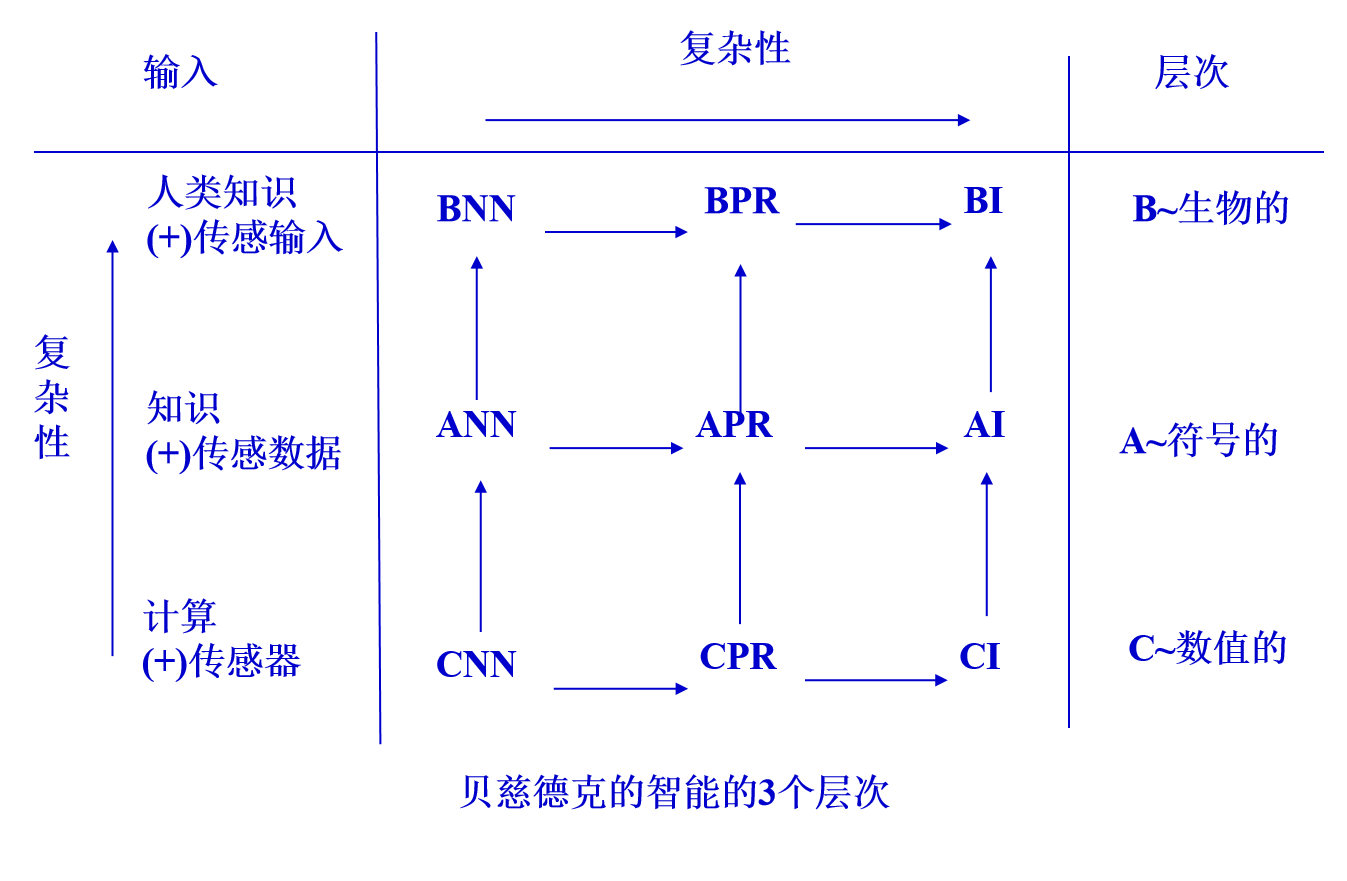
\includegraphics[width=0.6\textwidth]{AI32C42019112601.PNG}
\caption{贝慈德克的智能的3个层次}
\label{AI32fig26000001}
\end{figure}
%%%%%%%%%%%%%%%%%%%%%%%%%%%%%%%%%%%%%%%%%%

第二种观点是大多数学者所持有的观点, 其代表人物是艾伯哈特(R. C. Eberhart). 他们认为: 虽然人工智能与计算智能之间有重合, 但计算智能是一个全新的学科领域, 无论是生物智能还是机器智能, 计算智能都是其最核心的部分, 而人工智能则是外层.
事实上, CI和传统的AI只是智能的两个不同层次, 各自都有自身的优势和局限性, 相互之间只应该互补, 而不能取代.
大量实践证明, 只有把AI和CI很好地结合起来, 才能更好地模拟人类智能, 才是智能科学技术发展的正确方向.
%%%%%%%%%%%%%%%%%%%%%%%%%%%%%%%%%%%%%%
\subsection{计算智能的产生与发展}
1992年, 贝慈德克在《Approximate Reasoning》学报上首次 提出了“计算智能”的概念.

%The International Journal of Approximate Reasoning is intended to serve as a forum for the treatment of imprecision and uncertainty in Artificial and Computational Intelligence, covering both the foundations of uncertainty theories, and the design of intelligent systems for scientific and engineering applications. It publishes high-quality research papers describing theoretical developments or innovative applications, as well as review articles on topics of general interest.
%
%Relevant topics include, but are not limited to, probabilistic reasoning and Bayesian networks, imprecise probabilities, random sets, belief functions (Dempster-Shafer theory), possibility theory, fuzzy sets, rough sets, decision theory, non-additive measures and integrals, qualitative reasoning about uncertainty, comparative probability orderings, game-theoretic probability, default reasoning, nonstandard logics, argumentation systems, inconsistency tolerant reasoning, elicitation techniques, philosophical foundations and psychological models of uncertain reasoning.
%
%Domains of application for uncertain reasoning systems include risk analysis and assessment, information retrieval and database design, information fusion, machine learning, data and web mining, computer vision, image and signal processing, intelligent data analysis, statistics, multi-agent systems, etc. \index{IJAR}
1994年6月底到7月初, IEEE在美国佛罗里达州的奥兰多市召开了首届国际计算智能大会(简称WCCI'94). 会议第一次将神经网络、进化计算和模糊系统这三个领域合并在一起, 形成了“计算智能”这个统一的学科范畴.

在此之后, WCCI大会就成了IEEE的一个系列性学术会议, 每4年举办一次. 1998年5月, 在美国阿拉斯加州的安克雷奇市又召开了第2届计算智能国际会议WCCI’98.
2002年5月, I在美国州夏威夷州首府火奴鲁鲁市又召开了第3届计算智能国际会议WCCI'02.
此外, IEEE还出版了一些与计算智能有关的刊物.
目前, 计算智能的发展得到了国内外众多的学术组织和研究机构的高度重视, 并已成为智能科学技术一个重要的研究领域.

2020年的计算智能会议WCCI2020在英国的格拉斯哥19-24th July. 会议包含三个分会, 2020神经网络国际联合会议 (IJCNN2020), 2020 IEEE模糊系统国际大会 (FUZZ-IEEE 2020)和 2020 IEEE 进化计算代表大会 (IEEE CEC2020).
%%%%%%%%%%%%%%%%%%%%%%%%%%%%%%%%%%%%%%
\section{神经计算}
神经计算也叫神经网络, 是计算智能的重要基础和核心, 也是计算智能乃至智能科学技术的一个重要研究领域.

神经网络是受生物神经元启发构建的计算系统. 神经网络由许多独立的单元组成, 每个单元接收来自上一层单元的输入, 并将输出发送到下个单元(「单元」不一定是单独的物理存在;它们可以被认为是计算机程序的不同组成部分). 单元的输出通常通过取输入的加权和并通过某种简单的非线性转型, 神经网络的关键特性是基于经验修改与单元之间的链接比较相关权重.

\textcolor[rgb]{0,0,1}{常见误解---StuartRussell}

「神经网络是一种新型计算机」. 在实践中, 几乎所有的神经网络都运行在普通的计算机架构上. 一些公司正在设计专用机器, 它们有时会被称作是「神经计算机」, 可以有效地运行神经网络, 但目前为止, 这类机器无法提供足够的优势, 值得花费大量时间去开发.

「神经网络像大脑一样工作」. 事实上, 生物神经元的工作方式比神经网络复杂得多, 自然界存在很多种不同的神经元, 神经元的连接可以随时间进行改变, 大脑中也存在其他的机制, 可以影响动物的行为.

本节的主要内容包括: 神经计算基础、人工神经网络的互连结构和神经网络的典型模型.
%%%%%%%%%%%%%%%%%%%%%%%%%%%%%%%%%%%%%%
\subsection{神经计算基础}
生物神经系统是人工神经网络的基础. 人工神经网络是对人脑神经系统的简化、抽象和模拟, 具有人脑功能的许多基本特征.
为方便对神经网络的进一步讨论, 下面先介绍生物神经元的结构.
%%%%%%%%%%%%%%%%%%%%%%%%%%%%%%%%%%%%%%
\subsubsection{生物神经元的结构}
神经元由细胞体(Soma)、轴突(Axon)和树突(Dendrite)三个主要部分组成:
%%%%%%%%%%%%%%%%%%%%%%%%%%%%%%%%%%%%%%%%%%
\begin{figure}[H]
\centering
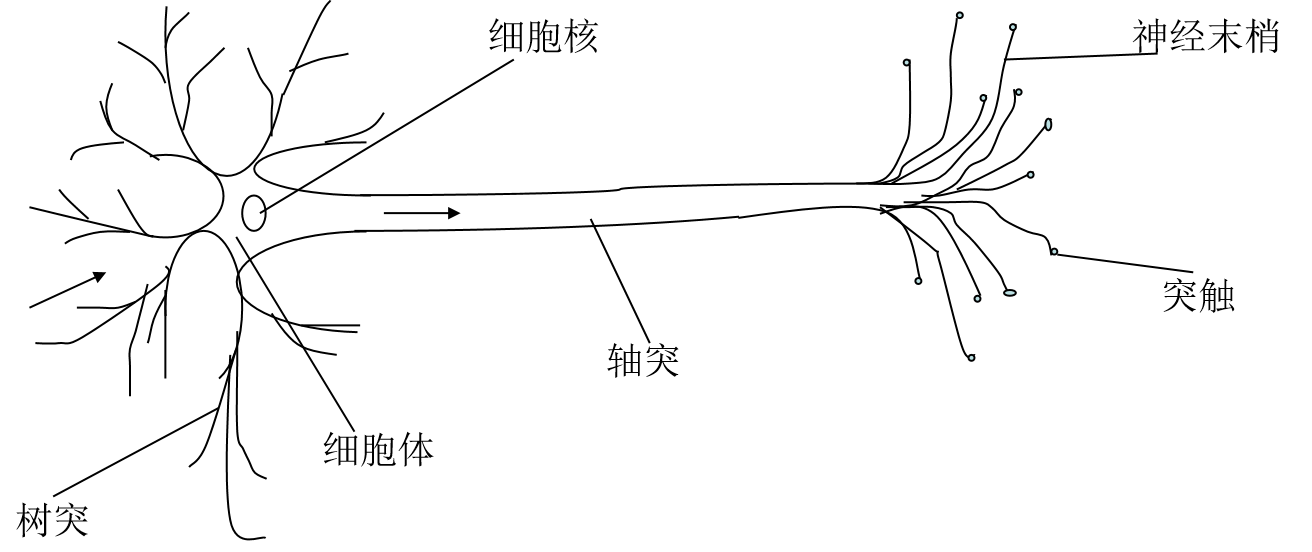
\includegraphics[width=0.76\textwidth]{AI32C42019112602.PNG}
\caption{生物神经元结构}
\label{AI32fig2602}
\end{figure}
%%%%%%%%%%%%%%%%%%%%%%%%%%%%%%%%%%%%%%%%%%
细胞体由细胞核、细胞质和细胞膜等组成, 其直径大约为0.5-100$\si{\mu m}$大小不等. 细胞体是神经元的主体, 用于处理由树突接受的其它神经元传来的信号,其内部是细胞核, 外部是细胞膜, 细胞膜的外面是许多向外延伸出的纤维.

轴突是由细胞体向外延伸出的所有纤维中最长的一条分枝, 用来向外传递神经元产生的输出电信号.
\begin{itemize}
\item 每个神经元都有一条轴突, 其最大长度可达1\si{m}\,以上. 在轴突的末端形成了许多很细的分枝, 这些分支叫\textbf{神经末梢}.
\item 每一条神经末梢可以与其它神经元形成功能性接触, 该接触部位称为突触. 所谓功能性接触, 是指非永久性的接触, 这正是神经元之间传递信息的奥秘之处.
\item 树突是指由细胞体向外延伸的除轴突以外的其它所有分支. 树突的长度一般较短, 但数量很多, 它是神经元的输入端, 用于接受从其它神经元的突触传来的信号.
\end{itemize}
%%%%%%%%%%%%%%%%%%%%%%%%%%%%%%%%%%%%%%
\paragraph{生物神经元的功能}
根据神经生理学的研究, 生物神经元的2个主要功能是: 神经元的兴奋与抑制, 神经元内神经冲动的传导.
\begin{itemize}
\item \ding{172} 神经元的抑制与兴奋

\textbf{抑制状态}是指神经元在没有产生冲动时的工作状态. \textbf{兴奋状态}是指神经元产生冲动时的工作状态.

通常情况下, 神经元膜电位约为-70 毫伏, 膜内为负, 膜外为正, 处于抑制状态. 当神经元受到外部刺激时, 其膜电位随之发生变化, 即膜内电位上升、膜外电位下降, 当膜内外的电位差大于阈值电位(约+40毫伏)时, 神经元产生冲动而进入兴奋状态.

\begin{remark}
  神经元每次冲动的持续时间大约1毫秒左右, 在此期间即使刺激强度再增加也不会引起冲动强度的增加. 神经元每次冲动结束后, 都会重新回到抑制状态. 如果神经元受到的刺激作用不能使细胞膜内外的电位差大于阈值电位, 则神经元不会产生冲动, 将仍处于抑制状态.
\end{remark}

\item \ding{173} 神经元内神经冲动的传导

神经冲动在神经元内的传导是一种电传导过程, 神经冲动沿神经纤维传导的速度却在3.2-320\si{km/s}之间, 且其传导速度与纤维的粗细、髓鞘的有无有一定关系. 一般来说, 有髓鞘的纤维的传导速度较快, 而无髓鞘的纤维的传导速度较慢.
\end{itemize}
%%%%%%%%%%%%%%%%%%%%%%%%%%%%%%%%%%%%%%
\paragraph{人脑神经系统的联结机制}

\quad \ding{172} 人脑神经系统的联结规模

人类大脑中由860-1012亿个神经元所组成, 其中每个神经元大约有$3\times 10^4$个突触. 小脑中的每个神经元大约有$10^5$个突触, 并且每个突触都可以与别的神经元的一个树突相连. 人脑神经系统就是由这些巨量的生物神经元经广泛并行互连所形成的一个高度并行性、非常复杂的神经网络系统.

\quad \ding{173} 人脑神经系统的分布功能

人脑神经系的记忆和处理功能是有机的结合在一起的, 每个神经元既具有存储功能, 同时又具有处理能力. 从结构上看, 人脑神经系统又是一种分布式系统统. 人们通过对脑损坏病人所做的神经生理学研究, 没有发现大脑中的哪一部分可以决定其余所有各部分的活动, 也没有发现在大脑中存在有用于驱动和管理整个智能处理过程的任何中央控制部分. 即, 人类大脑的各个部分是协同工作、相互影响的. 在大脑中, 不仅知识的存储是分散的, 而且其控制和决策也是分散的.
%%%%%%%%%%%%%%%%%%%%%%%%%%%%%%%%%%%%%%
\subsection{人工神经网络的互连结构}
 人工神经网络是由大量的人工神经元经广泛互联所形成的一种人工网络系统, 用以模拟人类神经系统的结构和功能.
%%%%%%%%%%%%%%%%%%%%%%%%%%%%%%%%%%%%%%
\paragraph{人工神经元的结构}
%%%%%%%%%%%%%%%%%%%%%%%%%%%%%%%%%%%%%%
\paragraph{生物神经元的结构}
人工神经元是对生物神经元的抽象与模拟, 图\ref{AI32fig2603}是一个MP神经元模型, 它由细胞体(Soma)、轴突(Axon)和树突(Dendrite)三个主要部分组成,
%%%%%%%%%%%%%%%%%%%%%%%%%%%%%%%%%%%%%%%%%%
%\begin{figure}[H]
%\centering
%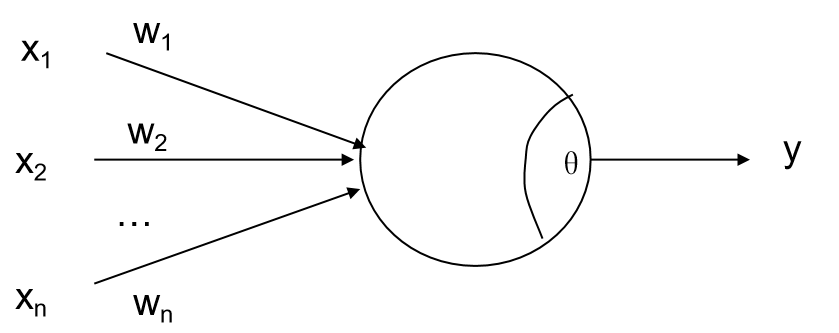
\includegraphics[width=0.6\textwidth]{AI32C42019112603.PNG}
%\caption{MP神经元模型}
%\label{AI32fig2603}
%\end{figure}
%%%%%%%%%%%%%%%%%%%%%%%%%%%%%%%%%%%%%%
\begin{figure}[H]
\begin{center}
\begin{tikzpicture}[line cap=round,line join=round,>=triangle 45,x=1.0cm,y=1.0cm]
\draw(-3,2) circle (1.0cm) node[left, xshift=0.9cm] {\footnotesize $\theta$};
\draw[thick,->](-2,2)--(-0.5,2)node[right, xshift=0.4cm] {\footnotesize $y$};

\draw[thick,->](-6,3)node[left, xshift=-0.2cm] {\footnotesize $x_1$}--(-4,2.07)node[above, xshift=-1.4cm,yshift=1.04cm] {\footnotesize $W_1$};
\draw[thick,->](-6,1.98)node[left, xshift=-0.2cm] {\footnotesize $x_2$}--(-4,1.98)node[above, xshift=-1.4cm] {\footnotesize $W_2$};
\node[above, xshift=0.4cm](cdot) at (-6,1) {\footnotesize $\cdots$};
\draw[thick,->](-6,0.5)node[left, xshift=-0.2cm] {\footnotesize $x_n$}--(-4,1.92)node[above, xshift=-1.4cm,yshift=-1.55cm] {\footnotesize $W_n$};
\end{tikzpicture}
\caption{MP神经元模型}
\label{AI32fig2603}
\end{center}
\end{figure}
%%%%%%%%%%%%%%%%%%%%%%%%%%%%%%%%%%%%%%%%%%%
%%%%%%%%%%%%%%%%%%%%%%%%%%%%%%%%%%%%%%%%%%
%%%%%%%%%%%%%%%%%%%%%%%%%%%%%%%%%%%%%%
\paragraph{常用的人工神经元模型}
根据功能函数的不同, 可得到不同的神经元模型. 常用模型包括:
\begin{itemize}
\item 阈值型(Threshold): 这种模型的神经元没有内部状态, 作用函数$f$是一个阶跃函数, 他表示激活值$\sigma$和输出之间的关系.
\item 分段线性强饱和型(Linear Saturation): 这种模型又称为\textbf{伪线性}, 其输入/输出之间在一定范围内满足线性关系, 一直延续到输出为最大值1为止. 但当达到最大值后, 输出就不再增.
\item S型(Sigmoid)

是一种连续的神经元模型, 其输入输出特性常用指数、对数或双曲正切等S型函数表示. 它反映的是神经元的饱和特性.

\item 子阈累积型(Subthreshold Summation)

是一个非线性函数, 当产生的激活值超过$T$值时, 该神经元被激活产生个反响. 在线性范围内, 系统的反响是线性的.

人工神经网络的互连结构(或称拓扑结构)是指单个神经元之间的连接模式, 它是构造神经网络的基础, 也是神经网络诱发偏差的主要来源. 从互连结构的角度:

仅含输入层和输出层, 且只有输出层的神经元是可计算节点. 除拥有输入、输出层外, 还至少含有一个、或更多个隐含层的前向网络.
\begin{align}
 {y}_{{j}}={f}\left(\sum_{{i}=1}^{{n}} w_{{ij}} {x}_{{i}}-\theta_{{j}}\right), {j}=1,2, \ldots, {m}
\end{align}
\end{itemize}
%%%%%%%%%%%%%%%%%%%%%%%%%%%%%%%%%%%%%%%%%%
%\begin{figure}[H]
%\centering
%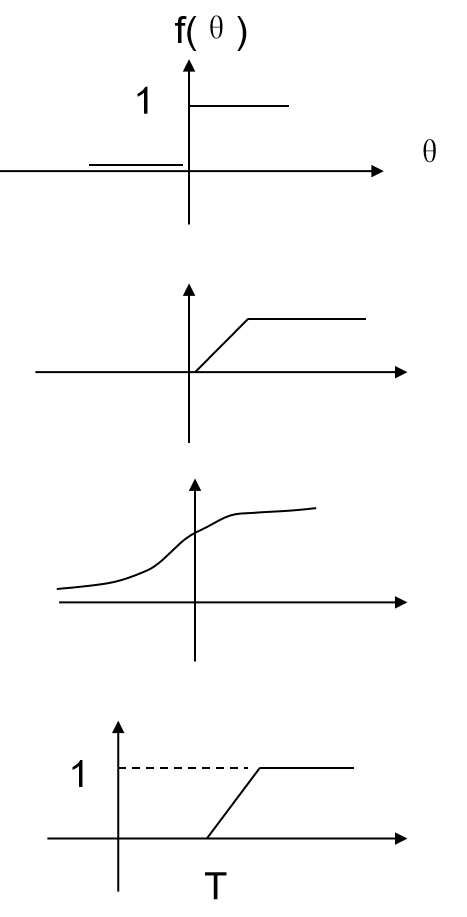
\includegraphics[width=0.5\textwidth]{AI32C42019112604.PNG}
%\caption{MP神经元模型}
%\label{AI32fig2604}
%\end{figure}
%%%%%%%%%%%%%%%%%%%%%%%%%%%%%%%%%%%%%%
\begin{figure}[H]
\begin{center}
\begin{tikzpicture}[line cap=round,line join=round,>=triangle 45,x=1.0cm,y=1.0cm]
\draw[->,color=black] (-5.5,0) -- (-0.2,0);
\draw[->,color=black] (-3.5,-1.05) -- (-3.5,4.03);
\foreach \y in {-1,1,2,3}
\draw[shift={(-3.5,\y)},color=black] (2pt,0pt) -- (-2pt,0pt) ;
% x label and y label O
\node[below,xshift=-0.38cm](origin0) at (-3.5,0) {$O$};
\node[below](axisx) at (-0.3,0) {$x$};
\node[below](axistick11) at (-3.25,2) {$1$};
%fun 1
\draw[thick, -](-5.5,0.0) -- (-3.5,0.0);
\draw[thick, -](-3.5,2.0) -- (-0.25,2.0);
\node[left,xshift=-0.2cm,yshift=0.2cm](axisy) at (-3.5,3.5) {$f(\theta)$};
%% circle
%\draw(-3,2) circle (1.0cm);
%\draw(-3,2) circle (0.05cm) node[left, xshift=0.1cm] {\footnotesize $z_0$};
%\draw[->,color=black, dashed](-3,2)--(-3,1);
%\draw[fill=blue!30](-2.8,2.5) circle (0.05cm)coordinate (z) node[left, xshift=0.1cm] {\footnotesize $z$};
%% right part
%% right 1,2
\draw[->,color=black] (0,0) -- (7.4,0);
\draw[->,color=black] (2.5,-1.05) -- (2.5,4.03);
\foreach \y in {-1,1,2,3}
\draw[shift={(2.5,\y)},color=black] (2pt,0pt) -- (-2pt,0pt) ;
% x label and y label O
\node[below,xshift=-0.38cm](origin0) at (2.5,0) {$O$};
\node[below](axistick12) at (2.25,2) {$1$};
%fun 2
\draw[thick, -](0.0,0.0) -- (2.5,0);
\draw[thick, -](2.5,0) -- (4.5,2);
\draw[thick, -](4.5,2)--(7,2);
\node[below](axisx) at (5.3,0) {$x$};
\node[left,xshift=0.4cm,yshift=0.2cm](axisy) at (2.05,3.5) {$f(\theta)$};
%\draw(3.5,2.4) circle (1.2cm);
%\draw[->,color=black, dashed](3.5,2.4) -- ((3.5,1.2);
%\draw(3.5,2.4)circle (0.05cm)node[right, xshift=0.1cm] {\footnotesize $A$};
%\draw[fill=blue!20](3.2,3.0) circle (0.05cm) coordinate (fz0) node[right, xshift=0.1cm] {\footnotesize $f(z)$};
%\draw[->,color=blue, dashed](z) to [in=120,out=45] (fz0);
%% right 2,1
\draw[->,color=black] (-5.5,-6) -- (-0.2,-6);
\draw[->,color=black] (-3.5,-7) -- (-3.5,-2);
\foreach \y in {-7,-6,-5,-4,-3}
\draw[shift={(-3.5,\y)},color=black] (2pt,0pt) -- (-2pt,0pt) ;
% x label and y label O
\node[below,xshift=-0.38cm](origin0) at (-3.5,-6) {$O$};
\node[below](axisx) at (-0.3,-6) {$x$};
\node[below](axistick11) at (-3.25,-4) {$1$};
%fun 3
\draw[thick, -](-5.5,-6.01) -- (-3.5,-6);
\node[left,xshift=-0.2cm,yshift=0.2cm](axisy) at (-3.5,3.5) {$f(\theta)$};
\draw[scale=1,domain=-5.5:-0.5,smooth,variable=\x,blue] plot ({\x},{-6+2/(1+exp(-3*(\x+3)))});
%\draw[scale=1,domain=0:5,smooth,variable=\x,red] plot ({\x},{1/(1+exp(-3*(\x-1.5)))});
%% circle
%\draw(-3,2) circle (1.0cm);
%\draw(-3,2) circle (0.05cm) node[left, xshift=0.1cm] {\footnotesize $z_0$};
%\draw[->,color=black, dashed](-3,2)--(-3,1);
%\draw[fill=blue!30](-2.8,2.5) circle (0.05cm)coordinate (z) node[left, xshift=0.1cm] {\footnotesize $z$};
%% right part
%% right 2,2
\draw[->,color=black] (0,-6) -- (7.4,-6);
\draw[->,color=black] (2.5,-7.05) -- (2.5,-2.03);
\foreach \y in {-7,-6,-5,-4,-3}
\draw[shift={(2.5,\y)},color=black] (2pt,0pt) -- (-2pt,0pt) ;
% x label and y label O
\node[below,xshift=-0.38cm](origin0) at (2.5,-6) {$O$};
\node[below](axistick12) at (2.25,-4) {$1$};
%fun 4
\draw[thick, -](0.0,-6) -- (4.5,-6);
\draw[thick, -](4.5,-6) -- (5.5,-4);
\draw[thick, -](5.5,-4)--(7,-4);
\draw[dashed,thick, -](2.5,-4)--(5.5,-4);
\node[below](axisx) at (5.3,-6) {$x$};
\node[left,xshift=0.4cm,yshift=0.2cm](axisy) at (2.05,-2.5) {$f(\theta)$};
\end{tikzpicture}
\caption{MP神经元模型}
\label{AI32fig2604}
\end{center}
\end{figure}
%%%%%%%%%%%%%%%%%%%%%%%%%%%%%%%%%%%%%%%%%%%
%%%%%%%%%%%%%%%%%%%%%%%%%%%%%%%%%%%%%%%%%%
%\begin{figure}[H]
%\centering
%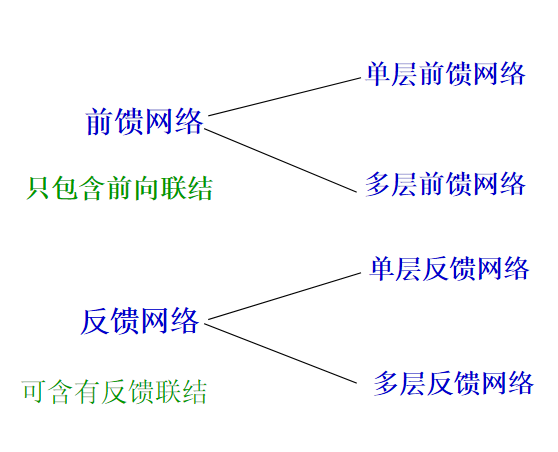
\includegraphics[width=0.6\textwidth]{AI32C42019112605.PNG}
%\caption{MP神经元模型}
%\label{AI32fig2605}
%\end{figure}
%%%%%%%%%%%%%%%%%%%%%%%%%%%%%%%%%%%%%%%%%%
%%%%%%%%%%%%%%%%%%%%%%%%%%%%%%%%%%%%%%
\paragraph{前馈网络}
指不拥有隐含层的反馈网络,包括单层前馈网络和多层前馈网络.

单层前馈网络是指那种只拥有单层计算节点的前向网络. 它仅含有输入层和输出层, 且只有输出层的神经元是可计算节点, 如图\ref{AI32fig1202105}所示.
%%%%%%%%%%%%%%%%%%%%%%%%%%%%%%
\begin{figure}[H]
\begin{center}
\begin{tikzpicture}[font={\sf \small}]
\def \smbwd{2cm}
\def \smbwe{4cm}
\thispagestyle{empty}
%定义流程图的具体形状
\node (qLPV) at (0,0) [draw, process,minimum width=\smbwd, minimum height=0.5cm] {前馈网络};      % 李刚
\node (qLPVtex1) at (0,-0.6) [minimum width=\smbwd, minimum height=0.5cm] {只包含前向链接};      %
\node (UniSampling1)[draw, process,align=center,right=3cm of qLPV,yshift=1cm] {单层前馈网络};%
\node (UniSampling2)[draw, process,align=center,right=3cm of qLPV,yshift=-1cm] {多层前馈网络};%
\draw[->] (qLPV.east)->(UniSampling1)node[left,yshift=0.25cm,rotate=-20,xshift=-1.05cm] {};
\draw[->] (qLPV.east)->(UniSampling2)node[left,yshift=0.25cm,rotate=-20,xshift=-1.05cm] {};
\end{tikzpicture}
\caption{单层前馈网络结构}
\label{AI32fig1202105}
\end{center}
\end{figure}
其中, 输入向量为$X=(x_1,x_2,\cdots,x_n)$; 输出向量为$Y=(y_1,y_2,\cdots,y_m)$; 输入层各个输入到相应神经元的连接权值分别是$w_{ij}, i=1,2,..,n, j=1,2,.., m$.

若假设各神经元的阈值分别是$\theta_j, j=1,2,\cdots,m$, 则各神经元的输出$y_j, j=1,2,\cdots,m$分别为:
\begin{align}
  {y}_{{j}}={f}\left(\sum_{{i}=1}^{{n}} w_{{ij}} {x}_{{i}}-\theta_{{j}}\right), {j}=1,2, \ldots, {m}
\end{align}
其中, 由所有连接权值$w_{ij}$构成的连接权值矩阵$W$为:
\begin{align}
  W=\left(
  \begin{array}{lll}
  {w_{11}} & {w_{12}} & {\cdots w_{1 {m}}} \\ {w_{21}} & {w_{22}} & {\cdots w_{2 {m}}} \\
  {\vdots} & {\vdots} & {\vdots} \\ {w_{{nl}}} & {w_{{n} 2}} & {\cdots w_{{nm}}}.
  \end{array}
  \right)
\end{align}

在实际应用中, 该矩阵是通过大量的训练示例学习而形成的.
%%%%%%%%%%%%%%%%%%%%%%%%%%%%%%%%%%%%%%
\paragraph{多层前馈网络}
多层前馈网络是指那种除拥有输入、输出层外, 还至少含有一个、或更多个隐含层的前馈网络.

隐含层是指由那些既不属于输入层又不属于输出层的神经元所构成的处理层, 也被称为中间层. 隐含层的作用是通过对输入层信号的加权处理, 将其转移成更能被输出层接受的形式.
%%%%%%%%%%%%%%%%%%%%%%%%%%%%%%%%%%%%%%
\paragraph{多层前馈网络结构}

多层前馈网络的输入层的输出向量是第一隐含层的输入信号, 而第一隐含层的输出则是第二隐含层的输入信号, 以此类推, 直到输出层. 多层前馈网络的典型代表是BP网络.
%%%%%%%%%%%%%%%%%%%%%%%%%%%%%%%%%%%%%%
\paragraph{反馈网络}
反馈网络是指允许采用反馈联结方式所形成的神经网络, 图\ref{AI32fig1202205}. 所谓反馈联结方式是指一个神经元的输出可以被反馈至同层或前层的神经元.
%%%%%%%%%%%%%%%%%%%%%%%%%%%%%%
\begin{figure}[H]
\begin{center}
\begin{tikzpicture}[font={\sf \small}]
\def \smbwd{2cm}
\def \smbwe{4cm}
\thispagestyle{empty}
%定义流程图的具体形状
\node (qLPV) at (0,0) [draw, process,minimum width=\smbwd, minimum height=0.5cm] {反馈网络};      % 李刚
\node (qLPVtex1) at (0,-0.6) [minimum width=\smbwd, minimum height=0.5cm] {可含有反馈链接};      %
\node (UniSampling1)[draw, process,align=center,right=3cm of qLPV,yshift=1cm] {单层反馈网络};%
\node (UniSampling2)[draw, process,align=center,right=3cm of qLPV,yshift=-1cm] {多层反馈网络};%
\draw[->] (qLPV.east)->(UniSampling1)node[left,yshift=0.25cm,rotate=-20,xshift=-1.05cm] {};
\draw[->] (qLPV.east)->(UniSampling2)node[left,yshift=0.25cm,rotate=-20,xshift=-1.05cm] {};
\end{tikzpicture}
\caption{单层前馈网络结构}
\label{AI32fig1202205}
\end{center}
\end{figure}
%%%%%%%%%%%%%%%%%%%%%%%%%%%%%%%%%%%%%%
\paragraph{反馈网络和前向网络不同}
前向网络属于非循环连接模式, 它的每个神经元的输入都没有包含该神经元先前的输出, 因此不具有“短期记忆”的性质.

反馈网络则不同, 它的每个神经元的输入都有可能包含有该神经元先前输出的反馈信息, 即一个神经元的输出是由该神经元当前的输入和先前的输出这两者来决定的, 这就有点类似于人类的短期记忆的性质.

反馈网络的典型例子是后面将要介绍的Hopfield网络.
%%%%%%%%%%%%%%%%%%%%%%%%%%%%%%%%%%%%%%
\section{人工神经网络的典型模型}
至于基于神经网络的连接学习机制放到第\ref{AI32PChapter7}章学习部分讨论. 人工神经网络的模型是指对网络结构、联结权值和学习能力的总括. 常用的网络模型已有数十种. 例如:
\begin{itemize}
\item 传统的感知机模型,
\item 具有误差反向传播功能的反向传播网络模型,
\item 采用多变量插值的径向基函数网络模型,
\item 建立在统计学习理论基础上的支撑向量机网络模型,
\item 采用反馈联接方式的反馈网络模型,
\item 基于模拟退火算法的随机网络模型.
\end{itemize}
%%%%%%%%%%%%%%%%%%%%%%%%%%%%%%%%%%%%%%
\subsection{感知机(Perceptron)模型}
感知器是美国学者罗森勃拉特(Rosenblatt)于1957年为研究大脑的存储、学习和认知过程而提出的一类具有自学习能力的神经网络模型, 其拓扑结构是一种分层前向网络.
%%%%%%%%%%%%%%%%%%%%%%%%%%%%%%%%%%%%%%
\paragraph{单层感知器}
单层感知器是一种只具有单层可调节连接权值神经元的前向网络, 这些神经元构成了单层感知器的输出层, 是感知器的可计算节点.

在单层感知器中, 每个可计算节点都是一个线性阈值神经元. 当输入信息的加权和大于或等于阈值时, 输出为1, 否则输出为0或$-1$.

单层感知器的输出层的每个神经元都只有一个输出, 且该输出仅与本神经元的输入及联接权值有关, 而与其他神经元无关.

若假设各神经元的阈值分别是$\theta_j, j=1,2,\cdots,m$, 则各神经元的输出$y_j, j=1,2,\cdots,m$分别为
\begin{align}
  {y}_{{j}}={f}\left(\sum_{{i}=1}^{{n}} w_{{ij}} {x}_{{i}}-\theta_{{j}}\right), {j}=1,2, \ldots, {m}
\end{align}
其中, 由所有连接权值$w_{ji}$构成的连接权值矩阵$W$为
\begin{align}
W=\left(
\begin{array}{llll}
{w_{11}} & {w_{12}} & {\cdots w_{1 {m}}} \\
{w_{21}} & {w_{22}} & {\cdots w_{2 {m}}} \\
{\vdots} & {\vdots} & {} \\
{w_{{n} 1}} & {w_{{n} 2}} & {\cdots} & {w_{{nm}}}.
\end{array}
\right)
\end{align}
在实际应用中, 该矩阵是通过大量的训练示例学习而形成的.

输入向量为$X=(x_1,x_2,\cdots,x_n)$; 输出向量为$Y=(y_1,y_2,\cdots,y_m)$;

输入层各个输入到相应神经元的连接权值分别是$w_{ij},i=1,2,\cdots,n, j=1,2,\cdots, m$.

使用感知器的主要目的是为了对外部输入进行分类. 罗森勃拉特已经证明, 如果外部输入是线性可分的(指存在一个超平面可以将它们分开), 则单层感知器一定能够把它划分为两类. 其判别超平面由如下判别式确定:
\begin{align}
  \sum_{i=1}^{n} w_{i j} x_{i}-\theta_{j}=0 \quad j=1,2, \ldots, m.
\end{align}

下面讨论用单个感知器实现逻辑运算的问题. 事实上, 单层感知器可以很好地实现“与”、“或”、“非”运算, 但却不能解决“异或”问题.
%%%%%%%%%%%%%%%%%%%%%%%%%%%%%%%%%%%%%%%
\begin{example}
  “与”运算($x_1\wedge x_2$)
\end{example}
%%%%%%%%%%%%%%%%%%%%%%%%%%%%%%%%%%%%%%%%%%%
%\begin{figure}[H]
%\centering
%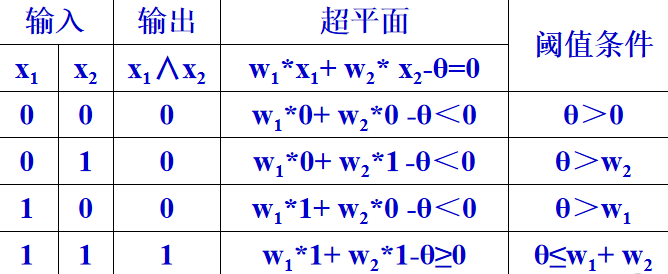
\includegraphics[width=0.6\textwidth]{AI32C42019112606.PNG}
%\caption{}
%\label{AI32fig2606}
%\end{figure}
%%%%%%%%%%%%%%%%%%%%%%%%%%%%%%%%%%%%%%%%%%%
%%%%%%%%%%%%%%%%%%%%%%%%%%%%%%%%%%%%%%%%%%%
%\begin{figure}[H]
%\centering
%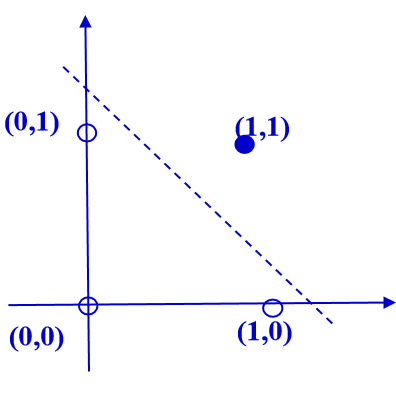
\includegraphics[width=0.6\textwidth]{AI32C42019112607.PNG}
%\caption{}
%\label{AI32fig201912012607}
%\end{figure}
%%%%%%%%%%%%%%%%%%%%%%%%%%%%%%%%%%%%%%%%%%
\begin{figure}[H]
\begin{center}
\begin{tikzpicture}[line cap=round,line join=round,>=triangle 45,x=1.0cm,y=1.0cm]
\draw[->,color=black] (-4.1,0) -- (4.1,0);
\foreach \x in {-4,-3,-2,-1,0,1,2,3}
\draw[shift={(\x,0)},color=black] (0pt,2pt) -- (0pt,-2pt);
%\draw[shift={(\x,0)},color=black] (0pt,2pt) -- (0pt,-2pt) node[below] {\footnotesize $\x$};
\draw[->,color=black] (-2,-2.25) -- (-2,5.03);
\foreach \y in {-2,-1,1,2,3}
\draw[shift={(-2,\y)},color=black] (2pt,0pt) -- (-2pt,0pt);
%\draw[shift={(0,\y)},color=black] (2pt,0pt) -- (-2pt,0pt) node[left] {\footnotesize $\y$};
% x label and y label O
\node[below,xshift=-0.3cm](origin0) at (-2,0) {$O$};
\node[below](axisx) at (3.5,0) {$x$};
\node[left,xshift=-0.2cm](axisy) at (-2,3.5) {$y$};

\draw[fill=blue](1,0) circle (0.1cm)node[below] at (1,0) {$(1,0)$};
\draw[fill=blue](-2,0) circle (0.1cm);
\draw[fill=blue](-2,3) circle (0.1cm) node[below] at (-2,3) {$(0,1)$};
\draw[fill=red](1,3) circle (0.1cm) node[below] at (1,3) {$(1,1)$};
\draw[thick,color=black] (2.85,-1.2) -- (-3,4.6);
% vector
%\draw[->,color=black] (0,0)coordinate (B) -- (3,1.5)coordinate (C)node[right] {\footnotesize $z_1$};
%%\coordinate (A) at (3, 0);
%%% \bar z_1
%\draw[->,color=black] (B) -- (3,-1.5)coordinate (C2)node[right] {\footnotesize $\bar z_1$};
\end{tikzpicture}
\caption{分类曲面}\label{AI32fig201912012607}
\end{center}
\end{figure}
%%%%%%%%%%%%%%%%%%%%%%%%%%%%%%%
\begin{table}[H]
\caption{与运算}
\begin{center}
\begin{tabular} {lccccccccc}
  \hline
输入&输入	&输出&超平面&	阈值条件\\
\hline
$x_1$&$x_2$&$x_1\wedge x_2$	&$w_1\times x_1+ w_2 x_2-\theta=0$  &\\
0&	0&	0&$w_1\times 0+ w_2\times\times 0-\theta \geq 0$ 	&$\theta> 0$\\
0&	1&0	&$w_1\times0 + w_2\times\times 1-\theta \geq 0$ 	&$\theta>w_2$\\
1&	0&	0&$w_1\times1+ w_2\times\times 0 -\theta <0$ 	    &$\theta >w_1$\\
1&	1&	1&$w_1\times0 + w_2\times\times 1-\theta \geq 0$ 	&$\theta\leq w_1+w_2$\\
\hline
\end{tabular}
\end{center}
\label{AI_table2019112900011}
\end{table}

可以证明此表有解, 例如取$w_1=1$, $w_2=1$, $\theta=1.5$, 其分类结果如图\ref{AI32fig201912012607}所示,
其中, 输出为1的用实心圆, 输出为0的用空心圆. 后面约定相同.
%%%%%%%%%%%%%%%%%%%%%%%%%%%%%%%%%%%%
\begin{example}
  “非”运算($\neg x_1$).
\end{example}

表\ref{AI_table2019112902}有解, 例如取$w_1=-1$, $\theta=-0.5$, 其分类结果如右图所示.
%%%%%%%%%%%%%%%%%%%%%%%%%%%%%%%
\begin{table}[H]
\caption{非运算}
\begin{center}
\begin{tabular} {lccccccccc}
  \hline
输入&	输出&	超平面&	阈值条件\\
\hline
$x_1$&	$\neg x_1$&	$w_1*x_1-\theta=0$  &$\theta =0$\\
0&	1&	$w_1*0 -\theta \geq 0$ 	&$\theta\leq 0$\\
1&	0&	$w_1*1 -\theta <0$ 	    &$\theta >w_1$\\
\hline
\end{tabular}
\end{center}
\label{AI_table2019112902}
\end{table}

%%%%%%%%%%%%%%%%%%%%%%%%%%%%%%%%%%%%%%%%%%%%%%%
\begin{example}
  “异或”运算($x_1$ XOR $x_2$).
\end{example}

%%%%%%%%%%%%%%%%%%%%%%%%%%%%%%%
\begin{table}[H]
\caption{异或运算情况表}
\begin{center}
\begin{tabular} {lccccccccc}
  \hline
输入&	输出&	超平面&	阈值条件\\
\hline
$x_1$	&$x_2$	&$x_1$ XOR $x_2$	&$w_1*x_1+ w_2* x_2-\theta=0$&$\theta=0$\\
0	&0	&0	&$w_1*0+ w_2*0 -\theta <0 $&	$\theta >0$\\
0	&1	&1	&$w_1*0+ w_2*1 -\theta \geq 0$ &	$\theta \leq w_2$\\
1	&0	&1	&$w_1*1+ w_2*0 -\theta \geq 0$ &	$\theta \leq w_1$\\
1	&1	&0	&$w_1*1+ w_2*1-\theta <0 $	&   $\theta > w_1+ w_2$\\
\hline
\end{tabular}
\end{center}
\label{AI_table2019112902}
\end{table}
表\ref{Tu9120100511}无解, 即无法找到满足条件的$w_1,w_2$和$\theta$, 如图\ref{Tu9120100511}所示. 因为异或问题是一个非线性可分问题, 需要用多层感知器来解决.
%%%%%%%%%%%%%%%%%%%%%%%%%%%%%%%%%%%%%%%%%%%
%\begin{figure}[H]
%\centering
%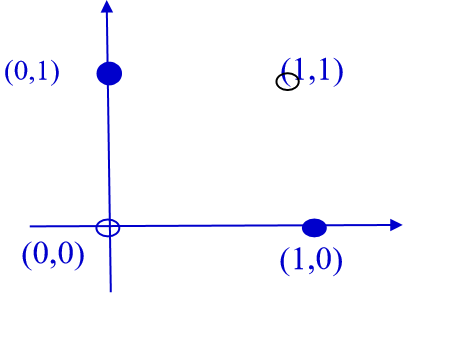
\includegraphics[width=0.56\textwidth]{Tu9120100511.png}
%\caption{}
%\label{Tu9120100511}
%\end{figure}
%%%%%%%%%%%%%%%%%%%%%%%%%%%%%%%%%%%%%%%%%%
\begin{figure}[H]
\begin{center}
\begin{tikzpicture}[line cap=round,line join=round,>=triangle 45,x=1.0cm,y=1.0cm]
\draw[->,color=black] (-4.1,0) -- (4.1,0);
\foreach \x in {-4,-3,-2,-1,0,1,2,3}
\draw[shift={(\x,0)},color=black] (0pt,2pt) -- (0pt,-2pt);
%\draw[shift={(\x,0)},color=black] (0pt,2pt) -- (0pt,-2pt) node[below] {\footnotesize $\x$};
\draw[->,color=black] (-2,-2.25) -- (-2,4.03);
\foreach \y in {-2,-1,1,2,3}
\draw[shift={(-2,\y)},color=black] (2pt,0pt) -- (-2pt,0pt);
%\draw[shift={(0,\y)},color=black] (2pt,0pt) -- (-2pt,0pt) node[left] {\footnotesize $\y$};
% x label and y label O
\node[below,xshift=-0.3cm](origin0) at (-2,0) {$O$};
\node[below](axisx) at (3.5,0) {$x$};
\node[left,xshift=-0.2cm](axisy) at (-2,3.5) {$y$};

\draw[fill=blue](1,0) circle (0.1cm)node[below] at (1,0) {$(1,0)$};
\draw[fill=red](-2,0) circle (0.1cm);
\draw[fill=blue](-2,3) circle (0.1cm) node[below] at (-2,3) {$(0,1)$};
\draw[fill=red](1,3) circle (0.1cm) node[below] at (1,3) {$(1,1)$};
\draw[dashed,color=black] (2.85,-1.2) -- (-3,4.6);
\draw[dashed,color=black] (-1.5,-0.2) -- (2,3.6);
% vector
%\draw[->,color=black] (0,0)coordinate (B) -- (3,1.5)coordinate (C)node[right] {\footnotesize $z_1$};
%%\coordinate (A) at (3, 0);
%%% \bar z_1
%\draw[->,color=black] (B) -- (3,-1.5)coordinate (C2)node[right] {\footnotesize $\bar z_1$};
\end{tikzpicture}
\caption{分类曲面}\label{Tu9120100511}
\end{center}
\end{figure}
%%%%%%%%%%%%%%%%%%%%%%%%%%%%%%%
%%%%%%%%%%%%%%%%%%%%%%%%%%%%%%%%%%%%%%%%%%
%%%%%%%%%%%%%%%%%%%%%%%%%%%%%%%%%%%%%%
\paragraph{多层感知器}
多层感知器是通过在单层感知器的输入、输出层之间加入一层或多层处理单元所构成的. 其拓扑结构与图\ref{Tu9120100509}所示的多层前向网络相似, 差别也在于其计算节点的连接权值是可变的.
%%%%%%%%%%%%%%%%%%%%%%%%%%%%%%%%%%%%%%%%%%%
%\begin{figure}[H]
%\centering
%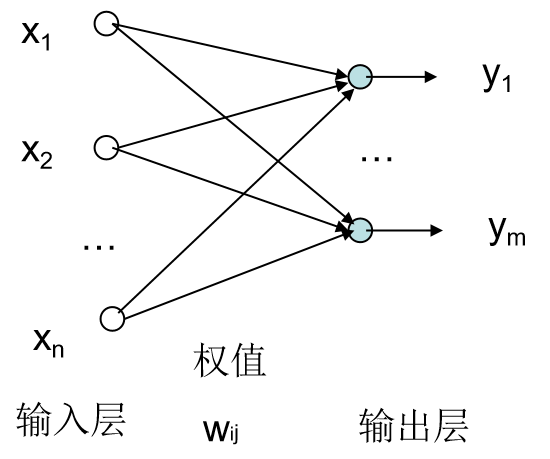
\includegraphics[width=0.56\textwidth]{Tu9120100509.png}
%\caption{}
%\label{Tu9120100509}
%\end{figure}
%%%%%%%%%%%%%%%%%%%%%%%%%%%%%%%%%%%%%%%%%%
\begin{figure}[H]
\begin{center}
\begin{tikzpicture}[line cap=round,line join=round,>=triangle 45,x=1.0cm,y=1.0cm]

%第一层
\draw[fill=blue](0,1) circle (0.15cm)node[xshift=-0.1cm] (x1n) at (0,1) {};
\node[xshift=-0.3cm] (t1n) at (x1n) {$x_1$};
\draw[fill=red](0,2.5) circle (0.15cm)node[xshift=-0.1cm] (x12) at (0,2.5) {};
\node[xshift=-0.3cm] (t12) at (x12) {$x_2$};
\node[yshift=-0.5cm,xshift=0.1cm] (t105) at (x12) {$\vdots$};
\draw[fill=blue](0,4) circle (0.15cm) node[xshift=-0.1cm] (x11)at (0,4) {};
\node[xshift=-0.3cm] (t11) at (x11) {$x_n$};

%第二层
\draw[fill=blue](3,3.5) circle (0.15cm)node[xshift=0.1cm](x2n) at (3,3.5) {};
\node[xshift=1.3cm] (y2n) at (x2n) {$y_n$};
\draw[fill=blue](3,1.5) circle (0.15cm) node[xshift=0.1cm](x21) at (3,1.5) {};
\node[xshift=1.3cm] (y21) at (x21) {$y_1$};
\node[yshift=1cm] (t105) at (x21) {$\vdots$};

\draw[->](x11)--(x2n);
\draw[->](x11)--(x21);

\draw[->](x12)--(x2n);
\draw[->](x12)--(x21);

\draw[->](x1n)--(x2n);
\draw[->](x1n)--(x21);

\draw[->](x21)--(y21);
\draw[->](x2n)--(y2n);

\node[yshift=-0.8cm,xshift=0cm] (text01) at (t1n) {输入层};
\node[yshift=-0.8cm,xshift=1.85cm] (text02) at (t1n) {权重$W_{ij}$};
\node[yshift=-0.8cm,xshift=4cm] (text02) at (t1n) {输出层};
\end{tikzpicture}
\caption{多层感知网络}\label{Tu9120100509}
\end{center}
\end{figure}
%%%%%%%%%%%%%%%%%%%%%%%%%%%%%%%
%%%%%%%%%%%%%%%%%%%%%%%%%%%%%%%%%%%%%%%%%%
多层感知器的输入与输出之间是一种高度非线性的映射关系, 如图\ref{Tu9120100509}所示的多层前向网络, 若采用多层感知器模型, 则该网络就是一个从$n$维欧氏空间到$m$维欧氏空间的非线性映射.
因此, 多层感知器可以实现非线性可分问题的分类.
%%%%%%%%%%%%%%%%%%%%%%%%%%%%%%%%%%%%%%%%
\begin{example}
对“异或”运算, 用图\ref{Tu9120100514}所示的多层感知器即可解决.
%%%%%%%%%%%%%%%%%%%%%%%%%%%%%%%%%%%%%%%%%%%
%\begin{figure}[H]
%\centering
%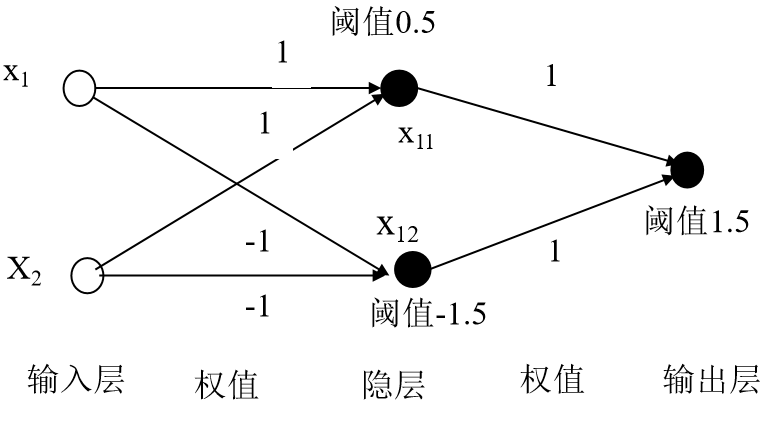
\includegraphics[width=0.6\textwidth]{Tu9120100514.png}
%\caption{}
%\label{Tu9120100514}
%\end{figure}
%%%%%%%%%%%%%%%%%%%%%%%%%%%%%%%%%%%%%%%%%%
\begin{figure}[H]
\begin{center}
\begin{tikzpicture}[line cap=round,line join=round,>=triangle 45,x=1.0cm,y=1.0cm]

%第一层
\draw[fill=blue](0,1) circle (0.15cm)node[xshift=-0.1cm] (x1n) at (0,1) {};
\node[xshift=-0.3cm] (t1n) at (x1n) {$x_2$};
\node[yshift=1.5cm,xshift=0.1cm] (t105) at (x1n) {$\vdots$};
\draw[fill=blue](0,4) circle (0.15cm) node[xshift=-0.1cm] (x11)at (0,4) {};
\node[xshift=-0.3cm] (t11) at (x11) {$x_1$};

%第二层
\draw[fill=blue](3,4) circle (0.15cm)node[xshift=0.1cm](x2n) at (3,4) {};
\node[yshift=-0.4cm] (text12) at (x2n) {$x_{11}$};
\node[yshift=0.6cm,xshift=0cm] (text23) at (x2n) {阈值0.5};
\draw[fill=blue](3,1.) circle (0.15cm) node[xshift=0.1cm](x21) at (3,1.0) {};
\node[yshift=1.5cm] (t105) at (x21) {$\vdots$};
\node[yshift=-0.4cm] (text22) at (x21) {$x_{12}$};
\node[yshift=-0.7cm,xshift=0cm] (text23) at (x21) {阈值-0.5};
%第三层
\draw[fill=blue](5,2.5) circle (0.15cm)node[xshift=0.1cm](x30) at (5,2.5) {};
\node[yshift=-0.6cm,xshift=0.3cm] (text23) at (x30) {阈值1.5};
\node[yshift=0.65cm,xshift=-0.6cm] (text23) at (x30) {1};
\node[yshift=-0.65cm,xshift=-0.6cm] (text23) at (x30) {1};

\draw[->](x11)--(x2n);
\node[yshift=0.4cm,xshift=-1.05cm] (text22) at (x2n) {1};
\node[yshift=-0.9cm,xshift=0cm] (text23) at (text22) {1};
\draw[->](x11)--(x21);
\node[yshift=0.6cm,xshift=-1.05cm] (text22) at (x21) {-1};
\node[yshift=-0.4cm,xshift=0cm] (text23) at (text22) {-1};
\draw[->](x1n)--(x2n);

\draw[->](x1n)--(x21);

\draw[->](x21)--(x30);

\draw[->](x2n)--(x30);

\node[xshift=1.3cm] (x30r) at (x30) {$y$};
\draw[->](x30)--(x30r);

\node[yshift=-1.28cm,xshift=0cm] (text01) at (t1n) {输入层};
\node[yshift=-1.28cm,xshift=1.85cm] (text02) at (t1n) {权值};
\node[yshift=-1.28cm,xshift=3.5cm] (text02) at (t1n) {隐层};
\node[yshift=-1.28cm,xshift=4.25cm] (text02) at (t1n) {权值};
\node[yshift=-1.28cm,xshift=6cm] (text02) at (t1n) {输出层};
\end{tikzpicture}
\caption{异或运算的多层感知网络}\label{Tu9120100514}
\end{center}
\end{figure}
%%%%%%%%%%%%%%%%%%%%%%%%%%%%%%%%%%%%%%%%%%
\end{example}
在图\ref{Tu9120100514}中, 隐层神经元$x_{11}$所确定的直线方程为
\begin{align}
  1 * x_{1}+1 * x_{2}-0.5=0
\end{align}
它可以识别一个半平面. 隐层神经元$x_{12}$所确定的直线方程为
\begin{align}
  1 * x_{1}+1 * x_{2}-1.5=0
\end{align}
它也可以识别一个半平面.

输出层神经元所确定的直线方程为
\begin{align}
  1 * x_{11}+1 * x_{12}-1.5=0
\end{align}
   它相当于对隐层神经元$x_{11}$和$x_{12}$的输出作“逻辑与”运算, 因此可识别由隐层已识别的两个半平面的交集所构成的一个凸多边形, 如图\ref{Tu9120100515}所示.
%%%%%%%%%%%%%%%%%%%%%%%%%%%%%%%%%%%%%%%%%%
%\begin{figure}[H]
%\centering
%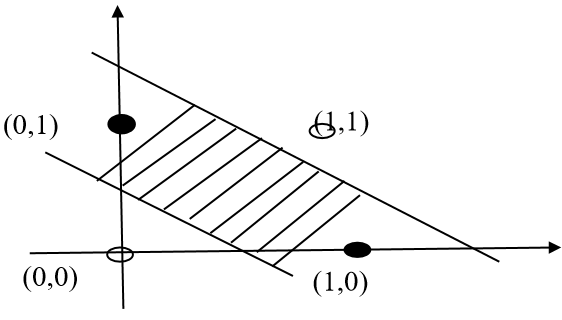
\includegraphics[width=0.6\textwidth]{Tu9120100515.png}
%\caption{}
%\label{Tu9120100515}
%\end{figure}
%%%%%%%%%%%%%%%%%%%%%%%%%%%%%%%%%%%%%%%%%%
\begin{figure}[H]
\begin{center}
\begin{tikzpicture}[line cap=round,line join=round,>=triangle 45,x=1.0cm,y=1.0cm]
\draw[->,color=black] (-4.1,0) -- (4.1,0);
\foreach \x in {-4,-3,-2,-1,0,1,2,3}
\draw[shift={(\x,0)},color=black] (0pt,2pt) -- (0pt,-2pt);
%\draw[shift={(\x,0)},color=black] (0pt,2pt) -- (0pt,-2pt) node[below] {\footnotesize $\x$};
\draw[->,color=black] (-2,-2.25) -- (-2,4.03);
\foreach \y in {-2,-1,1,2,3}
\draw[shift={(-2,\y)},color=black] (2pt,0pt) -- (-2pt,0pt);
%\draw[shift={(0,\y)},color=black] (2pt,0pt) -- (-2pt,0pt) node[left] {\footnotesize $\y$};
% x label and y label O
\node[below,xshift=-0.3cm](origin0) at (-2,0) {$O$};
\node[below](axisx) at (3.5,0) {$x$};
\node[left,xshift=-0.2cm](axisy) at (-2,3.5) {$y$};

\draw[fill=blue](1,0) circle (0.1cm)node[below] at (1,0) {$(1,0)$};
\draw[fill=red](-2,0) circle (0.1cm);
\draw[fill=blue](-2,3) circle (0.1cm) node[below] at (-2,3) {$(0,1)$};
\draw[fill=red](1,3) circle (0.1cm) node[below] at (1,3) {$(1,1)$};
\draw[dashed,color=black] (4.15,-1.2) -- (-3,4.5);
\draw[dashed,color=black] (-4,2) -- (2,-2.7);
%\fill[pattern color=blue,pattern=north west lines] (-2.5,1) -- ++(3.5,2) --  ++(-2.5,-0.8)-- ++(-1.5,-2) -- cycle;%
\fill[pattern color=blue,pattern=north west lines] (-2.7,1.08)--(-1,3)--(1,1.3)--(-0.56,-0.8)-- cycle;
% vector
%\draw[->,color=black] (0,0)coordinate (B) -- (3,1.5)coordinate (C)node[right] {\footnotesize $z_1$};
%%\coordinate (A) at (3, 0);
%%% \bar z_1
%\draw[->,color=black] (B) -- (3,-1.5)coordinate (C2)node[right] {\footnotesize $\bar z_1$};
\end{tikzpicture}
\caption{}\label{Tu9120100515}
\end{center}
\end{figure}
%%%%%%%%%%%%%%%%%%%%%%%%%%%%%%%
%%%%%%%%%%%%%%%%%%%%%%%%%%%%%%%%%%%%%%%%%%
%%%%%%%%%%%%%%%%%%%%%%%%%%%%%%%%%%%%%%
\subsection{反向传播(BP)模型}
误差反向传播(Error Back Propagation)网络通常简称为BP(Back Propagation)网络, 是由美国加州大学的鲁梅尔哈特和麦克莱兰在研究并行分布式信息处理方法, 探索人类认知微结构的过程中, 于1985年提出的一种网络模型.
BP网络的网络拓扑结构是多层前向网络, 如图\ref{Tu9120100516}所示. 在BP网络中, 同层节点之间不存在相互连接, 层与层之间多采用全互连方式, 且各层的连接权值可调. BP网络实现了明斯基的多层网络的设想, 是当今神经网络模型中使用最广泛的一种.
%%%%%%%%%%%%%%%%%%%%%%%%%%%%%%%%%%%%%%%%%%
%\begin{figure}[H]
%\centering
%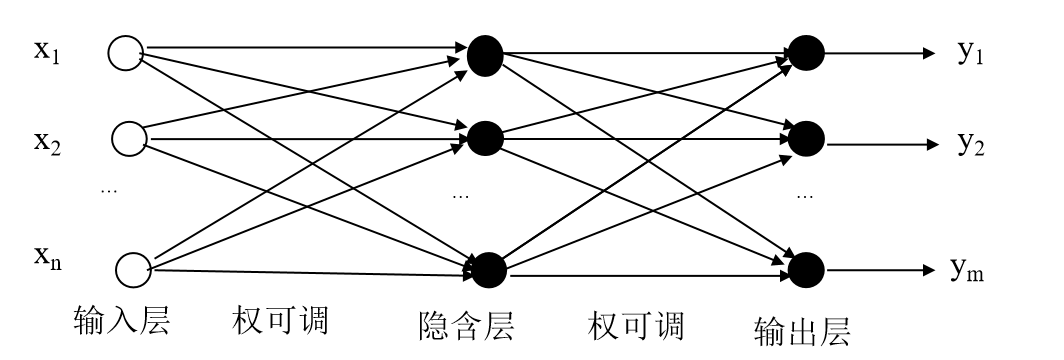
\includegraphics[width=0.56\textwidth]{Tu9120100516.png}
%\caption{多层BP网络的结构}
%\label{Tu9120100516}
%\end{figure}
%%%%%%%%%%%%%%%%%%%%%%%%%%%%%%%%%%%%%%%%%%
\begin{figure}[H]
\begin{center}
\begin{tikzpicture}[line cap=round,line join=round,>=triangle 45,x=1.0cm,y=1.0cm]

%第一层
\draw[](0,1) circle (0.15cm)node[xshift=-0.1cm] (x1n) at (0,1) {};
\node[xshift=-0.3cm] (t1n) at (x1n) {$x_n$};
\draw[](0,2.5) circle (0.15cm)node[xshift=-0.1cm] (x12) at (0,2.5) {};
\node[xshift=-0.3cm] (t12) at (x12) {$x_2$};
\node[yshift=0.95cm,xshift=0.1cm] (t105) at (x1n) {$\vdots$};
\draw[](0,4) circle (0.15cm) node[xshift=-0.1cm] (x11)at (0,4) {};
\node[xshift=-0.3cm] (t11) at (x11) {$x_1$};

%第二层
\draw[fill=blue](3,4) circle (0.15cm)node[xshift=0.1cm](x2n) at (3,4) {};
\node[yshift=-0.4cm] (text12) at (x2n) {$x_{11}$};
\draw[fill=blue](3,2.5) circle (0.15cm)node[xshift=-0.1cm] (x22) at (3,2.5) {};
\node[yshift=-0.3cm] (t22) at (x22) {$x_{12}$};
\node[yshift=-0.5cm,xshift=0.1cm] (t105) at (t22) {$\vdots$};
\draw[fill=blue](3,1.) circle (0.15cm) node[xshift=0.1cm](x21) at (3,1.0) {};
\node[yshift=1.5cm] (t105) at (x21) {$\vdots$};
\node[yshift=-0.4cm] (text22) at (x21) {$x_{1n}$};
%第三层
\draw[fill=blue](6,4) circle (0.15cm)node[xshift=0.1cm](x3n) at (6,4) {};
\draw[fill=blue](6,1) circle (0.15cm)node[xshift=0.1cm](x31) at (6,1) {};
\draw[fill=blue](6,2.5) circle (0.15cm)node[xshift=0.1cm](x32) at (6,2.5) {};
\node[yshift=-0.5cm,xshift=-0.1cm] (t105) at (x32) {$\vdots$};

\draw[->](x11)--(x2n);
\draw[->](x11)--(x21);
\draw[->](x11)--(x22);

\draw[->](x12)--(x2n);
\draw[->](x12)--(x21);
\draw[->](x12)--(x22);

\draw[->](x1n)--(x2n);
\draw[->](x1n)--(x21);
\draw[->](x1n)--(x22);

\draw[->](x1n)--(x2n);
\draw[->](x1n)--(x21);

\draw[->](x21)--(x3n);
\draw[->](x21)--(x32);
\draw[->](x21)--(x31);

\draw[->](x22)--(x3n);
\draw[->](x22)--(x32);
\draw[->](x22)--(x31);

\draw[->](x2n)--(x3n);
\draw[->](x2n)--(x32);
\draw[->](x2n)--(x31);

\node[xshift=1.3cm] (x3nh1) at (x3n) {$y_1$};
\node[xshift=1.3cm] (x32h1) at (x32) {$y_2$};
\node[yshift=-0.5cm,xshift=-0.1cm] (t105) at (x32h1) {$\vdots$};
\node[xshift=1.3cm] (x3nh2) at (x31) {$y_m$};
\draw[->](x31)--(x3nh2);
\draw[->](x32)--(x32h1);
\draw[->](x3n)--(x3nh1);

\node[yshift=-1.28cm,xshift=0cm] (text01) at (t1n) {输入层};
\node[yshift=-1.28cm,xshift=1.85cm] (text02) at (t1n) {权可调};
\node[yshift=-1.28cm,xshift=3.5cm] (text02) at (t1n) {隐层};
\node[yshift=-1.28cm,xshift=5.25cm] (text02) at (t1n) {权可调};
\node[yshift=-1.28cm,xshift=6.6cm] (text02) at (t1n) {输出层};
\end{tikzpicture}
\caption{多层BP网络的结构}\label{Tu9120100516}
\end{center}
\end{figure}
%%%%%%%%%%%%%%%%%%%%%%%%%%%%%%%%%%%%%%%%%%
对BP网络需说明以下两点:
\begin{itemize}
\item 第一, BP网络的每个处理单元均为非线性输入/输出关系, 其作用函数通常采用的是可微的Sigmoid函数, 如:
\begin{align}
  f(x)=\frac{1}{1+e^{-x}}.
\end{align}
\item 第二, BP网络的学习过程是由工作信号的正向传播和误差信号的反向传播组成的. 所谓正向传播, 是指输入模式经隐层到输出层, 最后形成输出模式; 所谓误差反向传播, 是指从输出层开始逐层将误差传到输入层, 并修改各层联接权值, 使误差信号为最小的过程.
\end{itemize}
%%%%%%%%%%%%%%%%%%%%%%%%%%%%%%%%%%%%%%
\subsection{反馈网络(Hopfield)模型}
Hopfield网络是由美国加州工学院物理学家霍普菲尔特1982年提出来的一种单层全互连的对称反馈网络模型. 它可分为离散Hopfield网络和连续Hopfield网络, 限于篇幅, 本书重点讨论离散Hopfield网络.
%%%%%%%%%%%%%%%%%%%%%%%%%%%%%%%%%%%%%%
\paragraph{离散Hopfield网络的结构}
%%%%%%%%%%%%%%%%%%%%%%%%%%%%%%%%%%%%%%%%%%
%\begin{figure}[H]
%\centering
%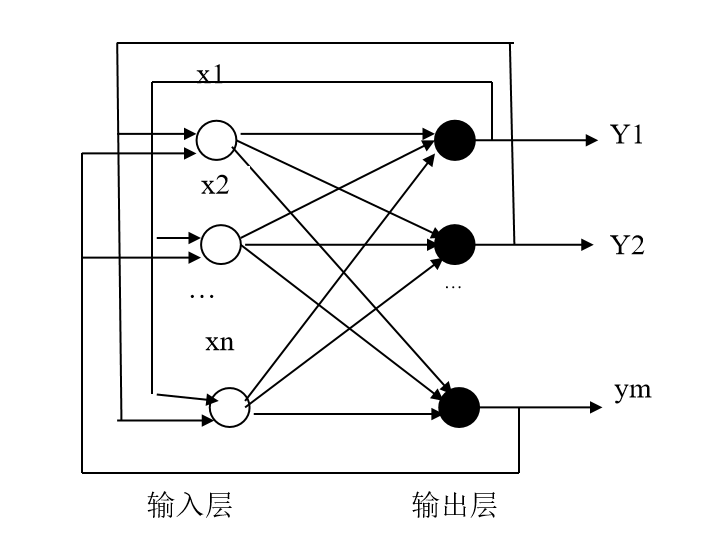
\includegraphics[width=0.6\textwidth]{AI32C42019112608.PNG}
%\caption{离散Hopfield网络}
%\label{AI32fig201912022608}
%\end{figure}
%%%%%%%%%%%%%%%%%%%%%%%%%%%%%%%%%%%%%%%%%%
\begin{figure}[H]
\begin{center}
\begin{tikzpicture}[line cap=round,line join=round,>=triangle 45,x=1.0cm,y=1.0cm]

%第一层
\draw[](0,1) circle (0.15cm)node[xshift=-0.1cm] (x1n) at (0,1) {};
\node[xshift=-0.3cm,yshift=0.3cm] (t1n) at (x1n) {$x_n$};
\draw[](0,2.5) circle (0.15cm)node[xshift=-0.1cm] (x12) at (0,2.5) {};
\node[xshift=-0.3cm,yshift=0.3cm] (t12) at (x12) {$x_2$};
\node[yshift=0.95cm,xshift=0.1cm] (t105) at (x1n) {$\vdots$};
\draw[](0,4) circle (0.15cm) node[xshift=-0.1cm] (x11)at (0,4) {};
\node[xshift=-0.3cm,yshift=0.3cm] (t11) at (x11) {$x_1$};

%第二层
\draw[fill=blue](3,4) circle (0.15cm)node[xshift=0.1cm](x2n) at (3,4) {};
\node[yshift=-0.4cm] (text12) at (x2n) {$x_{11}$};
\draw[fill=blue](3,2.5) circle (0.15cm)node[xshift=-0.1cm] (x22) at (3,2.5) {};
\node[yshift=-0.3cm] (t22) at (x22) {$x_{12}$};
\node[yshift=-0.5cm,xshift=0.1cm] (t105) at (t22) {$\vdots$};
\draw[fill=blue](3,1.) circle (0.15cm) node[xshift=0.1cm](x21) at (3,1.0) {};
\node[yshift=1.5cm] (t105) at (x21) {$\vdots$};
\node[yshift=-0.4cm] (text22) at (x21) {$x_{1n}$};
%第三层
\node[xshift=2.4cm] (text31) at (x21) {$y_{m}$};
\node[xshift=2.4cm] (text32) at (x22) {$y_{2}$};
\node[xshift=2.4cm] (text3n) at (x2n) {$y_{1}$};

% 返回线

\node[xshift=1.4cm,yshift=0.15cm] (text01) at (x21) {};
\node[xshift=1.4cm,yshift=-0.15cm] (text02) at (x22) {};
\node[xshift=1.4cm,yshift=-0.15cm] (text0n) at (x2n) {};

\draw[->](text01)--++(0,-1)--++(-6,0)--++(0,0.9)--++(1.34,0); %y_n
\draw[->](text01)--++(0,-1)--++(-6,0)--++(0,2.3)--++(1.34,0);

\draw[->](text0n)--++(0,1)--++(-6.6,0)--++(0,-2.385)--++(1.95,0); %y_1
\draw[->](text0n)--++(0,1)--++(-6.6,0)--++(0,-3.81)--++(1.95,0); %y_1

\draw[blue,->](text02)--++(0,2)--++(-6,0)--++(0,-0.4)--++(1.55,0); %y_2
\draw[blue,->](text02)--++(0,2)--++(-6,0)--++(0,-3.3)--++(1.55,0); %y_2

\draw[->](x21)--(text31);
\draw[blue,->](x22)--(text32);
\draw[->](x2n)--(text3n);

\draw[->](x11)--(x2n);
\draw[->](x11)--(x21);
\draw[->](x11)--(x22);

\draw[->](x12)--(x2n);
\draw[->](x12)--(x21);
\draw[->](x12)--(x22);

\draw[->](x1n)--(x2n);
\draw[->](x1n)--(x21);
\draw[->](x1n)--(x22);

\draw[->](x1n)--(x2n);
\draw[->](x1n)--(x21);

\node[yshift=-2.28cm,xshift=0cm] (text01) at (t1n) {输入层};
\node[yshift=-2.28cm,xshift=3cm] (text02) at (t1n) {输出层};
\end{tikzpicture}
\caption{离散Hopfield网络}
\label{AI32fig201912022608}
\end{center}
\end{figure}
%%%%%%%%%%%%%%%%%%%%%%%%%%%%%%%%%%%%%%%%%%
离散Hopfield网络是在非线性动力学的基础上由若干基本神经元构成的一种单层全互连网络, 其任意神经元之间均有连接, 并且是一种对称连接结构. 一个典型的离散 Hopfidld网络结构如图\ref{AI32fig201912022608}所示. 离散Hopfield网络模型是一个离散时间系统, 每个神经元只有0和1(或-1和1)两种状态, 任意神经元$i$和$j$之间的连接权值为$w_{ij}$. 由于神经元之间为对称连接, 且神经元自身无连接, 因此有
\begin{align}
  w_{i j}=\left\{
  \begin{array}{ll}
  {w_{j i}}, & i \neq j \\
    {0}, &  i=j
    \end{array}\right.
\end{align}
由该连接权值所构成的连接矩阵是一个零对角的对称矩阵. 在 Hopfidld网络中, 虽然神经元自身无连接, 但由于每个神经元都与其他神经元相连, 即每个神经元的输出都将通过突触连接权值传递给别的神经元, 同时每个神经元又都接受其他神经元传来的信息, 这样对每个神经元来说, 其输出经过其他神经元后又有可能反馈给自己, 因此Hopfidld网络是一种反馈神经网络.
%%%%%%%%%%%%%%%%%%%%%%%%%%%%%%%%%%%%%%
\section{其它神经学习算法}
%%%%%%%%%%%%%%%%%%%%%%%%%%%%%%%%%%%%%%
\subsection{ELM}
Fig.\ref{OPELM20161021fig2} shows the three steps of OP-ELM. The optimally pruned extreme learning machine (OP-ELM) is proposed in (EIML Group. The op-elm toolbox, Available online at /http://www.cis.hut.fi/projects/eiml/research/download ``corrupt" some of the neurons. As described at more length in \cite{Miche2008OP, Miche2008A, Miche2010OP}, it can be illustrated on a toy example as in Fig. 1: the plots give the ELM fit in light blue dots over the training points in black crosses. On the leftmost part of the figure,
the fit by the ELM is good, but when a pure random noise variable is added, on the rightmost figure (the added noise variable is not pictured on the figure), the fit becomes loose and spread.

Indeed, the ELM is not designed to cope with such variables irrelevant to the problem at hand. In this spirit, the \textbf{OP-ELM} proposes a three-steps methodology, shortly described here, to address this issue. The idea is to build a wrapper around the original ELM, with a neuron pruning strategy. For this matter, as can be seen in Fig. 2, the construction of the SLFN by the ELM is retained, and two steps are added afterwards. First comes a ranking of the neurons by a least angle regression (LARS \cite{EfronHastie2004-32498}; in practice the \textbf{MRSR} \index{MRSR}\cite{SimiläTikka2005-32497} implementation of LARS is used for it also applies to multi-output cases), which sorts them by their usefulness regarding the output. And then a leave-one-out criterion is used to determine how many of the-sorted-neurons should be kept for the final OP-ELM model structure.

The \textbf{LARS algorithm} is not detailed here since it is described and discussed at length (or more precisely the idea it implements, Lasso) in Section 3, but it has the property of providing an exact ranking of the hidden-layer neurons in the case of the OP-ELM, since the relation between the neurons and the output is linear (by design of the OP-ELM).

The \textbf{leave-one-out}\index{Leave-one-out(LOO)} (LOO) method is usually a costly approach to optimize a parameter since it requires to train the model on the whole data set but one sample, and evaluate on this sample, repeatedly for all the samples of the data set. In the OP-ELM structure though, the situation is linear (between the hidden layer and the output one), and the LOO error has a closed matrix form, given by \textbf{Allen's prediction sum of squares} (PRESS)\index{PRESS} \cite{MADavid1972} (details of the computation of the PRESS LOO error are given in Section 4). This closed form allows for fast computation of the mean square error and hence of the output weights $\bm b$, making the OP-ELM still computationally efficient and more robust than the original ELM to irrelevant/ correlated variables. Hence, the OP-ELM can be seen as a ``regularized" ELM, by the use of a \textbf{LARS}\index{LARS} approach, which is a $L_1$ penalty on a regression problem, here.

Meanwhile, the decision over the final number of neurons to retain (by a \textbf{LOO criterion}\index{LOO criterion}) has shown potential instabilities (numerically), due to the nature of the matrix operations performed in the PRESS formula (see Section 4 for these calculations). The proposed solution in this paper is to use regularization in the calculations of the PRESS formula. In the following are reviewed the most well-known algorithms used to perform regularization, using a $L_1$ and $L_2$ (and jointly $L_1$ and $L_2$) penalty on the regression problem. The proposed approach in Section 4 combines both $L_1$ and $L_2$ penalties in the OP-ELM, to regularize the network.
\begin{figure}[t]
\begin{center}
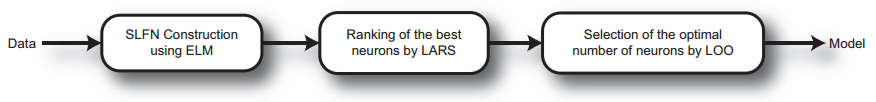
\includegraphics[scale=0.7]{OPELM20161021.PNG}
\end{center}
\caption{Illustration of the three OP-ELM steps: the SLFN is first built using the ELM approach (random initialization of internal weights and biases); then a LARS algorithm is
used to rank the neurons of the hidden layer; finally the selection of the optimal number of neurons for the OP-ELM model is performed using a Leave-One-Out criterion.}
\label{OPELM20161021fig2}
\end{figure}
%%%%%%%%%%%%%%%%%%%%%%%%%%%%%%%%%%%%%%%%%%%
\subsubsection{Tikhonov regularization}\index{Tikhonov Regularization}
Tikhonov regularization, named for Andrey Tikhonov, is the most commonly used method of regularization of ill-posed problems. In statistics, the method is known as \textbf{ridge regression}\index{Ridge Regression}, and with multiple independent discoveries, it is also variously known as the \textbf{Tikhonov–Miller method}\index{Tikhonov–Miller method}, the \textbf{Phillips–Twomey method}\index{Phillips–Twomey method}, the \textbf{Constrained linear inversion method}, and the method of \textbf{linear regularization}\index{Linear regularization}. It is related to the \textbf{Levenberg–Marquardt algorithm} for \textbf{non-linear least-squares}\index{Non-linear least-squares} problems.

Suppose that for a known matrix $\bm A$ and vector $\bm b$, we wish to find a vector $\bm {x}$ such that
\begin{align}
   \bm A\bm {x} =\bm {b}.
\end{align}
The standard approach is ordinary least squares linear regression. However, if no $\bm x$ satisfies the equation or more than one $\displaystyle x$ does—that is the solution is not unique—the problem is said not to be well posed. In such cases, ordinary least squares estimation leads to an overdetermined (over-fitted), or more often an underdetermined (under-fitted) system of equations. Most real-world phenomena have the effect of \textbf{low-pass filters} in the forward direction where $\displaystyle A$ maps $ \bm {x}$ to $ \bm {b}$. Therefore, in solving the inverse-problem, the inverse mapping operates as a high-pass filter that has the undesirable tendency of amplifying noise (eigenvalues / singular values are largest in the reverse mapping where they were smallest in the forward mapping). In addition, ordinary least squares implicitly nullifies every element of the reconstructed version of $\bm {x}$ that is in the null-space of $A$, rather than allowing for a model to be used as a prior for $\bm {x}$. Ordinary least squares seeks to minimize the sum of squared residuals, which can be compactly written as
\begin{align}
   \|\bm A\bm {x} -\bm {b} \|^{2}
\end{align}
where $\left\|\cdot \right\|$ is the Euclidean norm. In order to give preference to a particular solution with desirable properties, a regularization term can be included in this minimization:
\begin{align}
  \|\bm A\bm {x} -\bm {b} \|^{2}+\|\Gamma \bm {x} \|^{2}
\end{align}
for some suitably chosen \textbf{Tikhonov matrix}, $\Gamma$. In many cases, this matrix is chosen as a multiple of the identity matrix $ (\Gamma =\alpha I)$, giving preference to solutions with smaller norms; this is known as $L_2$ regularization \cite{Ng2004-32636}. In other cases, \textbf{lowpass operators}\index{Lowpass Operators} (e.g., a difference operator or a \textbf{weighted Fourier operator}\index{Fourier operator}) may be used to enforce smoothness if the underlying vector is believed to be mostly continuous. This regularization improves the conditioning of the problem, thus enabling a direct numerical solution. An explicit solution, denoted by $\hat {x}$, is given by:
\begin{align}
  {\hat {x}}=(\bm A^{T}\bm A+\Gamma ^{T}\Gamma )^{-1}\bm A^{T}\bm {b}
\end{align}

The effect of regularization may be varied via the scale of matrix $\Gamma$. For $ \Gamma =0$ this reduces to the unregularized least squares solution provided that $(A^TA)^{-1}$ exists.

$L_2$ regularization is used in many contexts aside from linear regression, such as classification with logistic regression or support vector machines \cite{Fan2008LIBLINEAR}, and matrix factorization \cite{Guan2012Online}.

\textbf{Tikhonov regularization} has been invented independently in many different contexts. It became widely known from its application to integral equations from the work of Andrey Tikhonov and David L. Phillips. Some authors use the term \textbf{Tikhonov–Phillips regularization}. The finite-dimensional case was expounded by Arthur E. Hoerl, who took a statistical approach, and by Manus Foster, who interpreted this method as a \textbf{Wiener–Kolmogorov (Kriging) filter}. Following Hoerl, it is known in the statistical literature as \textbf{ridge regression}.

\textbf{Generalized Tikhonov regularization}

For general multivariate normal distributions for $\bm x$ and the data error, one can apply a transformation of the variables to reduce to the case above. Equivalently, one can seek an $\bm x$ to minimize
\begin{align}
  \|\bm A\bm x-\bm b\|_{P}^{2}+\|\bm x-\bm x_{0}\|_{Q}^{2}\,
\end{align}
where we have used $\left\|\bm x\right\|_{\bm Q}^{2}$ to stand for the weighted norm $ \bm x^{T}\bm Q\bm x$ (compare with the Mahalanobis distance). In the Bayesian interpretation $\bm P$ is the inverse covariance matrix of $\bm b, \bm x_0$ is the expected value of $x$, and $\bm Q$ is the inverse covariance matrix of $\bm x$. The Tikhonov matrix is then given as a factorization of the matrix $\displaystyle \bm Q=\Gamma ^{T}\Gamma$ (e.g. the \textbf{Cholesky factorization}), and is considered a \textbf{whitening filter}.

This generalized problem has an optimal solution $x^{*}$ which can be solved explicitly using the formula
\begin{align}
  \bm x^{*}=(\bm A^{T}\bm P\bm A+\bm Q)^{-1}(\bm A^{T}\bm P\bm b+\bm Q\bm x_{0}).\,
\end{align}
or equivalently
\begin{align}
  \bm x^{*}=\bm x_{0}+(\bm A^{T}\bm P\bm A+\bm Q)^{-1}(\bm A^{T}\bm P(\bm b-\bm A \bm x_{0})).\,
\end{align}
%%%%%%%%%%%%%%%%%%%%%%%%%%%%%%%%%%%%%%%%%%%
\subsection{TROP-ELM}\index{TROP-ELM}
\textbf{TROP-ELM}: A double-regularized ELM using LARS and Tikhonov regularization \cite{MichevanHeeswijk2011-30641}, 2011.

Fig. \ref{TROPEMLmodel20161021fig2} shows the proposed regularized OP-ELM (TROP-ELM).
\begin{figure}[H]
\begin{center}
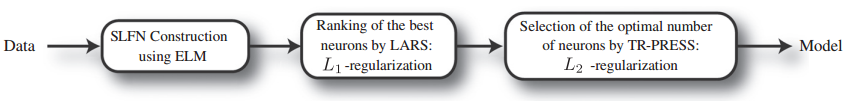
\includegraphics[scale=0.7]{TROPEMLmodel20161021.PNG}
\end{center}
\caption{The proposed regularized OP-ELM (TROP-ELM) as a modification of Fig. \ref{OPELM20161021fig2}.}
\label{TROPEMLmodel20161021fig2}
\end{figure}
%%%%%%%%%%%%%%%%%%%%%%%%%%%%%%%%%%%%
\subsection{Allen's PRESS(prediction sum of squares)}
The original PRESS formula used in the OP-ELM was proposed by Allen in \cite{MADavid1972}. The original PRESS formula can be expressed as
\begin{align}
  \textup{MSE}^{\textup{TR-PRESS}}=\frac 1 n \sum_{i=1}^n \left( \frac{y_i-\bm x_i(\bm X^T \bm X)^{-1}\bm x^T y  }
       {1-\bm x_i(\bm X^T \bm X)^{-1}\bm x_i^T}\right)^2,
\end{align}
which means that each observation is ``predicted" using the other $n-1$ observations and the residuals are finally squared and summed up. Algorithm \ref{AllenPRESS161018Algorithm1} proposes to implement this formula in an efficient way, by matrix computations.

\textbf{Algorithm 1.}
%%%%%%%%%%%%%%%%%%%%%%%%%%%%%%%%%%%%%
%\begin{algorithm}
%\caption{Allen's PRESS algorithm.}
%\label{AllenPRESS161018Algorithm1}
%\begin{algorithmic}[1] %
%\STATE Compute the utility matrix $\bm C= (\bm X^T X)^{-1}$
%\STATE And $\bm P = \bm X\bm C$;
%\STATE Compute the pseudo-inverse $\bm w = \bm C\bm X^T\bm y$;
%\STATE  Compute the denominator of the PRESS $D = \bm 1-\diag(\bm P\bm X^T)$;
%\STATE And finally the PRESS error $e = \frac{y-\bm X \bmw} {\bm D} $;
%\STATE Reduced to a $\textup{MSE}^{\textup{TR-PRESS}}=\frac 1 n \sum_{i=1}^n \epsilon_i^2$
% \end{algorithmic}
%\end{algorithm}
1: Compute the utility matrix $\bm C= (\bm X^T X)^{-1}$

2: And $\bm P = \bm X\bm C$;

3: Compute the pseudo-inverse $\bm w = \bm C\bm X^T\bm y$;

4: Compute the denominator of the PRESS $D = \bm 1-\textup{diag}(\bm P\bm X^T)$;

5: And finally the PRESS error $e = \frac{y-\bm X \bm w} {\bm D} $;

6: Reduced to a $\textup{MSE}^{\textup{TR-PRESS}}=\frac 1 n \sum_{i=1}^n \epsilon_i^2$

The main drawback of this approach lies in the use of a pseudo-inverse in the calculation (in the \textbf{Moore–Penrose sense}), which can lead to numerical instabilities if the data set $\bm X$ is not full rank. This is unfortunately very often the case, with real world data sets. The following approach proposes two improvements on the computation of the original \textbf{PRESS}: regularization and fast matrix calculations.
%%%%%%%%%%%%%%%%%%%%%%%%%%%%%%%%%%%%%%%%%%%%%%%%%%%%%%%
\subsubsection{Tikhonov-regularized PRESS (TR-PRESS)}
In \cite{Golub1979Generalized}, Golub et al. note that the singular value decomposition (SVD) approach to compute the PRESS statistic is preferable to the traditional pseudo-inverse mentioned above, for numerical reasons. In this very same paper is proposed a generalization of Allen's PRESS, as the \textbf{generalized cross-validation} (GCV) method, which is technically superior to the original \textbf{PRESS}, for it can handle cases were the data is extremely badly defined—for example if all $X$ entries are 0 except the diagonal ones.

In practice, from our experiments, while the GCV is supposably superior, it leads to identical solutions with an increased computational time, compared to the original \textbf{PRESS} and the Tikhonov regularized version of PRESS presented below. Algorithm 1 gives the computational steps used, in matrix form, to determine the $\textup{MSE}^{\textup{TR-PRESS}}$ from
\begin{align}
  \textup{MSE}^{\textup{TR-PRESS}}=\frac 1 n \sum_{i=1}^n \left( \frac{y_i-\bm x_i(\bm X^T \bm X+\lambda \bm I)^{-1}\bm x^T y  }
       {1-\bm x_i(\bm X^T \bm X+\lambda \bm I)^{-1}\bm x_i^T}\right)^2
\end{align}
which is the regularized version of Eq. (18). The notation $A\circ B$ denotes element-wise product between matrices $\bm A$ and $\bm B$ (Schur product). It is used in step 4 of Algorithm 2 for it is faster than standard matrix product.
%%%%%%%%%%%%%%%%%%%%%%%%%%%%%%%%%%%%%%
%\begin{algorithm}
%\caption{Tikhonov-regularized PRESS.}
%\label{Tikhonov-regularizedPRESS161018Algorithm2}
%\begin{algorithmic}[1] %
%\STATE Decompose $\bm X$ by SVD: $\bm X = \bm U\bm S\bm V^T$;
%\STATE Compute the products (used later): $A = \bm X\bm V$ and $B = \bm U^T\bm y$;
%\STATE repeat
%\STATE Using the SVD of $\bm X$, compute the $\bm C$ matrix by:
%\STATE Compute the $\bm P$ matrix by: $\bm P = \bm C\bm B$;
%\STATE Compute $\bm D$ by: $\bm D = \bm 1-\diag(\bm C\bm U^T)$;
%\STATE Evaluate $e = \frac{y-\bm P} {\bm D}$ and the actual  MSE by $\textup{MSE}^{\textup{TR-PRESS}}=\frac 1 n \sum_{i=1}^n \epsilon_i^2$.
%\STATE \textbf{until} convergence on $\lambda$ is achieved
%\STATE Keep the best $\textup{MSE}^{\textup{TR-PRESS}}$ and the $\lambda$ value associated.
% \end{algorithmic}
%\end{algorithm}

Decompose $\bm X$ by SVD: $\bm X = \bm U\bm S\bm V^T$;

Compute the products (used later): $A = \bm X\bm V$ and $B = \bm U^T\bm y$;

repeat

Using the SVD of $\bm X$, compute the $\bm C$ matrix by:

Compute the $\bm P$ matrix by: $\bm P = \bm C\bm B$;

Compute $\bm D$ by: $\bm D = \bm 1-\textup{diag}(\bm C\bm U^T)$;

Evaluate $e = \frac{y-\bm P} {\bm D}$ and the actual  MSE by $\textup{MSE}^{\textup{TR-PRESS}}=\frac 1 n \sum_{i=1}^n \epsilon_i^2$.

\textbf{until} convergence on $\lambda$ is achieved

Keep the best $\textup{MSE}^{\textup{TR-PRESS}}$ and the $\lambda$ value associated.
%%%%%%%%%%%%%%%%%%%%%%%%%%%%%%%%%%%%%%%
\textbf{Algorithm \ref{Tikhonov-regularizedPRESS161018Algorithm2}}. \textbf{Tikhonov-regularized PRESS}. In practice, the REPEAT part of this algorithm (convergence for l) is solved by a \textbf{Nelder–Mead approach} \index{Nelder–Mead approach} \cite{Nelder1965A}, a.k.a. downhill simplex.

Globally, the algorithm uses the SVD of $\bm X$ to avoid computational issues, and introduces the Tikhonov regularization parameter in the calculation of the pseudo-inverse by the SVD. This specific implementation happens to run very quickly, thanks to the pre-calculation of utility matrices ($\bm A, \bm B$ and $\bm C$) before the optimization of $\lambda$.

In practice, the optimization of $\lambda$ in this algorithm is performed by a \textbf{Nelder–Mead minimization approach}\index{Nelder–Mead minimization approach} \cite{Nelder1965A}, which happens to converge very quickly on this problem (fminsearch function in Matlab). Through the use of this modified version of PRESS, the OP-ELM has an $L_2$ penalty on the regression weights (regression between the hidden and output layer), for which the neurons have already been ranked using an $L_1$ penalty. Fig. \ref{TROPEMLmodel20161021fig2} is a modified version of Fig. \ref{OPELM20161021fig2} illustrating the \textbf{TROP-ELM} approach.
%%%%%%%%%%%%%%%%%%%%%%%%%%%%%%%%%%%%%%
\subsection{区间二型RVFL}
Now we use the new learning paradigm to train the RVFL network. Given a set of additional privileged information
$\{\widetilde {\bm x}_i \in \mathbb R^d; i = 1,\cdots,N\}$ in the training process, the training data becomes $\{(\bm x_i,\widetilde {\bm x}_i; y_i)|\bm x_i \in \mathbb R^n, {\bm x}_i\in \mathbb R^d; y_i\in \mathbb R^m; i =1,\cdots,N\}$. In this new training set, $\bm x_i \in X$ is the original feature and in general the privileged feature $\bm x_i \in \widetilde X$ belongs to the privileged feature space $\widetilde X$ that is different from the original feature space $X$.


The model structure of the RVFL is so simple, why does the RVFL work well for most tasks? Giryes et. al. [42] give
a possible theoretical explanation for this open problem. To
provide this explanation, first of all, Giryes et. al. reveal the
essence of training in learning algorithms. Generally speaking,
the angles of samples between different classes are larger than
that of samples within the same class [43]. Therefore, the role
of training in learning algorithms is that ’the angles between
points from different classes are penalized more than the
angles between the points in the same class’ [42]. Moreover,
in this big data era, due to the highly complicated model architecture, it is quick difficult to tune all parameters in leaning
process, which needs extremely high computational cost. To
tackle this problem, randomization is an ideal choice for some
learning algorithms, leading to cheaper computational cost. A
great random initialization allows the learning algorithm to be
a universal one before training. Now we revisit the RVFL. The
RVFL uses the hybrid strategy to train the entire network. In
the RVFL, the random initial parameters between the input
layer and the enhancement nodes handle well input samples
having distinguishable angles, and the turned output weights
further deal with the remaining data.

The RVFL network is a classical single layer feedforward neural network, and the architecture of the RVFL is shown in Figure \ref{RVFLNN181102Sys}. The RVFL initializes randomly all weights and biases between the input layer and enhancement nodes, and then these parameters are fixed and do not need to be tuned during the training stage. The output weights on red solid lines in Figure \ref{RVFLNN181102Sys} can be calculated by the Moore-Penrose pseudoinverse \cite{PaoPhillips1995-6471,IgelnikPao1995-6470} or the ridge regression \cite{Bishop2012-6469}. Moreover, the direct link between the input layer and the output layer is an effective and simple regularization technique preventing RVFL networks from overfitting.
%%%%%%%%%%%%%%%%%%%%%%%%%%%%%%%
\begin{figure}[tb]
\centering
  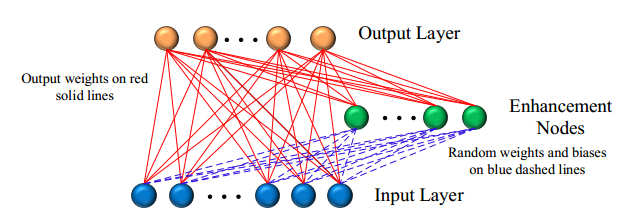
\includegraphics[width=0.75\textwidth]{RVFL20181102Sys.PNG}
  \caption{The architecture of the RVFL network.}
  \label{RVFLNN181102Sys}
\end{figure}
%%%%%%%%%%%%%%%%%%%%%%%%%%%

The RVFL+ is an unified learning algorithm for all binary, multiclass classification and regression, and the output function in (19) can be straightforwardly applied for all three
cases. \index{Classification and regression}\index{Regression and Classification}
\begin{enumerate}
  \item Binary Classification: The predicted label of the test
sample is determined by
\begin{align}
  \hat y = \textup{sign}(f_{test}(z))
\end{align}
  \item Multiclass Classification: We adopt the one-vs.-all (OvA) strategy to determine the predicted label in the multiclass classification. Let $f_{test}^k (z)$ be the output function of the k-th output nodes. The predicted label of the test sample is determined by
\begin{align}
  \hat y = \arg \max_{ k \in 1,\cdots,m} f_{test}^k (z)
\end{align}
  \item  Regression: The predicted value is equal to the output function $f_{test}(z)$ of the RVFL+
\begin{align}
  \hat y = f_{test}(z)
\end{align}
\end{enumerate}

Following the formula of the SVM+ in \cite{VAPNIK2009544}, we can write the RVFL+ as
\begin{align}
&\min\limits_{{\bm w},\tilde {\bm w}} \frac 1 2 \|{\bm w}\|_2^ 2 + \frac \gamma 2 \|\tilde {\bm w}\|_2^ 2 + C\sum_{i=1}^N \zeta_i (\tilde {\bm w}, {\tilde h}({\tilde {\bm x}}_i))\notag\\
&s.t.\,\, \bm h(\tilde x_i){\bm w} = \bm y_i - \zeta_i (\tilde {\bm w}; {\tilde h}({\tilde {\bm x}}_i)), \forall \leq i \leq  N.\label{RVFL20181102eq8}
\end{align}
where $\gamma$ is a regularization coefficient. Likewise to $\bm h(\bm x_i)$, ${\tilde {\bm h}}({\tilde {\bm x}}_i)$ is also an enhanced layer output vector corresponding to the privileged feature ${\tilde {\bm x}}_i$, which can be calculated in the same fashion. $\zeta_i (\tilde {\bm w}, {\tilde h}({\tilde {\bm x}}_i))$ is the correcting function (or slack function) in the privileged feature space, and $\tilde {\bm w}$ is an output weight vector for the correcting function.
\begin{align}\label{RVFL20181102eq9}
\zeta_i (\tilde {\bm w}, {\tilde h}({\tilde {\bm x}}_i)) = {\tilde h}({\tilde {\bm x}}_i){\bm w}
\end{align}

Substituting \eqref{RVFL20181102eq9} into \eqref{RVFL20181102eq8}, we have the primal form of the RVFL+ as follows.
\begin{align}
&\min\limits_{{\bm w},\tilde {\bm w}} \frac 1 2\|{\bm w}\|_2^ 2 + \frac \gamma 2 \|\tilde {\bm w}\|_2^ 2 + C\sum_{i=1}^N  {\tilde {\bm h}}({\bm x}_i)\tilde {\bm w}\notag\\
&s.t.\,\,\bm h(\tilde x_i){\bm w} =\bm y_i - {\tilde {\bm h}}({\bm x}_i)\tilde {\bm w}, \forall \leq i \leq  N.\label{RVFL20181102eq10}
\end{align}
From \eqref{RVFL20181102eq10}, we note that the RVFL+ minimizes the objective function over both w and w~. Therefore, Not only the original features but also the privileged information determine meanwhile the separating hyperplane of the RVFL+ during the training stage.

Moreover, in contrasts to the primal form of the SVM+ in \cite{VAPNIK2009544}, the correcting function of the RVFL+ is either positive or negative. In other words, the RVFL+ does not consider a group of constraints $\zeta_i(\tilde {\bm h}, b, \phi({\bm x}_i)) \geq 0 (i = 1,\cdots,N)$. As a result, the number of constraints in the RVFL+ is at least N less than that of the SVM+ for the binary classification, which results that the RVFL+ has much milder optimization constraints than the SVM+.

Furthermore, in order to address the optimization problem in \eqref{RVFL20181102eq10}, we construct the Lagrangian function $\mathscr L (\bm w, \tilde{\bm w},\bm \lambda)$ as
\begin{align}
\min\limits_{\bm w, \tilde{\bm w},\bm \lambda} \frac 1 2\|{\bm w}\|_2^ 2 + \frac \gamma 2 \|\tilde {\bm w}\|_2^ 2 + C\sum_{i=1}^N  {\tilde {\bm h}}({\bm x}_i)\tilde {\bm w}-\sum_{i=1}^N  \bm \lambda_i(\bm h(\tilde {\bm x}_i){\bm w} -\bm y_i +{\tilde {\bm h}}({\bm x}_i)\tilde {\bm w}),
\end{align}
where $\bm \lambda = [\bm \lambda_1,\cdots, \bm \lambda_N]^T$ are Lagrange multipliers. To find solutions, we use the KKT condition to calculate the saddle points of the Lagrangian function $\mathscr L (\bm w, \tilde{\bm w},\bm \lambda)$ with respect to $\bm w, \tilde{\bm w}$ and $\bm \lambda$.
\begin{align}
 &\frac {\partial \mathscr L (\bm w, \tilde{\bm w},\bm \lambda)}{\partial \bm w}= 0 \Rightarrow  \bm w = \bm  H^T \bm \lambda, \label{RVFL20181102eq12}\\
 &\frac {\partial \mathscr L (\bm w, \tilde{\bm w},\bm \lambda)}{\partial \tilde{\bm w}} = 0 \Rightarrow  \tilde{\bm w} = \frac 1  \gamma  (\tilde{\bm  H}^T  \bm \lambda - \tilde{\bm  H}^T C \bm 1), \label{RVFL20181102eq13}\\
 &\frac {\partial \mathscr L (\bm w, \tilde{\bm w},\bm \lambda)}{\partial \bm \lambda_i} = 0 \Rightarrow  \bm h(\bm x_i)\bm w - \bm y_i + \tilde {\bm h}({\bm x}_i) \tilde{\bm w} = 0, 1 \leq  i \leq  N.\label{RVFL20181102eq14}
\end{align}
where $\bm 1 \in \mathbb R^{N\times m}$ is an identify matrix. $\tilde {\bm H}$ is also a concatenated output matrix from the enhancement nodes, which corresponds to the privileged features.

Substituting \eqref{RVFL20181102eq12} and \eqref{RVFL20181102eq13} into \eqref{RVFL20181102eq14}, we have
\begin{align}
  \bm H \bm H^T  \bm \lambda + \frac 1 \gamma\tilde{\bm H} \tilde{\bm H}^T  (\bm \lambda -C \bm 1) = \bm Y \label{RVFL20181102eq15}
\end{align}

We can further reformulate \eqref{RVFL20181102eq15} as
\begin{align}
  \left(\bm H \bm H^T  + \frac 1 \gamma \tilde{\bm H} \tilde{\bm H}^T \right )\bm \lambda  = \bm Y - \frac {C \bm 1} {\gamma}\tilde{\bm H} \tilde{\bm H}^T  \label{RVFL20181102eq16}
\end{align}
Combining \eqref{RVFL20181102eq12} and \eqref{RVFL20181102eq16}, we obtain the closed-form solution to the RVFL+ as follows.
\begin{align}
\bm  w =\bm H^T \left(\bm H \bm H^T  + \frac 1 \gamma \tilde{\bm H} \tilde{\bm H}^T \right )^{-1} \left(\bm Y - \frac {C \bm 1} {\gamma}\tilde{\bm H} \tilde{\bm H}^T \right ) \label{RVFL20181102eq17}
\end{align}
According to the ridge regression \cite{Bishop2012-6469}, we also impose an additional term $\frac {\bm I} C $ in order to avoid singularity and guarantee the stability of the RVFL+. As a result, we can achieve the aftermost closed-form solution to the RVFL+ as
\begin{align}
\bm w = \bm H^T \left(\bm H \bm H^T  + \frac 1 \gamma \tilde{\bm H} \tilde{\bm H}^T +\frac{ \bm I} C \right)^{-1} \left(\bm Y -\frac {C \bm 1} {\gamma}\tilde{\bm H} \tilde{\bm H}^T \right )
\label{RVFL20181102eq18}
\end{align}
Consequently, the output function of the RVFL+ is defined as
\begin{align}
  f(x) =\bm  h (\bm x)\bm w =\bm h(\bm  x)\bm H^ T \left(\bm H \bm H^T  +\frac 1 \gamma\tilde{\bm H} \tilde{\bm H}^T  +\frac{\bm  I} C \right)^{-1}\left(\bm Y - \frac {C \bm 1} {\gamma}\tilde{\bm H} \tilde{\bm H}^T \right ).
\end{align}
In addition, we can obtain straightforwardly the output function $f_{test}(\bm z) = \bm h(\bm z)\bm w$ in the test stage, when using the test data z instead of the training data $\bm x$.
\subsubsection{区间二型模糊集}
本节将随机向量函数链接网络(RVFL) 推广到了张量结构,  增强节点使用了区间二型模糊集来扩展非线性激活函数, 主要目的是用二型模糊集来捕捉输入输出关系中蕴含的高阶信息.
提出了两种随机向量函数链接网络, 一种是区间二型随机向量函数链接网络, 另一种是基于张量的二型随机向量函数链接网络.
区间二型随机向量函数链接网络和随机向量函数链接网络类似, 不同之处在于 其输出增强节点的输出是不确定加权方法的解模糊结果.
张量的二型随机向量函数链接网络也使用了不确定加权方法, 同时还使用了下隶属函数值和上隶属函数值, 由此形成了一个 4阶张量.
基于这个结构, 基于Einstein积的偶数阶张量的Moore-Penrose逆被用来求解张量方程.
此外, 权重向量由一个平衡因子综合得到, 它是RVFL网络结果和张量方程结果的加权平均.
最后, 分别在三个非线性测试函数、非线性系统识别问题和四个回归问题上验证了给出的算法.


高斯区间二型模糊集有两种定义形式,  不确定均值或者是不确定方差. 本节使用的区间二型模糊集上隶属和下隶属的均值相同.  图 \ref{TFLN:fig1-2}  给出了均值相同、方差不同的区间二型模糊集. 隶属函数按如下的方式定义
%%%%%%%%%%%%%%%%%%%%%%%%%%%%%
\begin{figure} [!htp]
\begin{center}
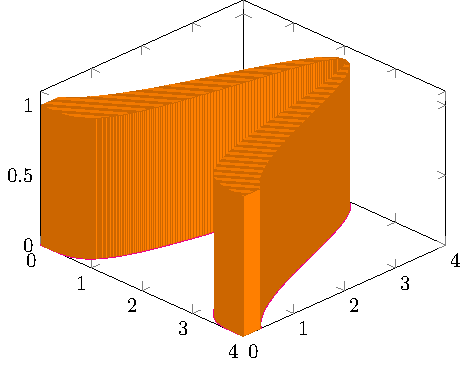
\includegraphics[width =0.6\linewidth]{IntervalT2MF}
\end{center}
\caption{区间二型模糊集}
\label{TFLN:fig1-2}
\end{figure}
%%%%%%%%%%%%%%%%%%%%%%%%%%%%%%%
\begin{align}
  &\bar{\mu} _{i} (x_i)=\exp\left(- \frac{(x_i-m_{i} )^2} {\bar{\sigma} ^2_{i} }  \right),\label{IT2TSKNM_mu1} \\
  &\underline{\mu} _{i} (x_i)=\exp\left(- \frac{(x_i-m_{i} )^2} {\underline{\sigma} ^2_{i} }  \right),\label{IT2TSKNM_mu2}
\end{align}
其中 $m_{i} $, $\bar{\sigma} _{i} $ 和 $\underline{\sigma} _{i} $ $(1\leq i\leq L)$ 分别是二型模糊集的下隶属函数和上隶属函数的均值和方差 . 下隶属函数和上隶属函数之间的隶属度是1的二型模糊集就是区间二型模糊集.

图 \ref{TensorRVFL20180927-2} 给出了基于张量积的区间二型随机向量函数链接网络 (TT2-RVFL), 其中 $\tilde g_i(\cdot)\, (i=1,2,\cdots,L)$ 是区间二型模糊激活函数. 不同于RVFL, TT2-RVFL使用区间二型模糊集, 扩展了RVFL的增强节点部分,
因此, 区间二型模糊集的输出可以看成是原来两个激活函数的输出结果. RVFL网络中的乘法需要修正, 对于高维结构的TT2-RVFL, 增强型节点使用了张量的Einstein积运算.
%%%%%%%%%%%%%%%%%%%%%%%%%%%%%%%%%%%%%%%%%%%%%%%%%%%%%%%%%%%%%%
%The functional link net and learning optimal control, 1995, \cite{PaoPhillips1995-36113}
\begin{figure} [!htbp]
\def\circlrad2{0.1}
\begin{center}
\begin{tikzpicture} [scale=0.8,>=stealth,rotate border/.style={shape border uses incircle, shape border rotate=#1} ]
% layer 1
 \node(layer01) at (2,1) {$x_{1} $} ;
 \node(layer02) at (3.8,1) {$x_{l} $} ;
 \node(layer03) at (5,1) {$x_{L} $} ;
 \node(layer04) at (7,1) {\footnotesize $\tilde g_1(\bm a_1 \bm x_1+b_1)$} ;
 \node(layer05) at (9.8,1) {\footnotesize $\tilde g_2(\bm a_l \bm x_l+b_l)$} ;
 \node(layer06) at (12.8,1) {\footnotesize $\tilde g_L(\bm a_L \bm x_L+b_L)$} ;
% layer 2
 \node(layer11) at (2,3) {} ;
 \node(layer12) at (3.8,3) {} ;
 \node(layer13) at (5,3) {} ;
 \node(layer14) at (7,3) {} ;
 \node(layer15) at (9.8,3) {} ;
 \node(layer16) at (12.8,3) {} ;
%  cdots
 \node(layer1cd) at (2.9,3) {$\cdots$} ;
 \node(layer1cd) at (4.45,3) {$\cdots$} ;

 \node(layer1cd) at (8.75,3) {$\cdots$} ;
 \node(layer1cd) at (11,3) {$\cdots$} ;

\draw[fill=blue!30] (layer11) circle (\circlrad2 cm) node[xshift=0.1cm,yshift=0.2cm,above] {$w_1$} ;
\draw[fill=blue!30] (layer12) circle (\circlrad2 cm) node[xshift=0.1cm,yshift=0.2cm,above] {$w_l$} ;
\draw[fill=blue!30] (layer13) circle (\circlrad2 cm) node[xshift=0.75cm,yshift=0.2cm,above] {$w_L$} ;
\draw[fill=blue!30] (layer14) circle (\circlrad2 cm) node[xshift=0.65cm,yshift=0.2cm,above] {$\bm w_{L+1} $} ;;
\draw[fill=blue!30] (layer15) circle (\circlrad2 cm) node[xshift=0.1cm,yshift=0.2cm,above] {$\bm w_{2l} $} ;
\draw[fill=blue!30] (layer16) circle (\circlrad2 cm) node[xshift=0.1cm,yshift=0.2cm,above] {$\bm w_{2L} $} ;

% layer 3
\node(layer21) at (7.5,6) {} ;
\draw[fill=blue!40] (layer21) circle (\circlrad2 cm);

% layer 4
\node(layer31) at (7.5,7) {} ;
\draw[->] ($(layer21)+(0,\circlrad2)$) -- (layer31);

% 0->1
%\draw[->] ($(layer01) +(0.2,0)$) -- ($(layer11)-(0.6,0.1)$);
\draw[->] (layer01) -- ($(layer11)-(0,\circlrad2)$);
\draw[->] (layer02) -- ($(layer12)-(0,\circlrad2)$);
\draw[->] (layer03) -- ($(layer13)-(0,\circlrad2)$);
\draw[->,thick=1.2] (layer04) -- ($(layer14)-(0,\circlrad2)$);
\draw[->,thick=1.2] (layer05) -- ($(layer15)-(0,\circlrad2)$);
\draw[->,thick=1.2] (layer06) -- ($(layer16)-(0,\circlrad2)$);
% 1->2
\draw[->] ($(layer11)+(0,\circlrad2)$)--($(layer21)-(0,\circlrad2)$);
\draw[->] ($(layer12)+(0,\circlrad2)$)--($(layer21)-(0,\circlrad2)$);
\draw[->] ($(layer13)+(0,\circlrad2)$)--($(layer21)-(0,\circlrad2)$);
\draw[->,thick=1.2] ($(layer14)+(0,\circlrad2)$)--($(layer21)-(0,\circlrad2)$);
\draw[->,thick=1.2] ($(layer15)+(0,\circlrad2)$)--($(layer21)-(0,\circlrad2)$);
\draw[->,thick=1.2] ($(layer16)+(0,\circlrad2)$)--($(layer21)-(0,\circlrad2)$);
% y
\node(layery) at (7.5,7.05) {$\bm Y$} ;
\end{tikzpicture}
\caption{TT2-RVFL的结构}
\label{TensorRVFL20180927-2}
\end{center}
\end{figure}
%%%%%%%%%%%%%%%%%%%%%%%%%%%%%%%%%%%%%%%%%%%%%%%%%%
TT2-RVFL 的输出模型如图 \ref{TensorRVFL20180927-2}:
\begin{align}
  \bm Y=\mathcal A *_N \mathcal X+\bm H \bm \Omega,\label{TensorRVFLEq05}
\end{align}
其中 $\mathcal A *_N \mathcal X$ 为增强节点的张量乘积, $\bm H \bm \Omega$ 为线性部分的输出 ,  $\mathcal X$ 为增强节点部分的权重矩阵;
类似于RVFL, $\bm H$ 是输入数据矩阵, 单列输出的数据需要复制一次, 以便与张量和矩阵的运算结果相容, $\Omega$是线性部分的权矩阵, 且$\mathcal A$是一个张量, 它是由 叠加区间二型模糊集的映射结果得到的张量.
对于TT2-RVFL, $\bm Y$, $\mathcal X$ 和$\Omega$需要特别考虑, 以便和后件形成的张量方程相容. 下一节将介绍由三个变量组成的张量结构.
%%%%%%%%%%%%%%%%%%%%%%%%%%%%%%%%%%%%%%%%%%%%%%%%%%%%%%%%%%%%
\subsubsection{TT2-RVFL} {TT2-RVFL}
RVFL常使用 Radbas ($y = \exp(-s^2)$), Sine ($y = \textup{sine} (s)$), Sigmoid ($y = \frac 1 {1+e^{-s} } $) 和Tribas ($y = \max(1 - |s|, 0)$)这几类激活函数,其中 $s$ 和 $y$分别表示输入和输出变量.
对于TT2-RVFL, 增强节点使用了区间二型模糊集. RVFL的 Radbas激活函数被 推广成区间二型模糊集, 扩展后的 RVFL 使用了区间二型模糊集, 扩展后的激活函数简记为 IT2Radbas, 它是 \eqref{IT2TSKNM_mu1} 和 \eqref{IT2TSKNM_mu2} 的变种,  记为$\tilde g_i(\cdot)$, 可以用下面的式子表示为
 \begin{align}
  &\bar{g} _{i} (x_i)=\exp(-k_1 s^2),\label{IT2TSKNM_g1} \\
  &\underline{g} _{i} (x_i)=\exp(-k_2 s^2),\label{IT2TSKNM_g2}
\end{align}
其中 $s=x_i-m_{i} , k_1=\frac{1} {\bar{\sigma} ^2_{i} } $, $k_2=\frac{1} {\underline{\sigma} ^2_{i} } \, (i=1,2,\cdots, L)$.

对于测试集$\{D_t\} _{t=1} ^{N} $, 其中 $D_t=(\bm x_t,y_t)$, $\bm x_t=(x_{t1} ,x_{t2} ,\cdots,x_{tN} )\in \mathbb R^{N} $, $y_t\in \mathbb R$ 且$\bm y=[y_1,\cdots, y_N]^T$. 下隶属函数矩阵 $\underline\Phi\in \mathbb R^{N\times 2\times L \times 1} $可用下式构建
\begin{align*}
\begin{array} {cc}
 \underline\Phi_{:,:,1,1}  =\begin{bmatrix}
  \underline g_1(\bm {a} _{11}  \bm x_1+b_{11} )&\underline g_1(\bm {a} _{12}  \bm x_1+b_{12} )\\
   \vdots&\vdots\\
  \underline g_1(\bm {a} _{11}  \bm x_N+b_{11} )&\underline g_1(\bm {a} _{12}  \bm x_N+b_{12} )
\end{bmatrix},\\
\vdots\\
   \underline\Phi_{:,:,L,1}  =\begin{bmatrix}
  \underline g_L(\bm {a} _{L1}  \bm x_1+b_{L1} )&\underline g_L(\bm {a} _{L2}  \bm x_1+b_{L2} )\\
   \vdots&\vdots\\
  \underline g_L(\bm {a} _{L1}  \bm x_N+b_{L1} )&\underline g_L(\bm {a} _{L2}  \bm x_N+b_{L2} )
\end{bmatrix},
\end{array}
\end{align*}
其中 $b_{il} $和$\bm {a} _{il} =[w_{i1} ,w_{i2} 、,\cdots,w_{iK} ]$ ($i=1, 2, \cdots, L$; $l=1,2$) 是随机生成的偏置和输入权重. 下隶属函数矩阵使用下隶属函数来逼近输入$\bm x_t$ 和期望输出$y_t$的关系.
上隶属函数矩阵$\bar \Phi\in \mathbb R^{N\times 2\times L \times 1}$ 可以用类似的方式建立, 具有如下形式
\begin{align*}
 \begin{array} {cc}
 \bar\Phi_{:,:,1,2}  =\begin{bmatrix}
  \bar g_1(\bm {a} _{11}  \bm x_1+b_{11} )&\bar g_1(\bm {a} _{12}  \bm x_1+b_{12} )\\
   \vdots&\vdots\\
  \bar g_1(\bm {a} _{11}  \bm x_N+b_{11} )&\bar g_1(\bm {a} _{12}  \bm x_N+b_{12} )
\end{bmatrix},\\
\vdots\\
   \bar\Phi_{:,:,L,2}  =\begin{bmatrix}
  \bar g_L(\bm {a} _{L1}  \bm x_1+b_{L1} )&\bar g_L(\bm {a} _{L2}  \bm x_1+b_{L2} )\\
   \vdots&\vdots\\
  \bar g_L(\bm {a} _{L1}  \bm x_N+b_{L1} )&\bar g_L(\bm {a} _{L2}  \bm x_N+b_{L2} )
\end{bmatrix},
\end{array}
\end{align*}
其中 $\bm {a} _{ij} \,(i=1,2\cdots,L; j=1,2)$是构建张量所用的随机生成的权重向量.
%%%%%%%%%%%%%%%%%%%%%%%%%%%%%%%%%%%%%%%%
\begin{remark}
不确定加权方法\cite{RunklerCoupland2018-6356}  被用于区间二型模糊激活函数的解模糊化计算,
它代表了隶属函数隶属度对于整体解模糊化结果的影响程度, 映射结果由下式计算得到
\begin{align} \label{TensorRVFLEq08}
  u_{UW} (x) =\frac 1 2 (\underline u(x) + \bar u(x))\cdot (1+\underline u(x)-\bar u(x))^\gamma,
\end{align}
其中 $\gamma > 0$ 用于调整由$(1+\underline u(x)-\bar u(x))^\gamma$给出解模糊化结果.
不确定加权方法推广了简单的平均下隶属和上隶属度方法, 清晰输出结果由下式给出
\begin{align} \label{TensorRVFLEq09}
  (1+\underline u(x)-\bar u(x))^\gamma=
  \left\{
  \begin{array} {ll}
    0,& \underline u(x)=0, \bar u(x)=1,\\
    1,&\underline u(x)=\bar u(x).\\
  \end{array}
  \right.
\end{align}
方程 \eqref{TensorRVFLEq09} 显示出: 当$\gamma =1$时, 解模糊结构呈线性, 对于所有的 $\gamma<1$ 线性增加, 且对于所有 $\gamma>1$, 线性性将会减少.
\end{remark}
%%%%%%%%%%%%%%%%%%%%%%%%%%%%%%%%%%%%%%%%
\begin{remark}
当 \eqref{TensorRVFLEq09} 被用于解模糊化, 只用区间二型模糊集拓展随机向量函数链接网络, 也即,  只是扩展了原网络的增强节点为区间二型模糊集,  这种类型的网络记为IT2-RVFL.
\end{remark}

最后得到的 4阶张量$\Upphi \in \mathbb R^{N\times 2\times L \times 2} $ 是由前面提到的张量$\underline\Phi_{:,:,:,1} $和$\bar \Phi_{:,:,:,2} $构建出来的.
接下来, 张量$\Upphi$用$\mathcal A$来记,  这是由于经典的张量方程中经常使用$\mathcal A$表示张量方程的系数.

基于张量的乘积运算, 得到的增强节点的权重矩阵 维数是$L \times 2$, 将TT2-RVFL的增强节点部分的权重矩阵记为
\begin{align}
  \mathcal X=
  \begin{bmatrix}
    \bm {w} _{L+1\, 1} &\bm {w} _{L+1\,  2} \\
    \bm {w} _{L+2\, 1} &\bm {w} _{L+2\,  2} \\
    \vdots &\vdots\\
    \bm {w} _{2L\, 1} &\bm {w} _{2L\,  2}
  \end{bmatrix} .
\end{align}
TT2-RVFL 的输出可用下式表示
\begin{align}
  \bm Y=\alpha\mathcal A *_N \mathcal X+(1-\alpha)\bm H \bm \Omega, 0\leq \alpha\leq 1,\label{TensorRVFLEq08}
\end{align}
其中 $\alpha$是TT2-RVFL的平衡因子, $\mathcal A$是区间二型模糊激活函数的映射结果, $\mathcal X$是权重矩阵, $\bm Y=[\bm y\, \bm y]$, 从输入到增强节点的权重向量$\bm {a} _{i} \,(i=1,2,\cdots, L)$是随机生成的,  使得 $\underline\Phi$, $\bar\Phi$不饱和;  $\bm\Omega=[\bm \omega\, \bm \omega]$是待求的输入权重矩阵,  $\bm H$ 是由输入样本构建的输入矩阵.
%%%%%%%%%%%%%%%%%%%%%%%%%%%%%%%%%%%%%%%%%%%%%
\begin{remark}
  当下三角隶属函数和上三角隶属函数一样时, TT2-RVFL 退化为RVFL, 也即, 激活函数是一型模糊集. 当不适用直接连接方式,  TT2-RVFL 将会退化为张量型极限学习机 \cite{HuangZhao2018NCAA-5838}. 当同时使用RVFL和张量结构时,  TT2-RVFL是这两种结构的混合结果.
\end{remark}
%%%%%%%%%%%%%%%%%%%%%%%%%%%%%%%%%%%%%%%%%%%%%
%%%%%%%%%%%%%%%%%%%%%%%%%%%%%%%%%%%%%%%%%%%%%
\begin{remark}
  和RVFL相比, 基于张量的二型 RVFL模型 \eqref{TensorRVFLEq08} 做了三方面的扩展: 1) 增强节点使用区间二型模糊激活函数来得到非线性映射结果, 增强节点部分由张量和张量乘法表示, 且使用了张量方程的求解算法 .  2) 为了和增强节点的运算相容, TT2-RVFL的线性部分需要 复制权重向量一次, 权重矩阵 $\bm\Omega$等于 $[\bm \omega\, \bm \omega]$, 其中 $\bm \omega$为权重列向量.  3) 对于输出$\bm Y$, 和以前的输出向量 $\bm y$不同, TT2-RVFL需要重复该向量一次, 以便和张量运算相容.
\end{remark}
%%%%%%%%%%%%%%%%%%%%%%%%%%%%%%%%%%%%%%%%%%%%%
%%%%%%%%%%%%%%%%%%%%%%%%%%%%%%%%%%%%%%%%%%%%%%%%%%%%%%%%%%%%%
%\begin{algorithm} [!ht]
%\caption{偶数阶张量$\mathcal A$的M-P逆 \cite{HuangZhao2018NCAA-5838}}
%\label{T2RVFL3:alg1}
%\begin{algorithmic} [1] %
%\REQUIRE 输入: 张量$\mathcal A$, $I_{1 \cdots N} $ 和指标 $J_{1 \cdots N} $.
%\ENSURE $N$ 为偶数, $I=\prod_{i=1} ^N I_i$, $J=\prod_{i=1} ^N J_i$.
%\STATE 变换张量$\mathcal A\in \mathbb R^{I_{1 \cdots N} \times J_{1 \cdots N} } $ 为矩阵 $A\in \mathbb R^{I\times J} $.
%\STATE 对矩阵$A$做奇异值分解, $A$ 可以分解为 $A=U S V^*$, 其中 $V^*$ 是矩阵$V$的共轭转置.
%\STATE 分别将矩阵$U, S$和$V^*$ 转换为相应阶次的张量$\mathcal U, \mathcal S$ 和$\mathcal V^*$.
%\STATE 输出: 通过$\mathcal A^+ = \mathcal V *_N\mathcal S^+ *_N \mathcal U^*$计算张量$\mathcal A$的 M-P逆.
% \end{algorithmic}
%\end{algorithm}
%%%%%%%%%%%%%%%%%%%%%%%%%%%%%%%%%%%%%%%%%%%%%%%%%%%%%%%%%%%%
%%%%%%%%%%%%%%%%%%%%%%%%%%%%%%%%%%%%%%%%%%%%%%%%%%%%%%%%%%%%%%%%%%%%%%%%%%%%%%%%%%%%%%%%%%%%%%%%%%%
\subsubsection{TT2-RVFL中的张量逆} \label{Trapezoidsection5-1}
张量方程 $\mathcal A *_N \mathcal X = \mathcal Y$的张量运算被用于求解 TT2-RVFL网络的权重向量,  该运算非常适合计算TT2-RVFL增强节点部分的权重向量.
求解方程使用的偶数阶张量的 Moore-Penrose (M-P)逆在算法 \ref{T2RVFL3:alg1} 中给出,  在得到M-P逆的基础上, 可以很容易算出权重矩阵.
%%%%%%%%%%%%%%%%%%%%%%%%%%%%%%%%%%%%%%%%%%%%%%%%%%%%%%%%%%%%
\begin{remark}
方程$\mathcal A *_N \mathcal X = \mathcal Y$的解也是如下张量方程的解
\begin{align}
  \mathcal A^T *_N\mathcal  A *_N \mathcal X = \mathcal A^T *_N \mathcal Y,
\end{align}
其中张量$\mathcal A \in \mathbb R^{I_1\times \cdots\times I_N\times J_1\times \cdots\times J_N} $, $\mathcal X \in \mathbb R^{J_1\times \cdots\times J_N\times K_1\times \cdots\times K_M} $且 $\mathcal Y \in \mathbb R^{I_1\times \cdots\times I_N\times K_1\times \cdots\times K_M} $, 不论方程是否相容, 都可以应用算法 \ref{T2RVFL3:alg1} 来求解方程 $\mathcal  A *_N \mathcal X = \mathcal Y$ \cite{HuangZhao2018NCAA-5838}.
\end{remark}
%%%%%%%%%%%%%%%%%%%%%%%%%%%%%%%%%%%%%%%%%%%%%%%%%%%
\subsubsection{求解TT2-RVFL的张量逆算法} {Tensor inverse algorithms for solving the TT2-RVFL} \label{Trapezoidsection5-2}
为了得到TT2-RVFL的解,  模型 \eqref{TensorRVFLEq08} 的最小范目标函数定义为
\begin{align} \label{TensorRVFLEq13}
  \min_{\bm \Omega,\mathcal X}  \mathcal E_1(\mathcal X)+ \mathcal E_2( \Omega),
\end{align}
其中 $\mathcal E_1(\mathcal X)=\| \bm Y -\mathcal A \mathcal X \|_F^2+\|\mathcal X \|_F^2$, $\mathcal E_2(\Omega)=\|\bm y-\bm H \bm \Omega\|_2^2+\|\bm \Omega\|_2^2$.
模型 \eqref{TensorRVFLEq08} 的极小化问题可以划分成两个子问题来求解, 由下面的定理给出:
%%%%%%%%%%%%%%%%%%%%%%%%%%%%%%%%%%%%%%%%%%%%%%%
\begin{mythm}{极小化模型的解}{1}
 对于极小化模型 \eqref{TensorRVFLEq08}, 令$\Omega^*$ 是$\bm y= \bm H \bm \Omega$的解集, $\mathcal X^*$ 是$\mathcal Y=\mathcal A *_N \mathcal X$的解.
 对于模型 \eqref{TensorRVFLEq13} 的两个子问题$\mathcal E_1(\mathcal X)$ 和 $\mathcal E_2(\mathcal X)$, $\mathcal Y$ 退化为一个矩阵, 即$\mathcal Y=[\bm y\, \bm y]$,
 且$\bm y$是训练结果列向量. 式 \eqref{TensorRVFLEq08} 的充分条件就是寻找如下子问题的解
\begin{align}
  \min_{\mathcal X}  \mathcal E_1(\mathcal X)\, \textup{和} \, \min_{\bm \Omega} \mathcal E_2(\Omega),\label{TensorRVFLEq11}
\end{align}
则方程的解 $\begin{bmatrix}  \mathcal X & \bm \Omega \end{bmatrix} ^T$ 满足下式
\begin{align}
  \bm Y=\mathcal A *_N \mathcal X+\bm H \bm \Omega=
  \begin{bmatrix}
    \mathcal A& \bm H
  \end{bmatrix}
  *
  \begin{bmatrix}
    \mathcal X\\
    \bm \Omega
  \end{bmatrix} ,\\
    \begin{bmatrix}
    \mathcal X\\
    \bm \Omega
  \end{bmatrix}
  =\begin{bmatrix}
    \alpha \mathcal X^*\\
    (1-\alpha)\bm \Omega^*
  \end{bmatrix} ,
\end{align}
其中 $\alpha$是 TT2-RVFL ($0\leq \alpha\leq 1$)的平衡因子, $*_N$是张量$\mathcal A$和$\mathcal X$的Einstein乘积.
\end{mythm}
\begin{proof}
  $\bm H \bm \Omega=\bm Y$的解是$\Omega^*$, $\bm H \bm \Omega^*=\bm Y$成立.
  $\mathcal X^*$ 是$\mathcal A *_N \mathcal X=\mathcal Y$的解, 则$\mathcal A *_N \mathcal X^*=\mathcal Y$.
  给定平衡因子$\alpha$, $\mathcal A *_N  \alpha \mathcal X^*+\bm H (1-\alpha)\bm \Omega^*=\alpha \bm Y+(1-\alpha)\bm Y=\bm Y$成立.
  对于$\bm Y\equiv \mathcal Y$的情况, 张量$\mathcal Y$ 退化为矩阵$\bm Y$, 且$\bm Y\in \mathbb R^{L\times 2}$.
\end{proof}
%%%%%%%%%%%%%%%%%%%%%%%%%%%%%%%%%%%%%%%%%%%%%%%
%%%%%%%%%%%%%%%%%%%%%%%%%%%%%%%%%%%%%%%%%%%%%%%%%%%%%%%%%%%%
\begin{remark}
  对于TT2-RVFL, 权重向量是RVFL的输出结果和 张量方程解结果的综合, RVFL的权重向量记为$\bm \omega=(\bm H^T \bm H+\frac {\bm I}  C)^{-1} \bm H^T \bm Y$, 其中 $\bm I$ 是单位矩阵, 且 $C$ 是平衡参数.
\end{remark}

%%%%%%%%%%%%%%%%%%%%%%%%%%%%%%%%%%%%%%%%%%%%%
\subsubsection{仿真实验} \label{TensorFLNsection4}
提出的算法使用了Frobenius 范数来度量训练误差和测试误差,  所有结果都由1000次运行结果求得. 为了说明IT2-RVFl 和 TT2-RVFL的学习能力, 隐藏节点数选为$L=[30,35,40]$.
IT2-RVFL 和 TT2-RVFL使用了均值一样, 方差不确定这一形式, 下隶属函数从区间$[0.5,0.9]$随机选取, 上隶属函数通过给下隶属函数值加 0.1 得到; 则$k_1, k_2$ 可由关系式$k_1=\frac{1} {\bar{\sigma} ^2_{i}}, k_2=\frac{1} {\underline{\sigma} ^2_{i}} \,(i=1,2,\cdots, L)$ 求得.
%$\bar{q} $ is the average of $q_1, \cdots, q_N$
\subsubsection{非线性函数}

%%%%%%%%%%%%%%%%%%%%%%%%%%%%%%%%%%%%%%%%%%%%%%%%例-1
\textbf{例 4.1}: 单输入 Sinc 函数的逼近问题如下
\begin{align}
  y =\left\{
  \begin{array} {ll}
    1, &x = 0 \\
    \frac{\sin\,x} {x} ,&x\neq 0
  \end{array} \right. x\in[-10,10].
\end{align}
对于 IT2RVFL和 TT2-RVFL, 平衡参数设置为$C=2^{10} $, $\gamma =0.95$.
表 \ref{TT2-RVFL181123:Sec4-1} 给出了例 4.1在不同 $L$下的训练误差和测试误差.
对于IT2-RVFL, 当$L=30,35$, 它的训练误差要小于TT2-RVFL的训练误差. 然而,  TT2-RVFL 的测试误差要小于IT2-RVFL的测试误差,  这意味着TT2-RVFL中的平衡因子对网络的学习能力有一定的影响.
%%%%%%%%%%%%%%%%%%%%%%%%%%%%%%%%%%%%%%%%%%%%%%%%%%%%%%%%%%%%%%%%%%%%%%%%%%%%%%%%table 1
\begin{table} [!ht]
\caption{例 4.1中不同$L$下的训练和测试误差 } \label{TT2-RVFL181123:Sec4-1}
\vspace{-0.4cm}
\begin{center}
\begin{tabular} {p{0.25cm} p{2.75cm} ccccccc}
\hline
\multirow{2} {*} {$L$} &\multirow{2} {*} {算法} &\multicolumn{2} {c} {训练误差} &\multicolumn{2} {c} {预测误差} \\
\cline{3-4} \cline{5-6}
&&  均值   &  方差 &  均值   &  方差 \\
\hline
\multirow{2} {*} {30}   &IT2-RVFL&2.53e-02  & 4.51e-05 &  4.82e-02  & 7.22e-04\\
     &TT2-RVFL&   \textbf{2.36e-04}  &  \textbf{1.71e-05}  &  \textbf{2.32e-04}  &  \textbf{1.70e-05} \\
\multirow{2} {*} {35}   &IT2-RVFL&   2.34e-02 &  9.15e-05 &  4.66e-02 &  3.17e-04\\
     &TT2-RVFL&   \textbf{1.57e-02}  &  \textbf{7.44e-05}  &  \textbf{1.54e-02}   & \textbf{7.61e-05} \\
\multirow{2} {*} {40}   &IT2-RVFL&   \textbf{2.18e-02}  &  \textbf{1.38e-04}   & 4.57e-02 &  7.92e-04\\
     &TT2-RVFL&   3.86e-02 &  4.25e-04  & \textbf{3.76e-02}   & \textbf{4.25e-04} \\
\hline
\end{tabular}
\end{center}
\end{table}
%%%%%%%%%%%%%%%%%%%%%%%%%%%%%%%

%%%%%%%%%%%%%%%%%%%%%%%%%%%%%%%%%%%%%%%%%%%%%%%%例-2
\textbf{例 4.2}: 含噪的非线性函数具有如下形式
\begin{align} \label{nonlinearfunctioneq17}
  y=\frac{0.9x} {1.2x^3+x+0.3} +\eta,x\in[0,1],
\end{align}
其中 $\eta$ 是均匀分布的白噪声,  $\eta$的幅值设置为 0.2.

例 4.2用来测试给出算法的野值拒绝能力.
对于IT2RVFL和 TT2-RVFL, 平衡参数设置为$C=2^{10} $, $\gamma =1$.
表 \ref{TT2-RVFL181121:Sec4-2} 给出了例4.2在不同$L$值下的训练误差和测试误差.
结果表明, 当$L=30,35,40$时, TT2-RVFL 性能要好于 IT2-RVFL,  其平均训练误差和测试误差要小于IT2-RVFL的结果.
%%%%%%%%%%%%%%%%%%%%%%%%%%%%%%%%%%%%%%%%%%%%%%%%%%%%%%%%%%%%%%%%%%%%%%%%%%%%%%%%table 2
\begin{table} [!ht]
\caption{例 4.2中不同$L$下的训练误差和预测误差}
\vspace{-0.4cm}
\begin{center}
 \begin{tabular} {p{0.25cm} p{2.75cm} cccc}
\hline
\multirow{2} {*} {$L$} &\multirow{2} {*} {算法} &\multicolumn{2} {c} {训练误差} &\multicolumn{2} {c} {预测误差} \\
\cline{3-4} \cline{5-6}
&&  均值   &  方差 &  均值   &  方差 \\
\hline
\multirow{2} {*} {30}   &IT2-RVFL&2.85e-01 &  \textbf{7.30e-06}  &  4.13e-01 &  5.58e-03\\
     &TT2-RVFL&\textbf{2.07e-01}   & 8.43e-04  & \textbf{3.07e-01}  &  \textbf{2.19e-03} \\
\multirow{2} {*} {35}   &IT2-RVFL&2.85e-01 &  \textbf{2.94e-06}   & 4.15e-01 &  2.45e-03\\
     &TT2-RVFL&\textbf{2.07e-01}   & 1.75e-03  & \textbf{3.06e-01}  &  \textbf{1.96e-03} \\
\multirow{2} {*} {40}   &IT2-RVFL& 2.85e-01 &  \textbf{5.14e-06}   & 4.11e-01 &  5.10e-03\\
     &TT2-RVFL&\textbf{2.06e-01}   & 4.54e-04  & \textbf{3.04e-01}  & \textbf{1.13e-03} \\
\hline
\end{tabular}
\end{center}
\label{TT2-RVFL181121:Sec4-2}
\end{table}
%%%%%%%%%%%%%%%%%%%%%%%%%%%%%%%

%%%%%%%%%%%%%%%%%%%%%%%%%%%%%%%%%%%%%%%%%%%%%%%%例-3
\textbf{例 4.3}: 双输入单输出 Sinc函数的逼近问题.
\begin{align} \label{two-inputSincfun}
 z =\left|\frac{\sin x\cdot\sin y} {x y} \right|, (x,y)\in [-\pi,\pi]^2.
\end{align}
采用等距采样方式, $41\times 41$ 训练数据对用于训练, $30\times 30$等距采样结果用来检验模型的泛化能力.
对于IT2-RVFL和TT2-RVFL, 平衡因子设置为 $C=2^{10} $, $\gamma =1$.
表 \ref{TT2-RVFL181121:Sec4-3} 给出了例4.3在不同$L$下的训练误差和测试误差.
\begin{figure}
  \centering
  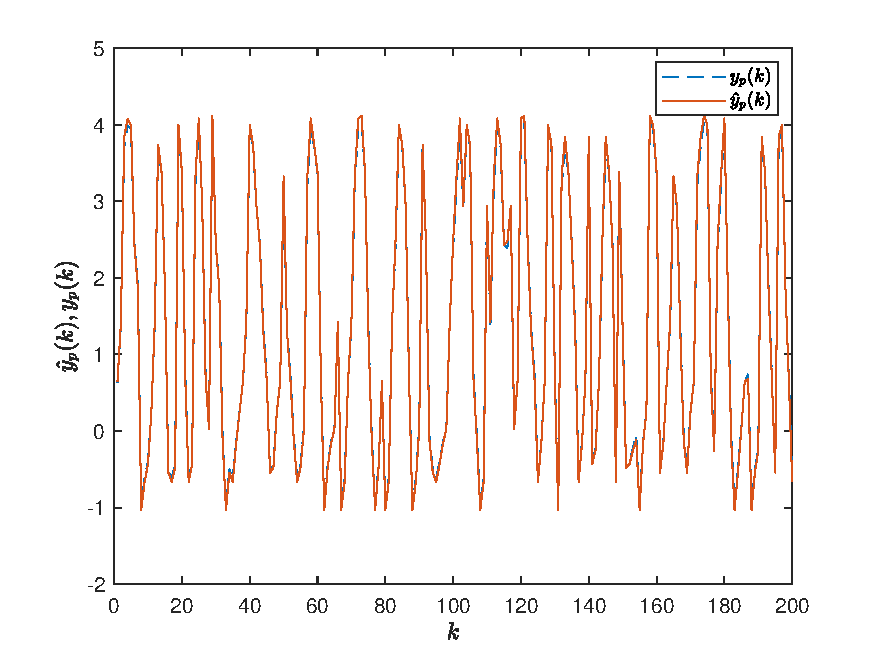
\includegraphics[width=0.6\textwidth]{nonlinearfunTstRslutsT2RVFL.pdf}
   \caption{TT2-RVFL对非线性系统识别问题的预测结果}
  \label{nonlinearfunTstRslutsT2RVFL-fig4}
\end{figure}
TT2-RVFL的结果要好于 IT2-RVFL的结果, 训练误差和测试误差都要小于IT2-RVFL的结果.
%%%%%%%%%%%%%%%%%%%%%%%%%%%%%%%%%%%%%%%%%%%%%%%%%%%%%%%%%%%%%%%%%%%%%%%%%%%%%%%table 3
\begin{table} [!ht]
\caption{例 4.3中不同$L$下的训练误差和预测误差}
\vspace{-0.4cm}
\begin{center}
 \begin{tabular} {p{0.25cm} p{2.75cm} cccc}
\hline
\multirow{2} {*} {$L$} &\multirow{2} {*} {算法} &\multicolumn{2} {c} {训练误差} &\multicolumn{2} {c} {预测误差} \\
\cline{3-4} \cline{5-6}
&&  均值   &  方差 &  均值   &  方差 \\
\hline
\multirow{2} {*} {30}   &IT2-RVFL& 4.65e-02  & \textbf{3.09e-06}   & 7.06e-02  & \textbf{1.43e-09} \\
     &TT2-RVFL&   \textbf{4.36e-02}   & 1.30e-05 &  \textbf{6.77e-02}  &  6.05e-06\\
\multirow{2} {*} {35}   &IT2-RVFL&   4.63e-02 &  \textbf{8.69e-06}  &  7.06e-02  & \textbf{2.40e-08} \\
     &TT2-RVFL&   \textbf{4.07e-02}   & 3.38e-05 &  \textbf{6.73e-02}   & 9.21e-06\\
\multirow{2} {*} {40}   &IT2-RVFL&   \textbf{4.63e-02}  &  \textbf{2.95e-06}  &  7.06e-02  & \textbf{1.56e-09} \\
     &TT2-RVFL&   \textbf{3.98e-02}   & 4.72e-05  & \textbf{6.75e-02}  &  1.09e-05\\
\hline
\end{tabular}
\end{center}
\label{TT2-RVFL181121:Sec4-3}
\end{table}
%%%%%%%%%%%%%%%%%%%%%%%%%%%%%%%
%%%%%%%%%%%%%%%%%%%%%%%%%%%%%%%%%%%%%%%%%%%%%%%%%%%%%%%%%%%%%%%%%%%%%%%%%%%%%%%%%%%%%%%%%%%%%%%%
\subsubsection{非线性系统参数识别}
对于如下的非线性系统 \cite{Rong2009-4804697}
\begin{align} \label{TT2FS:Nonlinearsys18}
  y_p(k) =\frac{ y_p(k - 1)y_p(k - 2)(y_p(k - 1) + 2.5)} {1 + (y_p(k - 1))^2 + (y_p(k - 2))^2}  + u(k - 1).
\end{align}
系统的平衡态为 (0,0),  输入 $u(k) \in \{-2, 2\} $, 操作区间规定为 $[-2, 2]$. 均匀分布的随机变量从$\{-2, 2\}$ 中产生,  测试使用的输入 $u(k) = \sin(2\pi k/25)$.
通过选取$[y_p(k - 1), y_p(k - 2), u(k - 1)]$作为输入变量,  $y_p(k)$作为输出变量. 系统可以写为
\begin{align}
 \hat y _p(k) = \hat f(y_p(k - 1), y_p(k - 2), u(k - 1)).
\end{align}
随机选用了800组数据, 600 组用于训练,  200 组用于测试.
对于IT2RVFL 和 TT2-RVFL, 平衡参数设置为$C=2^{10}$.
对于仿真,  TT2-RVFL 的预测结果见图 \ref{nonlinearfunTstRslutsT2RVFL-fig4}.
训练误差均值的Frobenius 范数 是1.87e-01, 测试误差均值的Frobenius 范数 是3.94e-01,  结果显示,  TT2-RVFL能够得到满意的精度.
%%%%%%%%%%%%%%%%%%%%%%%%%%%%%%%%%%%%%%%
\subsubsection{回归问题} {Regression problems}
%%%%%%%%%%%%%%%%%%%%%%%%%%%%%%%%%%%%%%%%%%%%%%%%%%%%%%%%%%%%%%%%%%%%%%%%%%%%%%%%
\begin{table} [H]
\caption{数据集 Auto-Mpg, Bank, Diabetes 和 Triazines上的训练和测试误差}
\vspace{-0.4cm}
\begin{center}
 \begin{tabular} {llccccccccc}
\hline
\multirow{2} {*} {数据集} &\multirow{2} {*} {算法} &\multicolumn{2} {c} {训练误差} &\multicolumn{2} {c} {预测误差} \\
\cline{3-4} \cline{5-6}
&&  均值   &  方差  &  均值   &  方差   \\
\hline
\multirow{5} {*} {Auto-Mpg} &ELM   &4.3511e-01   &2.4125e+0   &4.3423e-01   &2.5502e+0   \\
&RELM   &1.3514e+0   &1.6125e+0   &1.3132e+0   &1.6101e+0   \\
&RVFL & 9.9152e-01 &  6.3012e-03   &9.2356e-01  & 5.1511e-03\\
&IT2-RVFL&\textbf{2.2161e-02}   & \textbf{1.5915e-04}   & 4.5358e-02  & \textbf{1.6692e-04}  \\
&TT2-RVFL&4.4055e-02  & 8.1940e-04  & \textbf{4.3847e-02}   & 8.1024e-04\\
\cline{3-6}
%%%%%%%%--------------------------------------
\multirow{5} {*} {Bank} &ELM    &3.2400e-02   &5.8710e-02  &3.2103e-02   &5.8425e-02\\
&RELM    &3.3214e-02   &5.8321e-02      &\textbf{3.0936e-02}    &5.8631e-02\\
&RVFL &1.1784e-01 &  6.3033e-03  & 5.0163e-02 &  1.3696e-04\\
&IT2-RVFL&\textbf{2.9035e-02}   & \textbf{3.4437e-05}   & 7.0701e-02 &  9.9726e-05\\
&TT2-RVFL&4.3582e-02 &  1.1435e-04 &  5.1382e-02 &  \textbf{8.3401e-05} \\
\cline{3-6}
%%%%%%%%--------------------------------------
\multirow{5} {*} {Diabetes} &ELM  &1.5199e-01   &1.5535e-01   &1.5724e-01   &1.3706e-01  \\
&RELM   &1.5046e-01   &1.3448e-01   &1.5741e-01   &1.4002e-01 \\
&RVFL &3.3931e-01  & 6.2734e-02   &\textbf{8.6827e-02}  &  1.0573e-02\\
&IT2-RVFL&1.4838e-01  & 2.6181e-05  & 1.5938e-01  & 4.3915e-04\\
&TT2-RVFL&\textbf{1.4548e-01}  &  \textbf{2.1532e-06}   & 1.4522e-01  & \textbf{8.8627e-05} \\
\cline{3-6}
%%%%%%%%--------------------------------------
\multirow{5} {*} {Triazines} &ELM &9.8322e-02   &2.4095e-01   &1.0947e-01   &1.6613e-01   \\
&RELM    &9.9402e-02   &2.1026e-01   &1.0739e-01   &1.6718e-01\\
&RVFL &3.0201e-01 &  2.8114e-01  & \textbf{2.2935e-02}   & 1.3741e-02\\
&IT2-RVFL&\textbf{8.2873e-02}  &  \textbf{6.5574e-05}  &  4.0105e-01  & 3.9270e-03\\
&TT2-RVFL&1.0360e-01  & 3.1127e-04 &  2.6182e-01 &  \textbf{1.0300e-03} \\
\hline
\end{tabular}
\end{center}
\label{TT2-RVFL181116:Sec4-1}
\end{table}
%%%%%%%%%%%%%%%%%%%%%%%%%%%%%%%
测试使用了四个回归数据集 (Auto-Mpg, Bank, Diabetes 和  Triazines).
Auto-MPG 数据集有392 个样本, 每一个样本有 8 个属性.   Bank数据集有8192个样本, 每一个样本有 8 个属性.
Diabetes 数据集有768个样本, 每一个样本有4个属性.  Triazines 数据集有186个样本, 每一个样本有5个属性.
对于Auto-MPG 和 Bank, 使用了mapminmax 方法来计算映射到区间 $[-1,1]$ 的数据.
而对于Diabetes和Triazines, 则直接使用原来的数据样本.
对于IT2-RVFL和 TT2-RVFL, 平衡参数设置为 $C=2^{10}$, $\gamma =1$.
RVFL的代码可以从Matlab的File Exchange下载,  ELM 和RELM 的代码可以从\href{https://www.ntu.edu.sg/home/egbhuang/elm_random_hidden_nodes.html}{主页下载}.
表 \ref{TT2-RVFL181116:Sec4-1} 给出了ELM、RELM、RVFL、IT2-RVFL和TT2-RVFL算法的训练误差和测试误差.
对于Auto-MPG, 扩展后的RVFL的训练误差和测试误差都得到了很好的结果.
IT2-RVFL在Bank上的训练误差最小,  RELM在Bank上的测试误差最小, 这说明正则化项在ELM的训练过程中是发挥作用的.
TT2-RVFL 在Diabetes上的训练误差最小, 它的测试误差要大于 RVFL, 均值的误差大约是0.0584.
IT2-RVFL 在Triazines 的训练误差最小, 而RVFL的测试误差则总体较小.
对于四个数据集的回归结果, 可以得出 IT2-RVFL和 TT2-RVFL是可以作为回归问题的求解器使用的.
如表 \ref{TT2-RVFL181121:Sec4-2} 的结果所示, TT2-RVFL更适合于数据含噪的情形.
%%%%%%%%%%%%%%%%%%%%%%%%%%%%%%%%%%%%%%
\section{进化计算}
进化计算(Evolutionary Computation,EC)是在达尔文(Darwin)的进化论和孟德尔(Mendel)的遗传变异理论的基础上产生的一种在基因和种群层次上模拟自然界生物进化过程与机制的问题求解技术.
神经进化是人工智能和机器学习领域的一个分支, 是一种机器学习技术, 它能够改进了人工神经网络, 并且试图通过进化算法去寻找最优神经网络. 具体而言, 就像大自然通过突变、交叉或移除一些潜在的遗传密码来提高大脑的功能一样, 人工神经网络通过进化算法能够产生越来越好的拓扑、权重和超参数. 简单的说就是将进化的思想使用到神经网络参数优化的更迭中. 它使用基于群体的优化方法能够不断提高群体中每个神经网络的质量, 从而根据其要解决的问题生成越来越好的神经网络. 该种群中的每个个体的存储方式并不是复杂的神经网络, 而是存储为基因组. 基因组是一种简化的遗传表示, 可以映射到神经网络.
%%%%%%%%%%%%%%%%%%%%%%%%%%%%%%%%%%%%
\begin{figure}[H]
\centering
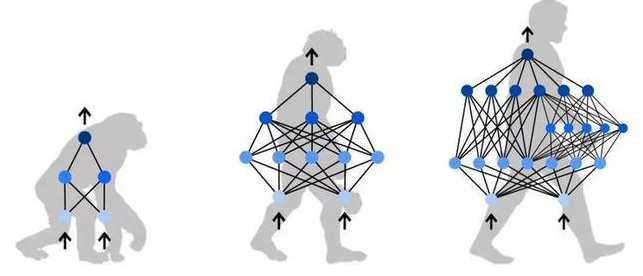
\includegraphics[width=0.85\textwidth]{NetEvolving2020020401.png}
\caption{神经进化演化过程}
\label{NetEvolving2020020401}
\end{figure}

进化计算主要包括
%%%%%%%%%%%%%%%%%%%%%%%%%%%%%%%%%%%%%%%%%%
\begin{itemize}
\item 遗传算法(Genetic Algorithm, GA)
\item 进化策略(Evolutionary Strategy, ES)
\item 进化规划(Evolutionary Programming, EP)
\item 遗传规划(Genetic Programming,GP)四大分支.
\end{itemize}
其中, 第一个分支是进化计算中最初形成的一种具有普遍影响的模拟进化优化算法. 因此我们主要讨论遗传算法.

进化计算是一种模拟自然界生物进化过程与机制进行问题求解的自组织、自适应的随机搜索技术. 它以达尔文进化论的“物竟天择、适者生存”作为算法的进化规则, 并结合孟德尔的遗传变异理论, 将生物进化过程中的
%%%%%%%%%%%%%%%%%%%%%%%%%%%%%%%%%%%%%%%%%%
\begin{itemize}
\item 繁殖(Reproduction)
\item 变异(Mutation)
\item 竞争(Competition)
\item 选择(Selection)
\end{itemize}
引入到了算法中.

  (2) 进化计算的生物学基础

  自然界生物进化过程是进化计算的生物学基础, 它主要包括遗传(Heredity)、变异(Mutation)和进化(Evolution)理论.

  \ding{172} 遗传理论

  遗传是指父代(或亲代)利用遗传基因将自身的基因信息传递给下一代(或子代), 使子代能够继承其父代的特征或性状的这种生命现象. 正是由于遗传的作用, 自然界才能有稳定的物种.

  在自然界, 构成生物基本结构与功能的单位是细胞(Cell). 细胞中含有一种包含着所有遗传信息的复杂而又微小的丝状化合物, 人们称其为染色体(Chromosome).
  在染色体中, 遗传信息由基因(Gene)所组成, 基因决定着生物的性状, 是遗传的基本单位.
   染色体的形状是一种双螺旋结构, 构成染色体的主要物质叫做脱氧核糖核酸(DNA), 每个基因都在DNA长链中占有一定的位置.
   一个细胞中的所有染色体所携带的遗传信息的全体称为一个基因组(Genome).
   细胞在分裂过程中, 其遗传物质DNA通过复制转移到新生细胞中, 从而实现了生物的遗传功能.

   \ding{173} 变异理论

   变异是指子代和父代之间, 以及子代的各个不同个体之间产生差异的现象. 变异是生物进化过程中发生的一种随机现象, 是一种不可逆过程, 在生物多样性方面具有不可替代的作用. 引起变异的主要原因有以下两种:
   杂交, 是指有性生殖生物在繁殖下一代时两个同源染色体之间的交配重组, 即两个染色体在某一相同处的DNA被切断后再进行交配重组, 形成两个新的染色体. 复制差错, 是指在细胞复制过程中因DNA上某些基因结构的随机改变而产生出新的染色体.

    \ding{174}  进化论

    进化是指在生物延续生存过程中, 逐渐适应其生存环境, 使得其品质不断得到改良的这种生命现象. 遗传和变异是生物进化的两种基本现象, 优胜劣汰、适者生存是生物进化的基本规律.

    达尔文的自然选择学说认为: 在生物进化中, 一种基因有可能发生变异而产生出另一种新的生物基因. 这种新基因将依据其与生存环境的适应性而决定其增殖能力. 一般情况下, 适应性强的基因会不断增多, 而适应性差的基因则会逐渐减少. 通过这种自然选择, 物种将逐渐向适应于生存环境的方向进化, 甚至会演变成为另一个新的物种, 而那些不适应于环境的物种将会逐渐被淘汰.
%%%%%%%%%%%%%%%%%%%%%%%%%%%%%%
\subsection{进化计算的产生与发展}
 进化计算自20世纪50年代以来, 其发展过程大致可分为三个阶段.

     \ding{172}  萌芽阶段

     这一阶段是从20世纪50年代后期到70年代中期. 20世纪50年代后期, 一些生物学家在研究如何用计算机模拟生物遗传系统中, 产生了遗传算法的基本思想, 并于1962年由美国密执安(Michigan)大学霍兰德(Holland)提出. 1965年德国数学家雷切伯格(Rechenberg)等人提出了一种只有单个个体参与进化, 并且仅有变异这一种进化操作的进化策略. 同年, 美国学者弗格尔(Fogel)提出了一种具有多个个体和仅有变异一种进化操作的进化规划. 1969年美国密执安(Michigan)大学的霍兰德(Holland)提出了系统本身和外部环境相互协调的遗传算法. 至此, 进化计算的三大分支基本形成.

    \ding{173}  成长阶段

     这一阶段是从20世纪70年代中期到80年代后期. 1975年, 霍兰德出版专著《自然和人工系统的适应性(Adaptation in Natural and Artificial System)》, 全面介绍了遗传算法. 同年, 德国学者施韦费尔(Schwefel)在其博士论文中提出了一种由多个个体组成的群体参与进化的, 并且包括了变异和重组这两种进化操作的进化策略. 1989年, 霍兰德的学生戈尔德伯格(Goldberg)博士出版专著《遗传算法----搜索、优化及机器学习(Genetic Algorithm----in Search Optimization and Machine Learning)》, 使遗传算法得到了普及与推广.

   \ding{174}  发展阶段

     这一阶段是从20世纪90年代至今. 1989年, 美国斯坦福(Stanford)大学的科扎(Koza)提出了遗传规划的新概念, 并于1992年出版了专著《遗传规划----应用自然选择法则的计算机程序设计(Genetic Programming:on the Programming of Computer by Means of Natural Selection)》该书全面介绍了遗传规划的基本原理及应用实例, 标志着遗传规划作为计算智能的一个分支已基本形成.

    进入20世纪90年代以来, 进化计算得到了众多研究机构和学者的高度重视, 新的研究成果不断出现、应用领域不断扩大. 目前, 进化计算已成为人工智能领域的又一个新的研究热点.

%%%%%%%%%%%%%%%%%%%%%%%%%%%%%%
\subsection{进化计算的基本结构}
进化计算尽管有多个重要分支, 并且不同分支的编码方案、选择策略和进化操作也有可能不同, 但它们却有着共同的进化框架. 若假设$P$为种群(Population, 或称为群体), $t$为进化代数,  $P(t)$为第$t$代种群 , 则进化计算的基本结构可粗略描述如下:
\begin{Verbatim}
{确定编码形式并生成搜索空间;
   初始化各个进化参数, 并设置进化代数$t=0$;
   初始化种群$P(0)$;
   对初始种群进行评价(即适应度计算);
   while(不满足终止条件)do
       {
       $t=t+1$;
       利用选择操作从$P(t-1)$代中选出$P(t)$代群体;
       对$P(t)$代种群执行进化操作;
       对执行完进化操作后的种群进行评价(即适应度计算);
       }
}
\end{Verbatim}

可以看出, 上述基本结构包含了生物进化中所必需的选择操作、进化操作和适应度评价等过程.

遗传算法的基本思想是从初始种群出发, 采用优胜劣汰、适者生存的自然法则选择个体, 并通过杂交、变异来产生新一代种群, 如此逐代进化, 直到满足目标为止. 遗传算法所涉及到的基本概念主要有以下几个:
%%%%%%%%%%%%%%%%%%%%%%%%%%%%%%%%%%%%%%%%%%
\begin{itemize}
\item 种群(Population): 种群是指用遗传算法求解问题时, 初始给定的多个解的集合. 遗传算法的求解过程是从这个子集开始的.
\item 个体(Individual): 个体是指种群中的单个元素, 它通常由一个用于描述其基本遗传结构的数据结构来表示. 例如, 可以用0、1组成的长度为l的串来表示个体.
\item 染色体(Chromos): 染色体是指对个体进行编码后所得到的编码串. 染色体中的每1位称为基因, 染色体上由若干个基因构成的一个有效信息段称为基因组.
\item 适应度(Fitness)函数: 适应度函数是一种用来对种群中各个个体的环境适应性进行度量的函数. 其函数值是遗传算法实现优胜劣汰的主要依据
\item 遗传操作(Genetic Operator): 遗传操作是指作用于种群而产生新的种群的操作. 标准的遗传操作包括以下3种基本形式:
\item 选择(Selection)
\item 交叉(Crosssover)
\item 变异(Mutation)
\end{itemize}

遗传算法主要由染色体编码、初始种群设定、适应度函数设定、遗传操作设计等几大部分所组成, 其算法主要内容和基本步骤可描述如下:

(1) 选择编码策略, 将问题搜索空间中每个可能的点用相应的编码策略表示出来, 即形成染色体;

(2) 定义遗传策略, 包括种群规模$N$, 交叉、变异方法, 以及选择概率$P_r$、交叉概率$P_c$、变异概率$P_m$等遗传参数;

(3) 令$t=0$, 随机选择$N$个染色体初始化种群$P(0)$;

(4) 定义适应度函数$f(f>0)$;

(5) 计算$P(t)$中每个染色体的适应值;

(6) $t=t+1$;

(7) 运用选择算子, 从$P(t-1)$中得到$P(t)$;

(8) 对$P(t)$中的每个染色体, 按概率$P_c$参与交叉;

(9) 对染色体中的基因, 以概率$P_m$参与变异运算;

(10) 判断群体性能是否满足预先设定的终止标准, 若不满足则返回(5).

其算法流程如图\ref{AI32fig2019120226518}所示.
%%%%%%%%%%%%%%%%%%%%%%%%%%%%%%%%%%%%%%%%%%
\begin{figure}[H]
\centering
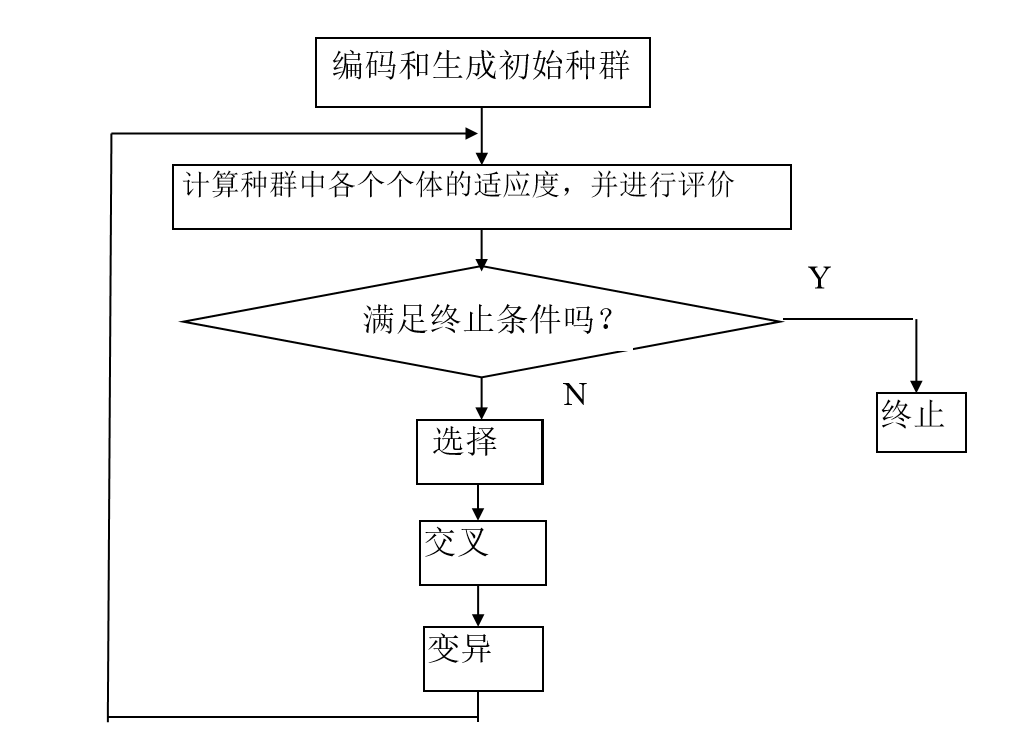
\includegraphics[width=0.76\textwidth]{AI32C420191126518.PNG}
\caption{}
\label{AI32fig2019120226518}
\end{figure}
%%%%%%%%%%%%%%%%%%%%%%%%%%%%%%%%%%%%%%%%%%
%%%%%%%%%%%%%%%%%%%%%%%%%%%%%%
\section{遗传编码}

常用的遗传编码算法有霍兰德二进制码、格雷码(Gray Code)、实数编码和字符编码等.

(1)二进制编码(Binary encoding)

二进制编码是将原问题的结构变换为染色体的位串结构. 在二进制编码中, 首先要确定二进制字符串的长度l, 该长度与变量的定义域和所求问题的计算精度有关.
%%%%%%%%%%%%%%%%%%%%%%%%%%%%%%%%%
\begin{example}
假设变量$x\in [5,10]$, 要求的计算精度为$10^{-5}$, 则需要将[5, 10]至少分为600000个等长小区间, 每个小区间用一个二进制串表示. 于是, 串长至少等于20, 原因是:
\begin{align*}
  524288=2^{19}<600000<2^{20}=1048576
\end{align*}
这样, 对应于区间$[5,10]$内满足精度要求的每个值$x$, 都可用一个20位编码的二进制串$<b_{19},b_{18},\cdots,b_0>$来表示.
\end{example}

二进制编码存在的主要缺点是汉明(Hamming)悬崖.

%%%%%%%%%%%%%%%%%%%%%%%%%%%%%%%%%
\begin{example}
  7和8的二进制数分别为0111和1000, 当算法从7改进到8时, 就必须改变所有的位.
\end{example}

 (2) 格雷编码(Gray encoding)

格雷编码是对二进制编码进行变换后所得到的一种编码方法. 这种编码方法要求两个连续整数的编码之间只能有一个码位不同, 其余码位都是完全相同的. 它有效地解决了汉明悬崖问题, 其基本原理如下:

设有二进制串$b_1,b_2,\cdots,b_n$, 对应的格雷串为$a_1,a_2,\cdots,a_n$, 则从二进制编码到格雷编码的变换为:

\begin{align}
  a_{i}=\left\{\begin{array}{ll}{b_{1},} & {i=1} \\ {b_{i-1} \oplus b_{i}} & {i>1}\end{array}\right.
\end{align}
其中, ⊕表示模2加法. 而从一个格雷串到二进制串的变换为:
\begin{align}
  b_{i}=\sum_{j=1}^{i} a_{i}(\bmod 2)
\end{align}
%%%%%%%%%%%%%%%%%%%%%%%%%%%%%%%%%%%%%%%%%%%%
\begin{example}
  十进制数7和8的二进制编码分别为0111和1000, 而其格雷编码分别为0100和1100.
\end{example}

 (3) 实数编码(Real encoding)


实数编码是将每个个体的染色体都用某一范围的一个实数(浮点数)来表示, 其编码长度等于该问题变量的个数.

这种编码方法是将问题的解空间映射到实数空间上, 然后在实数空间上进行遗传操作. 由于实数编码使用的是变量的真实值, 因此这种编码方法也叫做真值编码方法.

实数编码适应于那种多维、高精度要求的连续函数优化问题.

适应度函数是一个用于对个体的适应性进行度量的函数. 通常, 一个个体的适应度值越大, 它被遗传到下一代种群中的概率也就越大.

(1) 常用的适应度函数


 在遗传算法中, 有许多计算适应度的方法, 其中最常用的适应度函数有以下两种:

\ding{172} 原始适应度函数

 它是直接将待求解问题的目标函数$f(x)$定义为遗传算法的适应度函数. 例如, 在求解极值问题
\begin{align}
 \max _{x \in[a, b]} f(x)
\end{align}
时, $f(x)$即为$x$的原始适应度函数.

采用原始适应度函数的优点是能够直接反映出待求解问题的最初求解目标, 其缺点是有可能出现适应度值为负的情况.

\ding{173} 标准适应度函数

在遗传算法中, 一般要求适应度函数非负, 并其适应度值越大越好. 这就往往需要对原始适应函数进行某种变换, 将其转换为标准的度量方式, 以满足进化操作的要求, 这样所得到的适应度函数被称为标准适应度函数$f_{\textup{Normal}}(x)$.
%%%%%%%%%%%%%%%%%%%%%%%%%%%%%%%%%
\paragraph{极小化问题}
对极小化问题, 其标准适应度函数可定义为
\begin{align}
f(x)=
\left\{\begin{array}{ll}
{f_{\max }(x)-f(x)} &f(x)<f_{\max}(x) \\
{0} & f(x)\geq f_{\max }(x)
\end{array}
\right.
\end{align}
其中, $f_{\max}(x)$是原始适应函数$f(x)$的一个上界. 如果$f_{\max}(x)$未知, 则可用当前代或到目前为止各演化代中的$f(x)$的最大值来代替. 可见,  $f_{\max}(x)$是会随着进化代数的增加而不断变化的.
%%%%%%%%%%%%%%%%%%%%%%%%%%%%%%%%%
\paragraph{极大化问题}
对极大化问题, 其标准适应度函数可定义为
\begin{align}
  f(x)=\left\{
  \begin{array}{ll}
  f(x)-f_{\min }(x) &f(x)>f_{\min}(x)\\
 0 & f(x)\leq f_{\min}(x)
  \end{array}
  \right.
\end{align}
其中, $f_{\min}(x)$是原始适应函数$f(x)$的一个下界. 如果$f_{\min}(x)$未知, 则可用当前代或到目前为止各演化代中的$f(x)$的最小值来代替.

(2) 适应度函数的加速变换

在某些情况下, 适应度函数在极值附近的变化可能会非常小, 以至于不同个体的适应值非常接近, 使得难以区分出哪个染色体更占优势. 对此, 最好能定义新的适应度函数, 使该适应度函数既与问题的目标函数具有相同的变化趋势, 又有更快的变化速度.

适应度函数的加速变换有两种基本方法

\ding{172} 线性加速

适应度函数的定义如下:
\begin{align}
  f'(x)=\alpha f(x)+\beta
\end{align}
其中, $f(x)$是加速转换前的适应度函数; $f'(x)$是加速转换后的适应度函数;  $\alpha$和$\beta$是转换系数.

    \ding{173}  非线性加速
%%%%%%%%%%%%%%%%%%%%%%%%%%%%%%%%%
\begin{itemize}
\item 幂函数变换方法
   \begin{align}
     f'(x)=f(x)k
   \end{align}
\item 指数变换方法
         \begin{align}
           f'(x)=exp^{-\beta f(x)}
         \end{align}
\end{itemize}

遗传算法中的基本遗传操作包括选择、交叉和变异3种, 而每种操作又包括多种不同的方法, 下面分别对它们进行介绍.

%%%%%%%%%%%%%%%%%%%%%%%%%%%%%%%%%
\begin{itemize}
\item 选择操作

   选择(Selection)操作是指根据选择概率按某种策略从当前种群中挑选出一定数目的个体, 使它们能够有更多的机会被遗传到下一代中.

    常用的选择策略可分为比例选择、排序选择和竞技选择三种类型.

\item 比例选择

    比例选择方法(Proportional Model)的基本思想是: 各个个体被选中的概率与其适应度大小成正比.

    常用的比例选择策略包括: (1) 轮盘赌选择. (2)繁殖池选择

\item 轮盘赌选择

    轮盘赌选择法又被称为转盘赌选择法或轮盘选择法. 在这种方法中, 个体被选中的概率取决于该个体的相对适应度. 而相对适应度的定义为:
\begin{align}
  P\left(x_{i}\right)=\frac{f\left(x_{i}\right)}{\sum_{j=1}^{N} f\left(x_{j}\right)}
\end{align}
其中, $P(x_i)$是个体$x_i$的相对适应度, 即个体$x_i$被选中的概率; $f(x_i)$是个体$x_i$的原始适应度; 是种群的累加适应度.
\end{itemize}
轮盘赌选择算法的基本思想是: 根据每个个体的选择概率$P(x_i)$将一个圆盘分成$N$个扇区, 其中第$i$个扇区的中心角为:
\begin{align}
  2 \pi \frac{f\left(x_{i}\right)}{\sum_{j=1}^{N} f_{i}\left(x_{j}\right)}=2 \pi p\left(x_{i}\right)
\end{align}

并再设立一个固定指针. 当进行选择时, 可以假想转动圆盘, 若圆盘静止时指针指向第$i$个扇区, 则选择个体$i$. 其物理意义如图5-19所示.

从统计角度看, 个体的适应度值越大, 其对应的扇区的面积越大, 被选中的可能性也越大. 这种方法有点类似于发放奖品使用的轮盘, 并带有某种赌博的意思, 因此亦被称为\textbf{轮盘赌选择}.

(2)交叉操作

交叉(Crossover)操作是指按照某种方式对选择的父代个体的染色体的部分基因进行交配重组, 从而形成新的个体. 交配重组是自然界中生物遗传进化的一个主要环节, 也是遗传算法中产生新的个体的最主要方法. 根据个体编码方法的不同, 遗传算法中的交叉操作可分为二进制交叉和实值交叉两种类型.

    \ding{172} 二进制交叉

    二进制交叉(Binary Valued Crossover)是指二进制编码情况下所采用的交叉操作, 它主要包括单点交叉、两点交叉、多点交叉和均匀交叉等方法.


    \ding{173} 单点交叉

    单点交叉也称简单交叉, 它是先在两个父代个体的编码串中随机设定一个交叉点, 然后对这两个父代个体交叉点前面或后面部分的基因进行交换, 并生成子代中的两个新的个体. 假设两个父代的个体串分别是:
\begin{align}
    X&=x_1 x_2 \cdots x_k\, x_{k+1} \cdots x_n\\
    Y&=y_1 y_2 \cdots y_k\,  y_{k+1} \cdots y_n
\end{align}

    随机选择第$k$位为交叉点, 若采用对交叉点后面的基因进行交换的方法, 但点交叉是将X中的$x_{k+1}$到$x_n$部分与$Y$中的$y_{k+1}$到$y_n$部分进行交叉, 交叉后生成的两个新的个体是:
\begin{align}
    X'&= x_1 x_2 \cdots x_k y_{k+1} \cdots y_n\\
    Y'&= y_1 y_2 \cdots y_k x_{k+1} \cdots x_n
\end{align}
%%%%%%%%%%%%%%%%%%%%%%%%%%%%%
\begin{example}
设有两个父代的个体串$A=0\, 0\,  1\,  1\,  0\,  1$和$B=1\,  1\,  0\,  0\,  1\,  0$, 若随机交叉点为4, 则交叉后生成的两个新的个体是:
\begin{align}
    A'= 0\, 0\, 1\, 1\, 1\, 0\\
    B'= 1\, 1\, 0\, 0\, 0\, 1
\end{align}
\end{example}

    \ding{174} 两点交叉

两点交叉是指先在两个父代个体的编码串中随机设定两个交叉点, 然后再按这两个交叉点进行部分基因交换, 生成子代中的两个新的个体.

假设两个父代的个体串分别是:
\begin{align}
    X&=x_1\, x_2 \cdots x_i \cdots x_j \cdots x_n\\
    Y&=y_1\, y_2 \cdots y_i \cdots y_j \cdots y_n
\end{align}

随机设定第$i,j$位为两个交叉点(其中$i<j<n$), 两点交叉是将$X$中的$x_{i+1}$到$x_j$部分与$Y$中的$y_{i+1}$到$y_j$部分进行交换, 交叉后生成的两个新的个体是:
\begin{align}
  X'&= x_1\, x_2 \cdots x_i\, y_{i+1} \cdots y_j\, x_{j+1} \cdots x_n\\
  Y'&= y_1\, y_2  \cdots y_i\, x_{i+1} \cdots x_j\, y_{j+1} \cdots y_n
\end{align}

%%%%%%%%%%%%%%%%%%%%%%%%%%%%%
\begin{example}
设有两个父代的个体串$A= 0\, 0\,  1\,  1\,  0\,  1$和B=$1\,  1\,  0\,  0\,  1\,  0$, 若随机交叉点为3和5, 则交叉后的两个新的个体是:
\begin{align}
  A'&= 0 0 1 0 1 1\\
  B'&= 1 1 0 1 0 0
\end{align}
\end{example}

    \ding{175} 多点交叉

多点交是指先随机生成多个交叉点, 然后再按这些交叉点分段地进行部分基因交换, 生成子代中的两个新的个体.

假设交叉点个数为$m$, 则可将个体串划分为$m+1$个分段, 其划分方法是:

当$m$为偶数时, 对全部交叉点依次进行两两配对, 构成$m/2$个交叉段.

当$m$为奇数时, 对前$(m-1)$个交叉点依次进行两两配对, 构成$(m-1)/2$个交叉段, 而第$m$个交叉点则按单点交叉方法构成一个交叉段.

下面以$m=3$为例进行讨论.

假设两个父代的个体串分别是$$X=x_1 x_2 \cdots x_i \cdots x_j \cdots x_k \cdots x_n$$和$$Y=y_1 y_2 \cdots y_i \cdots y_j \cdots y_k \cdots y_n,$$
随机设定第$i,j,k$位为三个交叉点(其中$i<j<k<n$), 则将构成两个交叉段. 交叉后生成的两个新的个体是:
\begin{align}
  X'&= x_1 x_2 \cdots x_i  y_{i+1} \cdots y_j x_{j+1} \cdots x_k y_{k+1} \cdots y_n\\
  Y'&= y_1 y_2 \cdots y_i x_{i+1} \cdots x_j y_{j+1} \cdots y_k x_{k+1} \cdots x_n
\end{align}
%%%%%%%%%%%%%%%%%%%%%%%%%%%%%
\begin{example}
设有两个父代的个体串$A= 0\, 0\, 1\, 1\, 0\, 1$和$B= 1\, 1\, 0\, 0\, 1\, 0$, 若随机交叉点为1、3和5, 则交叉后的两个新的个体是:
\begin{align}
   &A'= 0\, 1\, 0\, 1\, 0\, 0\\
   &B'= 1\, 0\, 1\, 0\, 1\, 1
\end{align}
\end{example}

\ding{176} 均匀交叉

均匀交叉(Uniform Crossover)是先随机生成一个与父串具有相同长度, 并被称为交叉模版(或交叉掩码)的二进制串, 然后再利用该模版对两个父串进行交叉, 即将模版中1对应的位进行交换, 而0对应的位不交换, 依此生成子代中的两个新的个体.
事实上, 这种方法对父串中的每一位都是以相同的概率随机进行交叉的.

%%%%%%%%%%%%%%%%%%%%%%%%%%%%%
\begin{example}
设有两个父代的个体串$A=001101$和$B=110010$, 若随机生成的模版$T=010011$, 则交叉后的两个新的个体是$A'=011010$和$B'=100101$. 即
\begin{Verbatim}
    A:   0 0 1 1 0 1
    B:   1 1 0 0 1 0
    T:   0 1 0 0 1 1
    A':  0 1 1 1 1 0
    B':  1 0 0 0 0 1
\end{Verbatim}

    \ding{177} 实值交叉
\end{example}

实值交叉是在实数编码情况下所采用的交叉操作, 主要包括离散交叉和算术交叉, 下面主要讨论离散交叉(部分离散交叉和整体离散交叉) .

部分离散交叉是先在两个父代个体的编码向量中随机选择一部分分量, 然后对这部分分量进行交换, 生成子代中的两个新的个体.

整体交叉则是对两个父代个体的编码向量中的所有分量, 都以1/2的概率进行交换, 从而生成子代中的两个新的个体.

以部分离散交叉为例, 假设两个父代个体的$n$维实向量分别是 $X=x_1x_2\cdots x_i\cdots x_k\cdots x_n$和$Y=y_1 y_2\cdots y_i \cdots y_k \cdots y_n$, 若随机选择对第$k$个分量以后的所有分量进行交换, 则生成的两个新的个体向量是:
\begin{align}
  &X'= x_1 x_2 \cdots x_k y_{k+1} \cdots y_n\\
  &Y'= y_1 y_2 \cdots y_k x_{k+1} \cdots x_n
\end{align}

%%%%%%%%%%%%%%%%%%%%%%%%%%%%%
\begin{example}
设有两个父代个体向量$A=20\,\,  16\,\,  19\,\,  32 \,\, 18 \,\, 26$和$B=36\,\,  25\,\,  38\,\,  12\,\,  21\,\,  30$, 若随机选择对第3个分量以后的所有分量进行交叉, 则交叉后两个新的个体向量是:
\begin{align}
  &A'= 20\,\, 16\,\,  19\,\,  12\,\,  21\,\,  30\\
  &B'= 36\,\,  25\,\,  38\,\,  32\,\,  18\,\,  26
\end{align}

\end{example}

 (3) 变异操作

 变异(Mutation)是指对选中个体的染色体中的某些基因进行变动, 以形成新的个体. 变异也是生物遗传和自然进化中的一种基本现象, 它可增强种群的多样性. 遗传算法中的变异操作增加了算法的局部随机搜索能力, 从而可以维持种群的多样性. 根据个体编码方式的不同, 变异操作可分为二进制变异和实值变异两种类型.

 \ding{172} 二进制变异

 当个体的染色体采用二进制编码表示时, 其变异操作应采用二进制变异方法. 该变异方法是先随机地产生一个变异位, 然后将该变异位置上的基因值由“0”变为“1”, 或由“1”变为“0”, 产生一个新的个体.

%%%%%%%%%%%%%%%%%%%%%%%%%%%%%
\begin{example}
设变异前的个体为$A=0\, 0 \, 1\,  1\,  0 \, 1$, 若随机产生的变异位置是2, 则该个体的第2位由“0”变为“1”.
变异后的新的个体是$A'= 0\,  1\,  1\,  1\,  0 \, 1$.
\end{example}

\ding{173} 实值变异

 当个体的染色体采用实数编码表示时, 其变异操作应采用实值变异方法. 该方法是用另外一个在规定范围内的随机实数去替换原变异位置上的基因值, 产生一个新的个体. 最常用的实值变异操作有:

 基于位置的变异方法

该方法是先随机地产生两个变异位置, 然后将第二个变异位置上的基因移动到第一个变异位置的前面.

%%%%%%%%%%%%%%%%%%%%%%%%%%%%%
\begin{example}
设选中的个体向量$C=20\,  16\,  19\,  12\,  21\,  30$, 若随机产生的两个变异位置分别时2和4, 则变异后的新的个体向量是:
\begin{align}
  C'= 20\,  12 \, 16 \, 19\,  21\,  30
\end{align}
\end{example}

基于次序的变异

该方法是先随机地产生两个变异位置, 然后交换这两个变异位置上的基因.

%%%%%%%%%%%%%%%%%%%%%%%%%%%%%
\begin{example}
设选中的个体向量$D=20\,  12 \, 16 \, 19\,  21\,  30$, 若随机产生的两个变异位置分别时2和4, 则变异后的新的个体向量是:
\begin{align}
  D'= 20\,  19\,  16\,  12 \, 21 \, 30
\end{align}
\end{example}

%%%%%%%%%%%%%%%%%%%%%%%%%%%%%
\begin{example}
用遗传算法求函数$f(x)=x_2$的最大值, 其中$x\in [0,31],x\in \mathbb Z$间的整数.
\end{example}

解: 这个问题本身比较简单, 其最大值很显然是在$x=31$处. 但作为一个例子, 它有着较好的示范性和可理解性.

按照遗传算法, 其求解过程如下:

    (1) 编码

    由于$x$的定义域是区间$[0,31]$上的整数, 由5位二进制数即可全部表示. 因此, 可采用二进制编码方法, 其编码串的长度为5.

    例如, 用二进制串00000来表示$x=011111$来表示$x=31$等. 其中的0和1为基因值.

    (2) 生成初始种群

    若假设给定的种群规模$N=4$, 则可用4个随机生成的长度为5的二进制串作为初始种群. 再假设随机生成的初始种群(即第0代种群)为:
\begin{align*}
  s_{01}=0\,  1\,  1\,  0\,  1 \qquad    & s_{02}=1\,  1\,  0\,  0\,  1\\
  s_{03}=0\,  1\,  0\,  0\,  0 \qquad    &  s_{04}=1\,  0\,  0\,  1\,  0
\end{align*}

 (3) 计算适应度

要计算个体的适应度, 首先应该定义适应度函数. 由于本例是求$f(x)$的最大值, 因此可直接用$f(x)$来作为适应度函数. 即:
\begin{align}
  f(s)=f(x)
\end{align}
其中的二进制串$s$对应着变量$x$的值. 根据此函数, 初始种群中各个个体的适应值及其所占比例如表\ref{AI_table2019112802}所示.
%%%%%%%%%%%%%%%%%%%%%%%%%%%%%%%
\begin{table}[H]
\caption{初始种群情况表}
\begin{center}
\begin{tabular} {lccccccccc}
  \hline
编号&个体串(染色体)&	$x$	&适应值&	百分比\%&	累计百分比\%&	选中次数\\
\hline
$S_{01}$&     01101&	13&	169&	14.44&	14.44&	1\\
$S_{02}$&	11001&	25&	625&	52.88&	67.18&	2\\
$S_{03}$&	01000&	8&	64&	5.41&	72.59&	0\\
$S_{04}$&	10010&	18&	324&	27.41&	100&	1\\
\hline
\end{tabular}
\end{center}
\label{AI_table2019112802}
\end{table}
可以看出, 在4个个体中$S_{03}$的适应值最大, 是当前最佳个体.

(4) 选择操作

假设采用轮盘赌方式选择个体, 且依次生成的4个随机数(相当于轮盘上指针所指的数)为0.85、0.32、0.12和0.46, 经选择后得到的新的种群为:
%%%%%%%%%%%%%%%%%%%%%%%%%%%%%%%
\begin{table} [H]
\caption{初始种群情况表}
\begin{center}
\begin{tabular} {lccccccccc}
\hline
    S01=10010\\
    S02=11001\\
    S03=01101\\
    S04=11001\\
\hline
\end{tabular}
\end{center}
\label{AI_table2019112803}
\end{table}
其中, 染色体11001在种群中出现了2次, 而原染色体01000则因适应值太小而被淘汰

(5) 交叉

假设交叉概率$\pi$为50\%, 则种群中只有1/2的染色体参与交叉. 若规定种群中的染色体按顺序两两配对交叉, 且有$S_{01}$与$S_{02}$交叉, $S_{03}$与$S_{04}$不交叉, 则交叉情况如表\ref{AI_table2019112804}所示.

%%%%%%%%%%%%%%%%%%%%%%%%%%%%%%%
\begin{table} [H]
\caption{初始种群的交叉情况表}
\begin{center}
\begin{tabular} {lccccccccc}
  \hline
编号&	个体串(染色体)&	交叉对象	&交叉位&	  子代	& 适应值\\
$S_{01}$	&10010&	S02&	3	&10001	&289\\
$S_{02}$	&11001&	S01&	3	&11010	&676\\
$S_{03}$	&01101&	S04&	N	&01101	&169\\
$S_{04}$	&11001&	S03&	N	&11001	&625\\
\hline
\end{tabular}
\end{center}
\label{AI_table2019112804}
\end{table}

可见, 经交叉后得到的新的种群为:
%%%%%%%%%%%%%%%%%%%%%%%%%%%%%%%
\begin{table} [H]
\caption{种群情况表}
\begin{center}
\begin{tabular} {lccccccccc}
\hline
    $S_{01}$=10001\\
    $S_{02}$=11010\\
    $S_{03}$=01101\\
    $S_{04}$=11001\\
\hline
\end{tabular}
\end{center}
\end{table}

 (6) 变异

变异概率$P_m$一般都很小, 假设本次循环中没有发生变异, 则变异前的种群即为进化后所得到的第1代种群. 即:

%%%%%%%%%%%%%%%%%%%%%%%%%%%%%%%
\begin{table} [H]
\caption{种群情况表}
\begin{center}
\begin{tabular} {lccccccccc}
\hline
    $S_{11}$=10001\\
    $S_{12}$=11010\\
    $S_{13}$=01101\\
    $S_{14}$=11001\\
\hline
\end{tabular}
\end{center}
\end{table}

然后, 对第1代种群重复上述(4)-(6)的操作

对第1代种群, 同样重复上述(4)-(6)的操作. 其选择情况如表\ref{AI_table2019112807}所示.
%%%%%%%%%%%%%%%%%%%%%%%%%%%%%%%
\begin{table} [H]
\caption{第1代种群的选择情况表}
\begin{center}
\begin{tabular} {lccccccccc}
  \hline
编号	&个体串(染色体)&	 $x$	&适应值	&百分比\%	&累计百分比\%	&选中次数\\
  \hline
$S_{11}$	&10001	&27	&289	&16.43	&16.437	&1\\
$S_{12}$&	11010	&26	&676&38.43	&54.86	&2\\
$S_{13}$&	01101	&13	&169	&9.61	&64.47	&0\\
$S_{14}$	&11001	&25	&625	&35.53	&100	&1\\
\hline
\end{tabular}
\end{center}
\label{AI_table2019112807}
\end{table}
其中若假设按轮盘赌选择时依次生成的4个随机数为0.14、0.51、0.24和0.82, 经选择后得到的新的种群为:
%%%%%%%%%%%%%%%%%%%%%%%%%%%%%%%
\begin{table} [H]
\caption{种群情况表}
\begin{center}
\begin{tabular} {lccccccccc}
\hline
S11=10001\\
    $S_{12}$=11010\\
    $S_{13}$=11010\\
    $S_{14}$=11001\\
\hline
\end{tabular}
\end{center}
\end{table}
可以看出, 染色体11010被选择了2次, 而原染色体01101则因适应值太小而被淘汰.

对第1代种群, 其交叉情况如表\ref{AI_table2019112808}所示.

%%%%%%%%%%%%%%%%%%%%%%%%%%%%%%%
\begin{table} [H]
\caption{第1代种群的交叉情况表}
\begin{center}
\begin{tabular} {lccccccccc}
  \hline
编号	&个体串(染色体)&	交叉对象&	交叉位&	子代&	适应值\\
  \hline
$S_{11}$	&10001	&$S_{12}$	&3	&10010&	324\\
$S_{12}$	&11010	&$S_{11}$	&3	&11001&	625\\
$S_{13}$	&11010	&$S_{14}$	&2	&11001&	625\\
$S_{14}$	&11001	&$S_{13}$	&2	&11010&	675\\
\hline
\end{tabular}
\end{center}
\label{AI_table2019112808}
\end{table}
可见, 经杂交后得到的新的种群为:
%%%%%%%%%%%%%%%%%%%%%%%%%%%%%%%
\begin{table} [H]
\caption{种群情况表}
\begin{center}
\begin{tabular} {lccccccccc}
\hline
$S_{11}$=10010\\
$S_{12}$=11001\\
$S_{13}$=11001\\
$S_{14}$=11010\\
\hline
\end{tabular}
\end{center}
\end{table}
可以看出, 第3位基因均为0, 已经不可能通过交配达到最优解. 这种过早陷入局部最优解的现象称为早熟. 为解决这一问题, 需要采用变异操作.

对第1代种群, 其变异情况如表\ref{AI_table2019112809}所示.

%%%%%%%%%%%%%%%%%%%%%%%%%%%%%%%
\begin{table} [H]
\caption{第1代种群的变异情况表}
\begin{center}
\begin{tabular} {lccccccccc}
  \hline
编号&	个体串(染色体)	&是否变异&	变异位	&子代&	适应值\\
  \hline
$S_{11}$&	10010&	N&		&10010&	324\\
$S_{12}$&	11001&	N&		&11001&	625\\
$S_{13}$&	11001&	N&		&11001&	625\\
$S_{14}$&	11010&	Y&	    &11110&	900\\
\hline
\end{tabular}
\end{center}
\label{AI_table2019112809}
\end{table}
它是通过对$S_{14}$的第3位的变异来实现的. 变异后所得到的第2代种群为:
%%%%%%%%%%%%%%%%%%%%%%%%%%%%%%%
\begin{table} [H]
\caption{种群情况表}
\begin{center}
\begin{tabular} {lccccccccc}
\hline
$S_{21}$=10010\\
$S_{22}$=11001\\
$S_{23}$=11001\\
$S_{24}$=11110\\
\hline
\end{tabular}
\end{center}
\end{table}
接着, 再对第2代种群同样重复上述(4)-(6)的操作:

对第2代种群, 同样重复上述(4)-(6)的操作. 其选择情况如表\ref{AI_table2019112810}所示.

%%%%%%%%%%%%%%%%%%%%%%%%%%%%%%%
\begin{table} [H]
\caption{第2代种群的选择情况表}
\begin{center}
\begin{tabular} {lccccccccc}
  \hline
编号	&个体串(染色体)&	$x$	&适应值	&百分比\%	&累计百分比\%	&选中次数\\
  \hline
$S_{21}$&	10010&	18	&324	&23.92	&23.92	&1\\
$S_{22}$&11001&	25	&625	&22.12	&46.04	&1\\
$S_{23}$	&11001&	25	&625	&22.12	&68.16	&1\\
$S_{24}$ &11110 &30	&900	&31.84&	100&1\\
\hline
\end{tabular}
\end{center}
\label{AI_table2019112810}
\end{table}

对第2代种群, 其交叉情况如表\ref{AI_table2019112810}所示.
%%%%%%%%%%%%%%%%%%%%%%%%%%%%%%%
\begin{table} [H]
\caption{第2代种群的选择情况表}
\begin{center}
\begin{tabular} {lccccccccc}
  \hline
编号&	个体串(染色体)&	交叉对象&	交叉位&子代&适应值\\
  \hline
$S_{21}$&	11001&	    &S22	&3	&11010&	676\\
$S_{22}$&	10010&	    &S21    &3	&10001&	289\\
$S_{23}$&	11001&	    &S24	&4	&11000&	576\\
$S_{24}$&	11110&	   & S23	&4	&11111&	961\\
\hline
\end{tabular}
\end{center}
\label{AI_table2019112810}
\end{table}
这时, 函数的最大值已经出现, 其对应的染色体为11111, 经解码后可知问题的最优解是在点$x=31$处. 求解过程结束.
其中若假设按轮盘赌选择时依次生成的4个随机数为0.42、0.15、0.59和0.91, 经选择后得到的新的种群为:
%%%%%%%%%%%%%%%%%%%%%%%%%%%%%%%
\begin{table} [H]
\caption{种群情况表}
\begin{center}
\begin{tabular} {lccccccccc}
\hline
$S_{21}$=11001\\
$S_{22}$=10010\\
$S_{23}$=11001\\
$S_{24}$=11110\\
\hline
\end{tabular}
\end{center}
\end{table}
%%%%%%%%%%%%%%%%%%%%%%%%%%%%%%%%%%%%
\begin{remark}
神经进化首先需要初始化一组上述基因组, 然后将它们应用于具体的问题环境中, 然后根据神经网络解决应用问题的能力为每个基因组分配一个适应度分数. 
\begin{newexam}
  适应度分数可以是图像识别任务中实现的准确度以及机械臂移动实际轨迹和预期轨迹的差别等等.
\end{newexam}

一旦初始种群被创建, 优化循环开始, 种群不断地变异、重组、评估和经历自然选择.

如果这些步骤是迭代进行的, 而整个种群一次只进行一个步骤, 那么所进行的就是代际神经进化(generational neuroevolution).

竞争性共同进化(competitive coevolution)则意味着神经进化算法的设计允许异步性, 并且优化循环在每个基因组的基础上执行. 在代际神经进化和竞争性共同进化两种情况下, 其优化过程都是不间断的进行引入创新、评估创新、然后对创新进行分类, 直到产生一个最佳实用性神经网络.

%%%%%%%%%%%%%%%%%%%%%%%%%%%%%%%%%%%%
\begin{figure}[H]
\centering
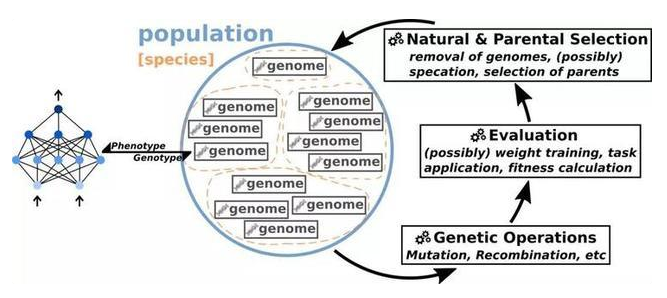
\includegraphics[width=0.85\textwidth]{GenerationElvovlilng2020020401.png}
\caption{典型的代际神经进化过程图解}
\label{GenerationElvovlilng2020020401}
\end{figure}
\end{remark}
%%%%%%%%%%%%%%%%%%%%%%%%%%%%%%%%%%%%
\begin{remark}
神经进化过程也是一个“黑盒”, 虽然它自己的进化过程需要参数, 但却不为生成的神经网络规定任何特定超参数, 而是根据实际问题的解决设计神经网络. 这便为神经网络的权重、超参数等的选择提供了范围, 此范围也称为搜索空间. 虽然“黑盒”性提供了非常广泛的搜索空间, 但是为了提高遍历搜索空间的速度, 明智的做法是限制搜索空间的粒度. 通过限制基因组编码的复杂性, 将基因组映射到搜索空间的粒度的能力也被称为遗传编码. 综上所述, 为了使搜索空间具有适当的粒度, 根据实际问题的要求, 设计遗传编码和相应的神经进化算法非常重要. 先来回顾一下遗传编码的概念.

有效的神经网络是能够进行有效的变异和重组人工神经网络的前提. 拥有强大表示能力的神经网络不用分析高度复杂的数据结构就能够快速的处理紧凑的遗传密码(compact genetic codes).
换句话说, 神经进化算法只在遗传编码上操作, 而不是在机器学习框架中复杂的数据结构上操作. 当然, 基因编码允许这两种表示之间存在映射关系. 基因组的这些有效的遗传表示被称为基因型(genotypes), 而相应映射的神经网络被称为显型(phenotypes), 这些术语来自遗传进化学. 这里将所有显型都限制为神经网络.

基因编码一般可分为两个子类:直接编码和间接编码. 虽然还有第三类发展性编码, 但这种编码我们先忽略不计, 毕竟这两年也没啥进展. 直接编码表示神经网络的各个方面, 它们在遗传表示中显式编码(如图\ref{IndirectGencode2020020401}所示). 直接编码直接在基因型中编码每个连接及其相应的权重, 但通过排除神经网络中的偏差和激活函数的可能性来限制搜索空间.
这种直接编码可以表示任意的前馈和递归拓扑, 也能够产生最优的拓扑. 但“拓扑”太灵活的话, 粒度的搜索空间就会变得非常庞大. 因此需要设计良好的神经进化算法才能快速遍历该搜索空间.
%%%%%%%%%%%%%%%%%%%%%%%%%%%%%%%%%%%%
\begin{figure}[H]
\centering
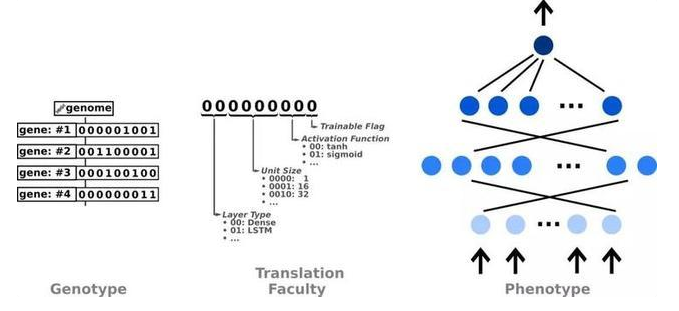
\includegraphics[width=0.75\textwidth]{IndirectGencode2020020401.png}
\caption{间接遗传编码}
\label{IndirectGencode2020020401}
\end{figure}

间接编码的功能是规定那些无法直接“翻译”成人工神经网络的自定义编码. 也就是说为了将基因型映射到神经网络, 需要一个由间接编码规定单独的“翻译”能力. 如果间接编码设计得当, 那么即使神经网络非常复杂, 也可以通过搜索空间实现有意义且快速的遍历.
虽然可以从直接编码快速创建人工神经网络, 但是缺少间接编码的翻译能力却会减慢处理速度, 并且可能导致“粗粒度”. 所以在决定使用哪种编码之前, 必须考虑两种编码的优缺点.
但是两种遗传编码都证明了遗传编码如何确定搜索空间的大小, 例如. 例如通过控制激活函数或某些层类型确定搜索空间.
\end{remark}

%%%%%%%%%%%%%%%%%%%%%%%%%%%%%%%%%%%%
\begin{remark}
有种遍历搜索空间的方法被称为繁殖的过程, 这种方法与神经进化所使用的遗传编码密切相关. 通常通过突变或重组基因组来创造新的基因组, 新的基因组也继承了旧的基因组. 突变让后代基因组探索人工神经网络新的结构、权重和超参数. 重组基因组本质上是将两个基因组及其独特的特征合并.
突变与遗传编码紧密相关, 因为神经网络的参数只能突变到以遗传编码表示的程度. 因此, 为神经进化算法定义突变有以下三种情况.

1) 遗传编码的哪一部分会发生突变?是拓扑变化、权重增减、还是超参数调节?

2) 基因组中选定的部分会发生多大程度的突变?
%%%%%%%%%%%%%%%%%%%%%%%%%%%%%
\begin{example}
  神经进化算法可以对低适应度基因组使用较大的突变, 对高性能基因组使用微小的突变.
\end{example}

3) 突变采用何种方式. 是定向还是随机?
%%%%%%%%%%%%%%%%%%%%%%%%%%%%%%%%%%%%
\begin{figure}[H]
\centering
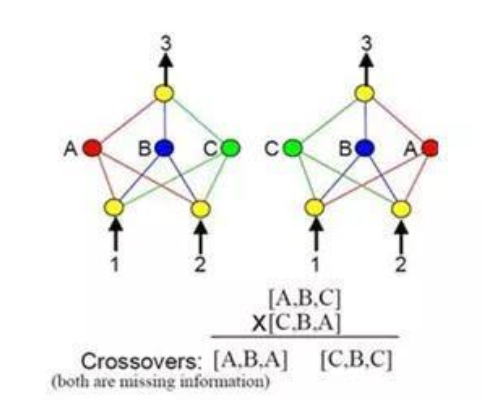
\includegraphics[width=0.65\textwidth]{Crossovers2020020402.png}
\caption{竞合公约问题图解}
\label{Crossovers2020020402}
\end{figure}

重组并不会突变基因组, 拥有创新可以通过将两个亲本基因组及其独特特征结合, 并产生“新颖”的后代基因组. 如果重组方法设计得当, 并且可以无损地融合两个亲本基因组的有益特征, 将其在整个群体中传播, 提高所有现有基因组的适用性.
设计重组方法的核心在于“无损融合”, 即不丢失任何基因特性的情况下融合.
%%%%%%%%%%%%%%%%%%%%%%%%%%%%%
\begin{example}
  在神经进化算法之前, NEAT算法(通过增强拓扑的进化神经网络, Evolving NN through Augmenting Topologies)利用直接编码在进行修改网络的拓扑结构, 包括新增节点和删除节点等操作时会产生交叉损失.
\end{example}

如图\ref{Crossovers2020020402}竞合公约问题( competing-conventions problem)所示. 随后, NEAT算法提出了一种“历史标记”的方法, 该方法为每个突变提供了唯一的标识符, 从而最终实现了基因组的无损重组, 使其为神经进化算法提供了基准.
\end{remark}

在总体优化循环中, 基于问题评估基因组似乎是最简单的. 但这一步骤确是非常重要, 不仅是能够指出潜在的改进和进步. 评估方法从根本上说是一个过程, 即将基因组映射到由其遗传编码规定的神经网络, 并将其应用于问题环境, 然后根据神经网络的表现计算适应值. 一些神经进化算法的评估过程还包括将神经网络加权训练的附加步骤, 虽然这种方法非常明智, 但只有当实际环境能够清晰反映基本信息才有用. 在整个评估过程中, 尽管确定适应度的方式完全取决于实际问题的具体情况, 但可以进行合理的修改. 例如在图像识别中可以设置为准确度, 游戏中可以设置为点数. 在确定适应度计算时, 新颖性搜索也是一个需要考虑的重要概念. 因为这个概念涉及用新的方法奖励基因组, 能够使其具有更高的适应值. 例如, 在实际的电子游戏环境中的智能体如果进入一个未知的区域会获得体能提升, 尽管总体上获得的分数较少, 但也能促进了基因库的创新, 从而促进更有希望的进化.
%%%%%%%%%%%%%%%%%%%%%%%%%%%%%%%%%%%%%%
\section{PSO}

%%%%%%%%%%%%%%%%%%%%%%%%%%%%%%%%%%%%%%
\section{QBFA}
%%%%%%%%%%%%%%%%%%%%%%%%%%%%%%%%%%%%%%
\section{其它算法*}
%%%%%%%%%%%%%%%%%%%%%%%%%%%%%
\subsection{鱼群算法}
%%%%%%%%%%%%%%%%%%%%%%%%%%%%%
\subsection{鸟群算法}
%%%%%%%%%%%%%%%%%%%%%%%%%%%%%
\subsection{象群算法}
%%%%%%%%%%%%%%%%%%%%%%%%%%%%%
\subsection{蚁群算法}
%%%%%%%%%%%%%%%%%%%%%%%%%%%%%
\subsection{狼群算法}
%%%%%%%%%%%%%%%%%%%%%%%%%%%%%
\subsection{蝙蝠算法}
%%%%%%%%%%%%%%%%%%%%%%%%%%%%%
\subsection{随机森林}
%%%%%%%%%%%%%%%%%%%%%%%%%%%%%%
\begin{figure}[H]
\begin{center}
\tikzset{marrow/.style={midway,red,sloped,fill, minimum height=3cm, single arrow, single arrow
    head extend=.5cm, single arrow head indent=.25cm,xscale=0.15,yscale=0.15,
    allow upside down}}
\scalebox{.5}{
\begin{forest}
for tree={l sep=3em, s sep=3em, anchor=center, inner sep=0.7em, fill=blue!50,
circle, font=\Large\sffamily,where level=1{no edge}{}}
  [Training Data, draw, rectangle, rounded corners, orange, text=white,alias=TD
    [,red!70,alias=a1[[,alias=a2][]][,red!70,edge label={node[above=1ex,marrow]{}}[[][]][,red!70,edge label={node[above=1ex,marrow]{}}[,red!70,edge label={node[below=1ex,marrow]{}}][,alias=a3]]]]
    [,red!70,alias=b1[,red!70,edge label={node[below=1ex,marrow]{}}[[,alias=b2][]][,red!70,edge label={node[above=1ex,marrow]{}}]][[][[][,alias=b3]]]]
    [~$\cdots$~,scale=4,no edge,fill=none,yshift=-1em]
    [,red!70,alias=c1[[,alias=c2][]][,red!70,edge label={node[above=1ex,marrow]{}}[,red!70,edge label={node[above=1ex,marrow]{}}[,alias=c3][,red!70,edge label={node[above=1ex,marrow]{}}]][,alias=c4]]]
  ]
\node[draw,fit=(a1)(a2)(a3)](f1){};
\node[draw,fit=(b1)(b2)(b3)](f2){};
\node[draw,fit=(c1)(c2)(c3)(c4)](f3){};
\path (f1.south west)--(f3.south east) node[midway,below=4em] (David) {mean};
\node[below=2em of David] (pred){prediction};
\foreach \X in {1,2,3}{\draw[-stealth] (TD) -- (f\X.north);
\draw[-stealth] (f\X.south) -- (David);}
\draw[-stealth] (David) -- (pred);
\end{forest}
}
\caption{语义网络的基本网元}
\label{AIRForestfig105}
\end{center}
\end{figure}
%%%%%%%%%%%%%%%%%%%%%%%%%%%%%
\subsection{ADP聚类算法}
\href{https://www.sciencedirect.com/science/article/pii/S0020025518303967}{A method for autonomous data partitioning}, 2018.8 \cite{GuAngelov2018-5667}

\href{https://github.com/Gu-X/Autonomous-Data-Partitioning-Algorithm}{ADP python}
%%%%%%%%%%%%%%%%%%%%%%%%%%%%%%%%%%%%%%%%%%%%%%%%%%%%%%%%%%%%%%%%%%%%%%%%%%%%%%%%
\begin{sidewaystable}[!ht]
\caption{Training and testing error on Auto-Mpg, Bank, Diabetes and Triazines.}
\begin{center}
 \begin{tabular}{lp{10cm}lcccccccc}
\toprule
%\multirow{2}{*}{Data set}&\multirow{2}{*}{Algorithm}&\multicolumn{2}{c}{Training (RMSE)}&\multicolumn{2}{c}{Testing (RMSE)}\\
%\cline{3-4}\cline{5-6}
 &  &  Web Link  \\
\toprule
Codes &ADP Algorithm &\small{\url{http://empiricaldataanalytics.org/downloads.html}}\\
&Pre-trained VGG-VD-16 convolutional neural network [46]&\small{\url{http://www.vlfeat.org/matconvnet/pretrained/}}\\
Datasets &PIMA [47] &\small{\url{https://archive.ics.uci.edu/ml/datasets/pima+indians+diabetes}}\\
&Banknote Authentication [37] &\small{\url{https://archive.ics.uci.edu/ml/datasets/banknote+authentication}}\\
&S1 [23] &\small{\url{http://cs.joensuu.fi/sipu/datasets/}}\\
&S2 [23] &\small{\url{http://cs.joensuu.fi/sipu/datasets/}}\\
&Cardiotocography [9] &\small{\url{https://archive.ics.uci.edu/ml/datasets/cardiotocography}}\\
&Pen-Based Handwritten Digits Recognition [2] &\small{\url{https://archive.ics.uci.edu/ml/datasets/Pen-Based+Recognition+of+
Handwritten+Digits}}\\
&Steel Plates Faults [14] &\small{\url{http://archive.ics.uci.edu/ml/datasets/steel+plates+faults}}\\
&Multiple Features [30] &\small{\url{https://archive.ics.uci.edu/ml/datasets/Multiple+Features}}\\
&Occupancy Detection [16] &\small{\url{https://archive.ics.uci.edu/ml/datasets/Occupancy+Detection+}}\\
&MAGIC Gamma Telescope [13] &\small{\url{https://archive.ics.uci.edu/ml/datasets/magic+gamma+telescope}}\\
&Letter Recognition [24] &\small{\url{https://archive.ics.uci.edu/ml/datasets/letter+recognition}}\\
&Singapore [26] &\small{\url{http://icn.bjtu.edu.cn/Visint/resources/Scenesig.aspx}}\\
&Caltech 101 [22] &\small{\url{http://www.vision.caltech.edu/Image_Datasets/Caltech101/}}\\
&MNIST [35] &\small{\url{http://yann.lecun.com/exdb/mnist/}}\\
\bottomrule
\end{tabular}
\end{center}
\label{TT2-ELM170610:Sec5-3-1}
\end{sidewaystable}
%%%%%%%%%%%%%%%%%%%%%%%%%%%%%%%
\href{https://ww2.mathworks.cn/matlabcentral/fileexchange/67463-autonomous-data-partitioning-algorithm?s_tid=prof_contriblnk}{ADP}

The package contains:

1. The recently introduced autonomous data partitioning algorithm;

2. A demo for offline data partitioning;

3. A demo for online data partitioning;

4. A demo for creating a hybrid between the offline and online versions

Reference: X. Gu, P. Angelov and J. Principe, “A Method for Autonomous Data Partitioning,” Information Sciences, 2018, DOI:10.1016/j.ins.2018.05.030.

For any queries about the codes, please contact Prof. Plamen P. Angelov (p.angelov@lancaster.ac.uk) and Mr. Xiaowei Gu (x.gu3@lancaster.ac.uk)

The proposed ADP algorithm has an offline version and an evolving version. Its offline version is based on the ranks of the data samples in terms of their densities and mutual distances instead of the commonly used means and variances. Ranks are very important but other approaches avoid them because they are nonlinear and discrete operators. Therefore,
the offline version is more stable and effective in partitioning static datasets. The evolving version is also generic and fully
data-driven. It can continue the offline partitioning process with the newly arrived data, but can also start without initial
conditions.

Lifting these assumptions is possible with information theoretic \cite{JenssenErdogmus2007-5673} and spectral clustering \cite{vonLuxburg2007-5674}, but at the expense of much higher computational cost.

The proposed ADP approach is proposed within the recently introduced Empirical Data Analysis (EDA)\index{Empirical Data Analysis} framework \cite{Angelov2014Outside,Angelov2016-7844219,Angelov2017Empirical}.
EDA resembles statistical learning in its nature but is free from the range of assumptions made in traditional probability theory and statistical learning approaches \cite{Angelov2014Outside,Angelov2016-7844219,Angelov2017Empirical}. EDA measures play an instrumental role in the proposed ADP approach for extracting the ensemble properties from the observed data (see Fig. 1(b)), and frees the ADP algorithm from the requirement to make prior assumptions on the data generation model and user- and problem-specific parameters (see Fig. 1(a)). Most importantly, they guarantee objectiveness of the partitioning results.

Firstly, we define the data set/stream in the Euclidean data space $\mathbb R^N$ as $\{\bm x\}_K = \{\bm x_1, \bm x_2, \cdots, \bm x_K\}$, $\bm x_k =[x_{k, 1}, x_{k, 2}, \cdots, x_{k, N}]^T \in \mathbb R^N$, where $k = 1, 2, \cdots, K$ is an order index. We, further, consider that some data samples within the data set/stream can have the same value, i.e. $\exists \bm x_k = \bm x_j, k\neq j$. The set of sorted unique data samples is denoted as $\{\bm u\}_{L_K} =\{\bm u_1, \bm u_2, \cdots, \bm u_{L_K}\},\bm u_j = [u_{j,1}, u_{j,2}, \cdots, u_{j,N}]^T ( j = 1, 2, \cdots, L_K), \{\bm u\}_{L_K} \subseteq \{\bm x\}_K , L_K \leq K$ with the corresponding occurrence frequencies
$\{f\}_{L_K} = \{ f_1, f_2, \cdots, f_{L_K}\},\sum\limits^{L_K}_{k=1} f_k = 1$.

In this paper, we use the natural metric of the space of samples (i.e. Euclidean distance) for clarity, however, various types of distances within the data space, $\mathbb R^N$ can be considered as well. In the remainder of this paper, all the derivations are conducted at the $K$th time instance except when specifically mentioned.

In this section, we will summarize the nonparametric EDA measures that we use in ADP:

I) local density, $D$ \cite{Angelov2016-7844219,Angelov2017Empirical};

II) global density, $D^G$ \cite{Angelov2016-7844219,Angelov2017Empirical};

and their recursive implementations to make the paper self-contained.


3.1. Local density

Local density \cite{Angelov2016-7844219} is a measure within EDA framework identifying the main local mode of the data distribution and is derived empirically from all the observed data samples in a parameter-free way. The local density, $D$ of the data sample $\bm x_k$ is expressed as follows $(k = 1, 2, \cdots, K; L_K > 1)$ \cite{Angelov2016-7844219,Angelov2017Empirical}:
\begin{align}\label{EDAlocaldensity18072401}
    D_K(\bm x_k) =\frac{\sum^K_{j=1}\sum^K_{l=1} d^2(\bm x_j,\bm  x_l)} {2K \sum^K_{l=1} d^2(\bm x_k,\bm  x_l)}
\end{align}
where $d(\bm x_k, \bm x_l)$ is the distance between data samples $\bm x_k$ and $\bm x_l$; the coefficient 2 is used in the denominator for normalization (because each distance is counted twice in the numerator).

For the case of Euclidean distance, the calculation of $\sum^K_{l=1} d^2(\bm x_k,\bm  x_l)=\sum^K_{l=1}\|\bm x_k-\bm  x_l\|^2$ and $\sum^K_{j=1}\sum^K_{l=1} d^2(\bm x_j,\bm  x_l)=\sum^K_{j=1}\sum^K_{l=1}\|\bm x_j-\bm  x_l\|^2 $ can be simplified by using the mean of $\{\bm x\}_K$, $\bm \mu_K$ and the average scalar product, $X_K$ as \cite{Angelov2016-7844219,Angelov2017Empirical}:
\begin{align}
  &\sum^K_{l=1}\|\bm x_k-\bm  x_l\|^2=K(\|\bm x_K-\bm \mu_K\|^2+X_K-\|\bm \mu_K\|^2)\label{EDAlocaldensity18072402}\\
  &\sum^K_{j=1}\sum^K_{l=1}\|\bm x_j-\bm  x_l\|^2 =2K^2(X_K-\|\bm \mu_K\|^2)\label{EDAlocaldensity18072403}
\end{align}
$\bm \mu_K$ and $X_K$ can be updated recursively as \cite{Angelov2012Autonomous}:
\begin{align}
  &\bm \mu_k=\frac {k-1} k \bm \mu_{k-1}+\frac {1} k \bm  x_k, \bm \mu_1=\bm x_1, k=1,2,\cdots, K\label{EDAlocaldensity18072404}\\
  &X_k=\frac {k-1} k X_{k-1}+\frac {1} k \|\bm x_k\|^2, X_1=\|\bm  x_1\|^2, k=1,2,\cdots, K\label{EDAlocaldensity18072405}
\end{align}
The recursive calculation of $\bm \mu_K$ and $X_K$ allows for “one pass” calculation, thus, ensures computation-efficiency because only the key aggregated/summarized information has to be kept in memory.

Combining \eqref{EDAlocaldensity18072401}-\eqref{EDAlocaldensity18072405}, we can re-formulate the local density, $D$ in a recursive form:
\begin{align}\label{EDAlocaldensity18072406}
 D_K(\bm x_k) =\frac 1 {1 + \frac{\|\bm x_k-\bm\mu_K\|^2}{X_K-\|\bm \mu_K\|^2}}
\end{align}
From \eqref{EDAlocaldensity18072406} we can see that when the Euclidean distance is used, the local density, $D$ behaves as a \textbf{Cauchy function}\index{Cauchy function}, while there is \textbf{no prior assumption about the type of the distribution involved}. Note that $0 < D_K(\bm x_k) \leq 1$ and the closer $\bm x_k$ is to the main local mode, the higher the value of $D_K(\bm x_k)$ is.

3.2. Global density

The global density, $D^G$ estimated at the unique data sample $\bm u_k$ is a weighted sum of its local density by the corresponding occurrence, $f_k (k = 1, 2, \cdots, L_K;L_K > 1)$, expressed as follows \cite{Angelov2016-7844219,Angelov2017Empirical}:
\begin{align}\label{EDAlocaldensity18072407}
 D^G_K(\bm u_k) = \frac {f_k} {\sum_{j=1}^{L_K} f_j} D_K(\bm u_k) =  \frac {f_k}{1 + \frac{\|\bm u_k-\bm\mu_K\|^2}{X_K-\|\bm \mu_K\|^2}}
\end{align}
It is clear that it behaves locally as a Cauchy function, but has multiple local modes/peaks which depend on $f_k$ (if $L_K = K$, global density reduces to the local density but with a smaller amplitude). The largest of the peaks is called the global peak. The global density can directly disclose the data pattern without any further pre-processing. This property can be very useful in real cases where the units of measurement are fixed and data samples measured at different indices are likely to share the same values. The reason we do not stop with $D^G$ but move further with partitioning is that although it is fully automatic and objective, $D^G$ often reveals too many local peaks.

4. The autonomous data partitioning algorithm

In this section, we will describe the proposed ADP algorithm for further refining the local modes of the data set/stream. The local modes are defined as the local maxima of the global data density and are constructed directly from samples. These local modes play a key role in partitioning the data space into shape-free data clouds \cite{Angelov2012Autonomous,Angelov2014Outside} by aggregating data samples around them and forming naturally a Voronoi tessellation \cite{OkabeBoots2000-5677}. We will present two independent algorithms for the two versions, i) offline and ii) evolving.

4.1. Offline ADP algorithm

The offline ADP algorithm works with the global density, $D^G$ of the observed data samples. It is based on the ranks of the data samples in terms of their global densities and mutual distributions. Its main procedure is described as follows:

Stage 1: \textbf{Rank order the samples with regards to the distance to the global mode}

We start by organizing the unique data samples $\{\bm u\}_K$ into an indexing list, denoted by $\{\bm u^*\}_K$ based on their mutual distances and values of the global density, $D^G$.
Firstly, the global densities of the unique data samples, $D^G_K(\bm u_i) (i = 1, 2, \cdots, L_K)$ are calculated using \eqref{EDAlocaldensity18072407}. The unique data sample with the highest global density is then selected as the first element of the indexing list $\{\bm u^*\}_{L_K}$:
\begin{align}\label{EDAlocaldensity18072408}
 \bm u^{*1} = {\arg \max}_{j=1,2,\cdots,L_K} \left(D^G_K(\bm u_j)\right)
\end{align}
We set $\bm u^{*1}$ as the first reference point: $\bm u^{*r} \leftarrow \bm u^{*1}$ and remove $ \bm u^{*1}$ from $\{\bm u\}_{L_K}$. Then, by selecting out the unique data
sample which is nearest to $\bm u^{*r}$, the second element of $\{u^*\}_{L_K}$ denoted by $u^{*2}$ is identified and it is set as the new reference point $\bm u^{*r} \leftarrow \bm u^{*2}$ and, is also removed from $\{\bm u\}_{L_K}$. The process is repeated until $\{\bm u\}_{L_K}$ becomes empty, and the rank ordered list $\{\bm u^*\}_{L_K}$ is finally derived. Based on this list, we can rank the global density of the unique data samples as:
\begin{align}\label{EDAlocaldensity18072409}
 \left\{D^G_K(\bm u^*)\right\} =\{D^G_K(\bm u^{*1}),D^G_K(\bm u^{*2}),\cdots, D^G_K(\bm u^{*L_K}) )\} .
\end{align}
An example using the wine dataset \cite{AeberhardWinedata1992} is shown in Fig. 2. Fig. 2(a) shows the global density of the wine dataset, Fig. \ref{RankedDGlocalMaxima0726}
shows the ranked global density.
%%%%%%%%%%%%%%%%%%%%%%%%%%%%%%%%2018-7-26
\begin{figure}[H]
\centering
  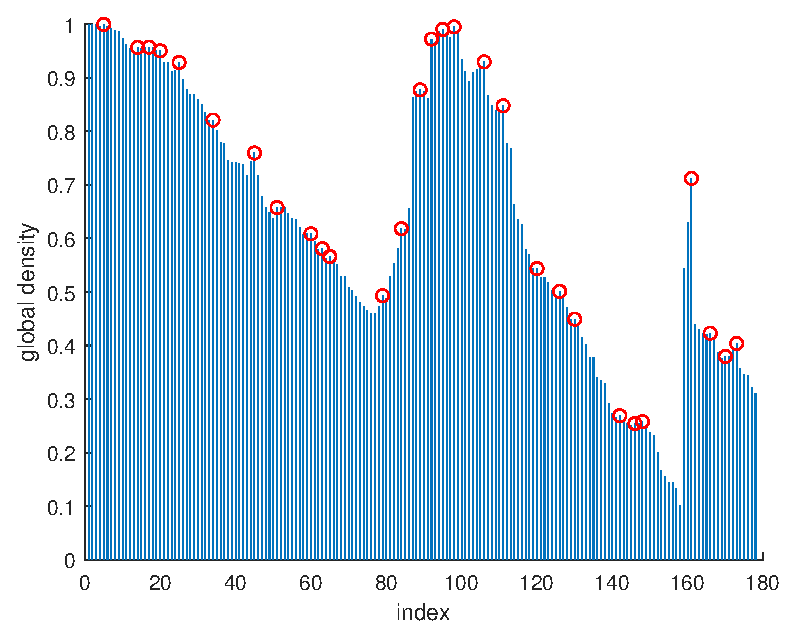
\includegraphics[width=.45\textwidth]{RankedDGlocalMaxima.eps}
  \caption{The ranked $D^G$ and the identified local maxima.}
  \label{RankedDGlocalMaxima0726}
\end{figure}
%%%%%%%%%%%%%%%%%%%%%%%%%%%%%%%%
%%%%%%%%%%%%%%%%%%%%%%%%%%%%%%%%
\begin{figure}[H]
\centering
  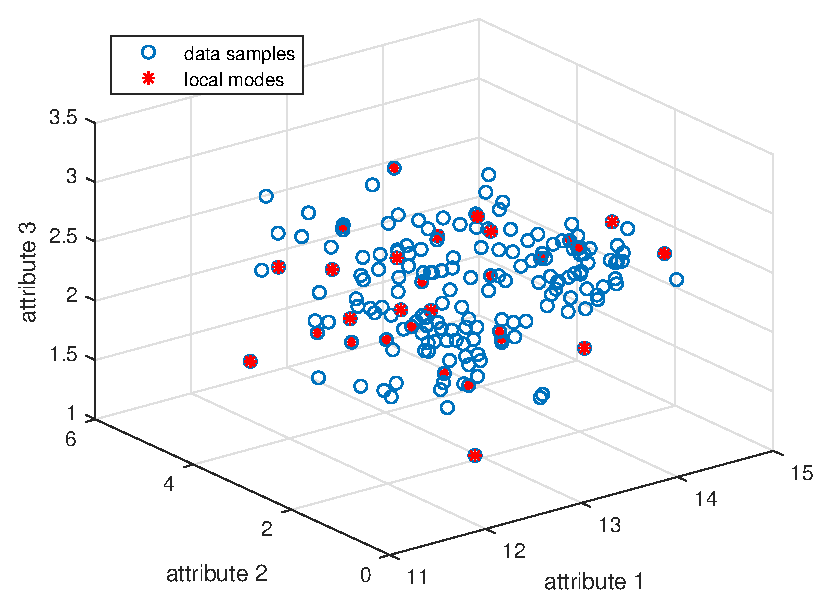
\includegraphics[width=.45\textwidth]{DGlocalMaxima3D.eps}
  \caption{The location of local maxima in the data space.}
  \label{DGlocalMaxima3D0726}
\end{figure}
%%%%%%%%%%%%%%%%%%%%%%%%%%%%%%%%
Stage 2: \textbf{Detecting local maxima (local modes)}

Based on the list $\{\bm u^*\}_{L_K}$ and the ranked global density $\{D^G_K(\bm u^*)\}$, we can identify all the data samples with the local maxima of $D^G$ directly as follows:
\begin{align}\label{EDAlocaldensity18072410}
\textup{IF}\, \textup{sgn} D^G_K(\bm u^{*j})- &D^G_K(\bm u^{*j+1}) = 1\,  \textup{AND}\, \textup{sgn} D^G_K(\bm u^{*j-1}) - D^G_K(\bm u^{*j}) =-1 \notag\\
                                             &\textup{THEN}\, \bm u^{*j}\,\textup{is a local maximum of}\, D^G
\end{align}
where
\begin{align*}
\textup{sgn}(x)
\left\{
\begin{array}{ll}
1,& x > 0\\
0,& x = 0\\
−1,& x < 0
\end{array}
\right.
\end{align*}
is the sign function; we denote the collection of data samples with the local maxima of $D^G$ as $\{u^{**}\}_{L_K^*}= {u^{** j}|j = 1, 2, \cdots, L_K^*} (L_K^* < L_K)$. The local maxima (peaks) identified from the wine dataset \cite{AeberhardWinedata1992} are marked by red circles in Fig. 2(b). The locations of the local maxima in the data space are depicted in Fig. \ref{DGlocalMaxima3D0726}.

Stage 3: \textbf{Forming data clouds}

The local peaks identified from the indexing list, namely, $\{u^{**}\}L_K^*$, are then used to attract the data samples $\{\bm x\}_K$ that are closer to them using a min operator:
\begin{align}\label{EDAlocaldensity18072411}
\textup{winning cloud} = {\arg \min}_{ j=1,2,\cdots,L_ K^*} (\|\bm x_i-u^{**j}\|)\, i=1,2,\cdots, K; L_K^*>1
\end{align}

By assigning all the data samples to the nearest local maxima, a number of Voronoi tessellations \cite{OkabeBoots2000-5677} are naturally formed and data clouds are built around the local maxima \cite{Angelov2012Autonomous,Angelov2014Outside}. More importantly, the process is free from any threshold.

After the data clouds are formed, the actual centre (mean) $\mu_j$ and the standard deviation $\sigma_j ( j = 1, 2, \cdots, L_K^*)$ per data cloud and the support, $S^j$, namely, the number of data samples within the data cloud can be calculated easily. Note that, all this procedure is post factum, i.e. it is determined bottom up from the data without a prior assumption, except the selection of the metric.

Stage 4: \textbf{Filtering local modes}

The data clouds formed in the previous stage may contain some less representative ones; therefore, in this stage, we filter the initial Voronoi tessellations and combine them into larger, more meaningful data clouds.
The global densities at the data clouds centres $\{\bm\mu\}_{L_K^*}$ are firstly calculated as follows $( j = 1, 2, \cdots, L_K^*)$:
\begin{align}\label{EDAlocaldensity18072412}
 D^G_K(\bm\mu^j ) = \frac{S^j}{1 +\frac{\|\bm\mu^j-\bm\mu_K\|^2}{X_K-\|\bm \mu_K\|^2} }
\end{align}
where $S^j$ is the support of the data cloud.

In order to identify the centres with the local maxima of the global density, we introduce the following three objectively derived quantifiers of the data pattern:
\begin{align}
&\eta_K^c = 2\sum^{L^*_K-1}_{ p=1}\sum^{L^*_K}_{q=p+1} \|\bm \mu^p - \bm \mu^q\|  /L^*_K({L^*_K-1})\label{EDAlocaldensity18072413}\\
&\gamma_K^c =\frac{\sum\limits_{\bm x\neq \bm y, \|\bm x-\bm y\|\leq \eta_K^c,\bm x,\bm y\in \{\bm\mu\}_{L_K^*}}\|\bm x-\bm y\|}{M_\eta}\label{EDAlocaldensity18072414}\\
&\lambda_K^c =\frac{\sum\limits_{\bm x\neq \bm y, \|\bm x-\bm y\|\leq \gamma_K^c,\bm x,\bm y\in \{\bm\mu\}_{L_K^*}}\|\bm x-\bm y\|}{M_\gamma}\label{EDAlocaldensity18072415}
\end{align}
$\eta_K^c$ is the average Euclidean distance between any pair of existing local modes. $\gamma_K^c$ is the average Euclidean distance between any pair of existing local modes within a distance less than $\eta_K^c$, and $M_\eta$ in \eqref{EDAlocaldensity18072413} is the number of such local mode pairs. $\lambda_K^c$ is the average Euclidean distance between any pair of existing local modes within a distance less than $\gamma_K^c$, $M_\gamma$ in \eqref{EDAlocaldensity18072415} is the number of such local mode pairs.

Note that $\eta_K^c, \gamma_K^c$ and $\lambda_K^c$ are not problem- specific and are parameter-free. The relationship between $\eta_K^c, \gamma_K^c$ and $\lambda_K^c$ is depicted in Fig. 3 using the wine dataset \cite{AeberhardWinedata1992} again, where one can see that $\lambda_K^c$ is a smaller value compared with $\eta_K^c$ and $\gamma_K^c$ which are obtained as the average distance of two very close data cloud centres.
The quantifier $\lambda_K^c$ can be viewed as the estimation of the distances between the strongly connected data clouds condensing the local information from the whole dataset. Moreover, instead of relying on a fixed threshold, which may frequently fail, $\eta_K^c, \gamma_K^c$ and $\lambda_K^c$ are derived from the dataset objectively and conforming with the concept of a mode. Experience has shown that they provide meaningful tessellations, regardless of the distribution of the data.

Each centre $\bm\mu^j( j = 1, 2, \cdots, L_K^*)$ is compared with the centres of neighbouring data clouds in terms of the global density:
\begin{align}\label{EDAlocaldensity18072416}
\textup{IF}\,  D^G_K(\bm u^{j})=\max \left\{ \left\{D^G_K(\bm \mu)\right\}_n^j,D^G_K(\bm \mu^j)\right\}\, \textup{THEN}\, \bm u^{j}\,\textup{is a local maximum}
\end{align}
where $\left\{ D^G(\bm u^{*j}) \right\}_n^j$ is the collection of global densities of the neighbouring centres, which satisfy the following condition:
\begin{align}\label{EDAlocaldensity18072417}
\textup{IF}\,  \left(\|\bm \mu^i-\bm \mu^j\|\leq \frac{\lambda_K^c}{2}\right)\, \textup{THEN}\, \bm u^{i}\,\textup{is neighbouring }\bm u^{j}
\end{align}
The criterion of neighbouring range is defined in this way because two centres with the distance smaller than $\gamma_K^c$ can be considered to be potentially relevant in the sense of spatial distance; $\lambda_K^c$ is the average distance between the centres of any two potentially relevant data clouds. Therefore, when the condition (16) is satisfied, both $\bm \mu^i$ and $\bm \mu^j$ are highly influencing each other and, the data samples within the two corresponding data clouds are strongly connected. Therefore, the two data clouds are considered as neighbours. This criterion also guarantees that only small-size (less important) data clouds that
significantly overlap with large-size (more important) ones will be removed during the filtering operation.

After the filtering operation (stage 4), the data cloud centres with local maximum global densities denoted by
$\{\bm \mu^{*}\}_{L_K^{**}}={\bm \mu^{*j}| j = 1, 2, \cdots, L_K^{**} , L_K^{**} \leq L_K^{*}}$ are obtained. Then, $\{\bm \mu^*\}L_K^{**}$ are used as local modes for forming data clouds in stage 3 and are filtered in stage 4.

Stages 3 and 4 are repeated until all the distances between the existing local modes exceed $\frac{\lambda_K^c} 2$. Finally, we obtain the remaining centres with the local maxima of $D^G$, denoted by $\{\bm\mu^o\}$, and use them as the local modes to form data clouds
using \eqref{EDAlocaldensity18072410}.

After the data clouds are formed, the corresponding centres, standard deviations, supports, members and other parameters of the formed data clouds can be extracted post factum. The final partitioning result of the wine dataset \cite{AeberhardWinedata1992} is depicted in Fig. 4, where the dots in different colours stand for data samples from different data clouds, the black asterisks stand for
the centres of the data clouds.

4.2. Evolving ADP algorithm

The proposed evolving ADP algorithm works with the local density, D of the streaming data. This algorithm is able to start “from scratch”, i.e. with a single sample. In addition, a hybrid between the evolving and the offline versions is also possible.

The main procedure of the evolving algorithm is as follows.

Stage 1: Initialization

We select the first data sample within the data stream as the first local mode. The proposed algorithm then starts to self-evolve its structure and update the parameters based on the arriving data samples.

Stage 2: System structure and meta-parameters update

For each newly arrived data sample at the current time instance $k \leftarrow k + 1$, denoted as $\bm x_k$, the global meta-parameters $\bm \mu_k$ and $X_k$ are updated with $\bm x_k$ firstly using \eqref{EDAlocaldensity18072404} and \eqref{EDAlocaldensity18072405}. The local density at $\bm x_k$ and the centres of all the existing data clouds, $D_k(\bm x_k)$ and $D_k(\bm \mu^i _k) (i = 1, 2, \cdots ,C_k)$ are calculated using \eqref{EDAlocaldensity18072406}; here, we use $C_k$ as the number of existing local modes at the $k$th
time instance.

Then, the following condition \cite{Angelov2012Autonomous} is checked to decide whether $\bm x_k$ will form a new data cloud:
\begin{align}\label{EDAlocaldensity18072417}
  \textup{IF}\, D_k(\bm x_k) > &\max_{i=1}^{C_k } (D_k(\bm \mu^i _k))\, \textup{OR}\, D_k(\bm x_k) < \min_{i=1}^ {C_k} (D_k(\bm \mu^i _k))\notag\\
    &\textup{THEN}\, (\bm x_k\,  \textup{becomes a new f ocal point})
\end{align}
If the condition is met, a new data cloud is added with $\bm x_k$ as its local mode $(C_k \leftarrow C_k + 1,\mu_k^{C_k} \leftarrow x_k$ and $S_k^{C_k} \leftarrow 1)$.
Otherwise, the existing local mode closest to $\bm x_k$ is found, denoted as $\bm \mu^n_k$. Then, the following condition is checked before $\bm x_k$ is assigned to the data cloud formed around $\bm \mu^n_k$:
\begin{align}\label{EDAlocaldensity18072418}
  \textup{IF}\, \||\bm x_k - \bm\mu^n_k\| \leq \frac{\eta^k_c} 2, \textup{THEN}\, (\bm x_k\, \textup{is assigned to}\, \bm\mu^n_k)
\end{align}

However, it is not computationally efficient to calculate $\eta_k^c$ at each time when a new data sample arrives. Since the average distance between all the data samples $\eta_k^d$ is approximately equal to $\eta_k^c$, $\eta_k^c\approx \eta_k^d$, $\eta_k^c$ can be replaced as:
\begin{align}\label{EDAlocaldensity18072419}
  \eta_k^c\approx \eta_k^d=\sqrt{\frac{\sum_{i=1}^k\sum_{l=1}^k \|\bm x _i-\bm x _l\|^2 }{k^2}}=\sqrt{2(X_k-\|\bm\mu_k\|^2)}
\end{align}
If the condition \eqref{EDAlocaldensity18072418} is satisfied, then $\bm x_k$ is associated with the nearest existing local mode $\bm \mu^n_k$ and the meta-parameters of $\bm \mu^n_k$ are updated as follows:
\begin{align}
  &S^n_k \leftarrow S^n_k + 1 \label{EDAlocaldensity18072420}\\
  &\bm\mu^n_ k \leftarrow \frac{S^n_k  - 1}{S^n_k}\bm \mu^n_k + \frac 1 {S^n_k}\bm x_k\label{EDAlocaldensity18072421}
\end{align}
If the condition \eqref{EDAlocaldensity18072418} is not satisfied, then $\bm x_k$ starts a new data cloud: $(C_k \leftarrow C_k + 1,\mu_k^{C_k} \leftarrow \bm x_k$ and $S_k^{C_k} \leftarrow 1)$.
The local modes and supports of other data clouds that do not get the new data sample stay the same for the next processing cycle. After the update of the system structure and the meta-parameters, the algorithm is ready for the next data sample.

Stage 3: Forming data clouds

When there are no more data samples, the identified local modes (renamed as $\{\bm \mu^o\}$) are used to build data clouds using \eqref{EDAlocaldensity18072411}. The parameters of these data clouds can be extracted post factum.
The main procedure of the proposed ADP algorithm (evolving version) is presented in the following pseudo code.

In this subsection, a number of benchmark datasets are used in the performance evaluation as tabulated in Table 1. During the experiments, we assume that we do not have any prior knowledge about the benchmark datasets. The following well-known algorithms are used for comparison: \index{Clustering Algorithms}
\begin{enumerate}[label=\Roman*,align=left]
  \item MS: Mean-shift clustering algorithm 2002 \cite{DPComaniciu2002-5678};
  \item SUB: Subtractive clustering algorithm 1994 \cite{Chiu1994-5679};  subclust--Find cluster centers using subtractive clustering-matlab 2006a up
  \item DBS: DBScan clustering algorithm 1996 \cite{EsterKriegel1996-5680};

  \url{http://yarpiz.com/255/ypml110-dbscan-clustering}
  \item SOM: Self-organizing map algorithm 1997 \cite{Kohonen1997-5691};
  \item ELM: Evolving local means clustering algorithm 2012 \cite{RPDutta2012-5681};
  \item DP: Density peaks clustering algorithm 2014 Science \cite{RodriguezLaio2014-5691};
  \item NMM: Nonparametric mixture model based clustering algorithm 2006\cite{Blei2006-5683};
  \item NMI: Nonparametric mode identification based clustering algorithm 2007 \cite{LiRay2007-5690};
  \item CEDS: Clustering of evolving data streams algorithm 2017 \cite{HydeAngelov2017-5682}.
\end{enumerate}

Fully online clustering of evolving data streams into arbitrarily shaped clusters, 2017 \cite{HydeAngelov2017-5682} \index{Clusters-Arbitrarily Shaped }

In recent times there has been an increase in data availability in continuous data streams and clustering of this data has many advantages in data analysis. It is often the case that these data streams are not stationary, but evolve over time, and also that the clusters are not regular shapes but form arbitrary shapes in the data space. Previous techniques for clustering such data streams are either hybrid online / offline methods, windowed offline methods, or find only hyper-elliptical clusters. In this paper we present a fully online technique for clustering evolving data streams into arbitrary shaped clusters. It is a two stage technique that is accurate, robust to noise, computationally and memory efficient, with a low time penalty as the number of data dimensions increases. The first stage of the technique produces micro-clusters and the second stage combines these micro-clusters into macro-clusters. Dimensional stability and high speed is achieved through keeping the calculations both simple and minimal using hyper-spherical micro-clusters. By maintaining a graph structure, where the micro-clusters are the nodes and the edges are its pairs with intersecting micro-clusters, we minimise the calculations required for macro-cluster maintenance. The micro-clusters themselves are described in such a way that there is no calculation required for the core and shell regions and no separate definition of outer micro-clusters necessary. We demonstrate the ability of the proposed technique to join and separate macro-clusters as they evolve in a fully online manner. There are no other fully online techniques that the authors are aware of and so we compare the technique with popular online / offline hybrid alternatives for accuracy, purity and speed. The technique is then applied to real atmospheric science data streams and used to discover short term, long term and seasonal drift and their effects on anomaly detection. As well as having favourable computational characteristics, the technique can add analytic value over hyper-elliptical methods by characterising the cluster hyper-shape using Euclidean or fractal shape factors. Because the technique records macro-clusters as graphs, further analytic value accrues from characterising the order, degree, and completeness of the cluster-graphs as they evolve over time.


Rodriguez, Alex and Laio, Alessandro, \cite{RodriguezLaio2014-5691}, Clustering by fast search and find of density peaks, Science 2014 \index{Science}\index{Local Density Maxima}\index{Local Density Maxima}

Cluster analysis is used in many disciplines to group objects according to a defined measure of distance. Numerous algorithms exist, some based on the analysis of the local density of data points, and others on predefined probability distributions. Rodriguez and Laio devised a method in which the cluster centers are recognized as local density maxima that are far away from any points of higher density. The algorithm depends only on the relative densities rather than their absolute values. The authors tested the method on a series of data sets, and its performance compared favorably to that of established techniques. Cluster analysis is aimed at classifying elements into categories on the basis of their similarity. Its applications range from astronomy to bioinformatics, bibliometrics, and pattern recognition. We propose an approach based on the idea that cluster centers are characterized by a higher density than their neighbors and by a relatively large distance from points with higher densities. This idea forms the basis of a clustering procedure in which the number of clusters arises intuitively, outliers are automatically spotted and excluded from the analysis, and clusters are recognized regardless of their shape and of the dimensionality of the space in which they are embedded. We demonstrate the power of the algorithm on several test cases.

%%%%%%%%%%%%%%%%%%%%%%%%%%%%%%%%%%%%%%%%%%%%%%%%%%%%%%%%%%%%%%%%%%%%%%%%%%%%%%%%
\begin{table*}[!ht]
\caption{Details of the benchmark datasets for evaluation.}
\begin{center}
 \begin{tabular}{lp{8cm}lcccccccc}
\toprule
%\multirow{2}{*}{Data set}&\multirow{2}{*}{Algorithm}&\multicolumn{2}{c}{Training (RMSE)}&\multicolumn{2}{c}{Testing (RMSE)}\\
%\cline{3-4}\cline{5-6}
Abbreviation& Dataset& $N_A$b &$N_S$c &$N_C$d \\
\hline
PI& PIMA \cite{SmithEverhart1988-5692} &8& 768& 2\\
BA& Banknote Authentication \cite{LohwegHoffmann2013-5693}& 4 &1372 &2\\
S1& S1 \cite{FrantiVirmajoki2006-5694}& 2 &5000 &15\\
S2& S2 \cite{FrantiVirmajoki2006-5694}&2 &5000 &15\\
CA& Cardiotocography \cite{AyreseCamposBernardes2000-5695}& 22& 2126& 3\\
PB& Pen-Based Handwritten Digits Recognition \cite{AlimogluAlpaydin1996-5696}& 16 &10,992& 10\\
ST& Steel Plates Faults \cite{Buscema1998-5698}& 27 &1941 &7\\
MU& Multiple Features \cite{ARJain2000-5703} &649 &2000& 10\\
OD& Occupancy Detection \cite{CandanedoFeldheim2016-5699}a& 5 &20,560& 2\\
MA& MAGIC Gamma Telescope \cite{BockChilingarian2004-5701}& 10 &19,020& 2\\
LE& Letter Recognition \cite{FreySlate1991-5702} &16 &20,000 &26\\
\bottomrule
\end{tabular}
\end{center}
\label{TT2-ELM170610:Sec5-3-1}
\end{table*}
%%%%%%%%%%%%%%%%%%%%%%%%%%%%%%%
a The time stamps in the original dataset have been removed.
b Number of attributes.
c Number of samples.
d Number of classes.
%%%%%%%%%%%%%%%%%%%%%%%%%%%%%%%%%%%%%%
\section{模糊计算}
美国加州大学扎德(Zadeh)教授于1965年提出的模糊集合与模糊逻辑理论是模糊计算的数学基础. 它主要用来处理现实世界中因模糊而引起的不确定性. 目前, 模糊理论已经在推理、控制、决策等方面得到了非常广泛的应用. 本节主要讨论模糊理论的基础, 对于模糊推理将放到下一章讨论.

20世纪70年代中期, 中国开始引进模糊数学. 80年代在理论研究和应用研究方面都非常活跃并取得了大量研究成果, 主要代表人物有著名数学家汪培庄、张文修、蒲保明、刘应明、王国俊等教授. 1988年, 汪培庄教授及其指导的几名博士生研制成功一台模糊推理机——分立元件样机, 它的推理速度为1500万次/秒; 这表明中国在突破模糊信息处理难关方面迈出了重要的一步, 确实是一项了不起的研究成果. 2005年, 中国科学院院士刘应明教授((1940.10.8-2016.7.15), 福建福州人, 数学家, 中国科学院院士. 主要从事拓扑学与不确定性(主要是模糊性)数学处理等方面的教学与科学研究. 被誉为“中国的查德(模糊数学奠基人)")获国际模糊系统协会(IFSA)授予“Fuzzy Fellow”称号, 他是作为首位非发达国家学者获此殊荣的.
%%%%%%%%%%%%%%%%%%%%%%%%%%%%%%%%%%%%%%%%%%
\begin{figure}[H]
\centering
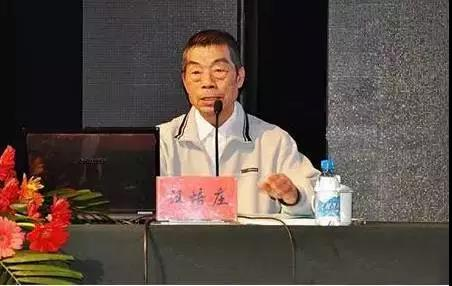
\includegraphics[width=0.46\textwidth]{WPZ20191218122443.jpg}
\caption{汪培庄教授}
\label{WPZ20191218122443}
\end{figure}
%%%%%%%%%%%%%%%%%%%%%%%%%%%%%%%%%%%%%%%%%%
\begin{figure}[H]
\centering
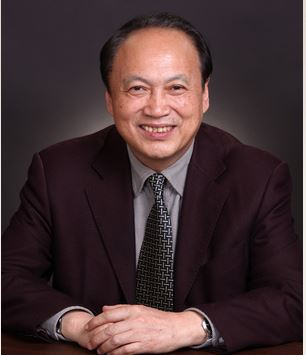
\includegraphics[width=0.46\textwidth]{Liuyingmingyuanshi.JPG}
\caption{刘应明院士}
\label{WPZ20191218122443}
\end{figure}
1983年国际模糊系统协会筹备会在法国马xi�举行, 参加会议的我国学者有, 刘应明(四川大学), 汪培庄(北师大), 王震源(河北大学), 邓聚龙(华中科大)和我共五人. 图为在会议组织委员会主席Sanchez家中合影.

%%%%%%%%%%%%%%%%%%%%%%%%%%%%%%%%%%%%%%%%%%
\begin{figure}[H]
\centering
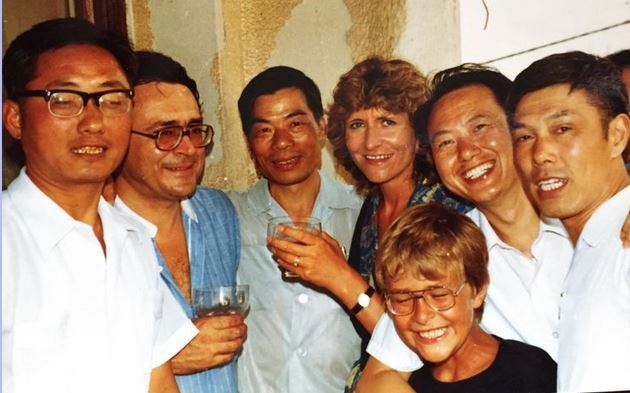
\includegraphics[width=0.46\textwidth]{IFSA1983.JPG}
\caption{1983年国际模糊系统协会筹备会在法国马xi举行, 参加会议的我国学者有, 刘应明(四川大学), 汪培庄(北师大), 王震源(河北大学), 邓聚㔫(华中科大)和张文修(西交大)}
\label{WPZ20191218122443}
\end{figure}
%%%%%%%%%%%%%%%%%%%%%%%%%%%%%%%%%%%%%%%%%%
中国著名学者周海中教授曾指出:“模糊数学的诞生,是科学技术发展的必然结果, 更是现代数学发展的必然产物. 但就现状而言,模糊数学的理论尚未成熟、体系还未形成, 对它也还存在不同看法和意见; 这些都有待日后完善和实践检验. ”
%%%%%%%%%%%%%%%%%%%%%%%%%%%%%%%%%%
\begin{mydef}{模糊集}{1}
设$U$是给定论域,   是把任意$u\in U$映射为$[0, 1]$上某个实值的函数, 即
\begin{align}
  U&\rightarrow [0, 1]\\
  u&\rightarrow \mu_F(u)
\end{align}
则称 $ \mu_F(x)$为定义在$U$上的一个隶属函数, 由   (对所有    )所构成的集合$F$称为$U$上的一个模糊集, 称为$u$对$F$的隶属度.
\end{mydef}

%%%%%%%%%%%%%%%%%%%%%%%%%%%%%%%%%%
\begin{remark}
\ding{172} 模糊集$F$完全是由隶属函数$\mu_{F}$来刻画的, 把$U$中的每一个元素$u$都映射为$[0, 1]$上的一个值$\mu_F(x)$ .

\ding{173} $\mu_F(u)$的值表示$u$隶属于$F$的程度, 其值越大, 表示$u$隶属于$F$的程度越高. 当$\mu_F(u)$仅取0和1时, 模糊集$F$便退化为一个普通集合.
\end{remark}
%%%%%%%%%%%%%%%%%%%%%%%%%%%%%%%%%%%%%%
\subsection{模糊集及其运算}
%%%%%%%%%%%%%%%%%%%%%%%%%%%%%%%
\begin{example}
  设论域$U=\{20, 30, 40, 50, 60\}$给出的是年龄, 请确定一个刻画模糊概念“年轻”的模糊集$F$.
\end{example}

解: 由于模糊集是用其隶属函数来刻画的, 因此需要先求出描述模糊概念“青年”的隶属函数. 假设对论域$U$中的元素, 其隶属函数值分别为:
\begin{align}
 \begin{array}{l}{\mu_{F}(20)=1, \mu_{F}(30)=0.8, \mu_{F}(40)=0.4} \\ {\mu_{F}(50)=0.1, \mu_{F}(60)=0}\end{array}
\end{align}
则可得到刻画模糊概念“年轻”的模糊集
\begin{align}
  F=\{ 1, 0.8, 0.4, 0.1, 0\}
\end{align}
说明其含义.

(1) 离散且为有限论域的表示方法

设论域 $U=\{u_1, u_ 2, \ldots, u_n\}$为离散论域, 则其模糊集可表示为:
\begin{align}
  F=\left\{\mu_{F}\left(u_{1}\right), \mu_{F}\left(u_{2}\right), \ldots, \mu_{F}\left(u_{n}\right)\right\}
\end{align}
为了能够表示出论域中的元素与其隶属度之间的对应关系, 扎德引入了一种模糊集的表示方式: 先为论域中的每个元素都标上其隶属度, 然后再用“+”号把它们连接起来, 即
\begin{align}
  F=\mu_{F}\left(u_{1}\right) / u_{1}+\mu_{F}\left(u_{2}\right) / u_{2}+\cdots+\mu_{F}\left(u_{n}\right) / u_{n}
\end{align}
也可写成
\begin{align}
  F=\sum_{i=1}^{n} \mu_{F}\left(u_{i}\right) / u
\end{align}
其中, $\mu_{F}\left(u_{i}\right)$为$u_i$对$F$的隶属度; “$\mu_{F}\left(u_{i}\right) |u_{i}$”不是相除关系, 只是一个记号; “+”也不是算术意义上的加, 只是一个连接符号.
\begin{align}
\begin{array}{ll}
F=\left\{\mu_{F}\left(u_{1}\right) / u_{1}, \mu_{F}\left(u_{2}\right) / u_{2}, \cdots, \mu_{F}\left(u_{n}\right) / u_{n}\right\} \\
F=\left\{\left(\mu_{F}\left(u_{1}\right), u_{1}\right),\left(\mu_{F}\left(u_{2}\right), u_{2}\right), \cdots,\left(\mu_{F}\left(u_{n}\right), u_{n}\right)\right\}
\end{array}
\end{align}
在这种表示方法中, 当某个$u_i$对$F$的隶属度=0时, 可省略不写.
\begin{example}
前面例5.15的模糊集$F$可表示为:
\begin{align}
  F=1 / 20+0.8 / 30+0.6 / 40+0.2 / 50
\end{align}
    有时, 模糊集也可写成如下两种形式:
\begin{align}
\begin{array}{l}
F=\left\{\mu_{F}\left(u_{1}\right) / u_{1}, \mu_{F}\left(u_{2}\right) / u_{2}, \cdots, \mu_{F}\left(u_{n}\right) / u_{n}\right\} \\
F=\left\{\left(\mu_{F}\left(u_{1}\right), u_{1}\right),\left(\mu_{F}\left(u_{2}\right), u_{2}\right), \cdots,\left(\mu_{F}\left(u_{n}\right), u_{n}\right)\right\}
\end{array}
\end{align}
其中, 前一种称为单点形式, 后一种称为序偶形式.
\end{example}

 (2) 连续论域的表示方法

    如果论域是连续的, 则其模糊集可用一个实函数来表示. 例如, 扎德以年龄为论域, 取$U=[0, 100]$, 给出了“年轻”与“年老”这两的模糊概念的隶属函数
\begin{align}
\begin{array}{ll}
{\mu_{\textup{老}}=\frac{(l)}
{* \xi}(u)=\left\{\begin{array}{ll}{0,} & { 0 \leq u \leq 50} \\
{\left[1+\left(\frac{5}{u-50}\right)^{2}\right]^{-1},} & {50<u \leq 100}\end{array}\right.} \\
 {\mu_{\textup{年轻}}(u)=\left\{\begin{array}{ll}{1,} & {0 \leq u \leq 25} \\
 {\left[1+\left(\frac{u-25}{5}\right)^{2}\right]^{-1},} & { 25<4 \leq 100}\end{array}\right.}
 \end{array}
\end{align}

    (3) 一般表示方法

    不管论域$U$是有限的还是无限的, 是连续的还是离散的, 扎德又给出了一种类似于积分的一般表示形式:
\begin{align}
  F=\int_{u \in U} \mu_{F}(u) / u
\end{align}
 这里的记号不是数学中的积分符号, 也不是求和, 只是表示论域中各元素与其隶属度对应关系的总括.

%%%%%%%%%%%%%%%%%%%%%%%%%%%%%%%%%
\begin{mydef}{模糊集相等}{1}
设$F,G$分别是$U$上的两个模糊集, 对任意$u\in U$, 都有$\mu_{F}(u)=\mu_{G}(u)$ 成立, 则称$F$等于$G$, 记为$F=G$.
\end{mydef}

%%%%%%%%%%%%%%%%%%%%%%%%%%%%%%%%%
\begin{mydef}{模糊集包含}{1}
设$F,G$分别是$U$上的两个模糊集, 对任意$u\in U$, 都有$\mu_{F}(u)\leq \mu_{G}(u)$ 成立, 则称$F$等于$G$, 记为$F\subseteq G$.
\end{mydef}
%%%%%%%%%%%%%%%%%%%%%%%%%%%%%%%%%
\begin{mydef}{模糊集并集交集}{1}
设$F,G$分别是$U$上的两个模糊集, 则$F\cup G$、$F\cap  G$分别称为$F$与$G$的并集、交集, 它们的隶属函数分别为:
 \begin{align}
   \begin{array}{l}
   F \cup G: \mu_{F \cup G}(u)=\max _{u \in U}\left\{\mu_{F}(u), \mu_{G}(u)\right\} \\
   F \cap G: \mu_{F \cap G}(u)=\min _{u \in \mathbb{U}}\left\{\mu_{F}(u), \mu_{G}(u)\right\}
   \end{array}
 \end{align}
\end{mydef}

%%%%%%%%%%%%%%%%%%%%%%%%%%%%%%%%%
\begin{mydef}{模糊集补集}{1}
设$F$为$U$上的模糊集, 称$\neg F$为F的补集, 其隶属函数为:
 \begin{align}
   \neg F: \mu_{\neg F}(u)=1-\mu_{F}(u)
 \end{align}
\end{mydef}

%%%%%%%%%%%%%%%%%%%%%%%%%%%%%%%%%
\begin{mydef}{模糊集补集}{1}
设$U=\{1,2,3\}$, $F$和$G$分别是$U$上的两个模糊集, 即
 \begin{align}
     F&=\{\textup{小}\}=1/1+0.6/2+0.1/3\\
     G&=\{\textup{大}\}=0.1/1+0.6/2+1/3
 \end{align}
则
\begin{align*}
 F\cup G&=(1\vee 0.1)/1+(0.6\vee 0.6)/2+(0.1\vee  1)=1/1+0.6/1+1/1,\\
 F\wedge G&=(1\wedge 0.1)/1+(0.6\wedge 0.6)/2+(0.1\wedge 1)=0.1/1+0.6/1+0.1/1,\\
 F&=(1-1)/1+(1-0.6)/2+(1-0.1)=0.4/2+0.9/3.
\end{align*}
\end{mydef}
从这个例子可以看出, 两个模糊集之间的运算实际上就是逐点对隶属函数作相应的运算.
%%%%%%%%%%%%%%%%%%%%%%%%%%%%%%%%%%%%%%
\subsection{模糊关系及其运算}
%%%%%%%%%%%%%%%%%%%%%%%%%%%%%%%%%%%%%%
\paragraph{模糊关系的定义}
设$V$与$W$是两个普通集合, $V$与$W$的笛卡尔乘积为
 \begin{align}
   \mathbf{V} \times \mathbf{W}=\{(\mathbf{v}, \mathbf{w}) | v \in V, w \in W\}
 \end{align}
所谓从$V$到$W$的关系$R$, 是指$V\times W$上的一个子集, 即
 \begin{align}
     \mathbf{R} \subseteq \mathbf{V} \times \mathbf{W}
 \end{align}
记为
 \begin{align}
   V \stackrel{R}{\longrightarrow} W
 \end{align}
对于$V\times W$中的元素$(v,w)$, 若$(v,w)\in\mathbb R$, 则称$v$与$w$有关系$R$;
若$(v,w)\notin\mathbb R$, 则称$v$与$w$没有关系.

%%%%%%%%%%%%%%%%%%%%%%%%%%%%%%%%%%%%%
\begin{example}
设$V=\{1\textup{班}, 2\textup{班},3\textup{班}\}$, $W=\{\textup{男队},\textup{女队}\}$
则$V\times W$中有6个元素, 即
 \begin{align}
   V\times W =\{(1\textup{班}, \textup{男队}), (2\textup{班}, \textup{男队}), (3\textup{班}, \textup{男队}), (1\textup{班}, \textup{女队}), (2\textup{班}, \textup{女队}), (3\textup{班}, \textup{女队})\}
 \end{align}
 \end{example}
其中, 每个元素是一代表队. 假设要进行一种双方对垒的循环赛, 则每一个赛局都是$V\times W$中的一个子集, 它构成了$V\times W$上的一个关系.

%%%%%%%%%%%%%%%%%%%%%%%%%%%%%%%%%
\begin{mydef}{模糊集}{1}
设$F_i$是$U_i(i=1,2,\cdots,n)$上的模糊集, 则称
 \begin{align}
   F_{1} \times F_{2} \times \cdots \times F_{n}=
    \int_{u_{1} \times u_{2} \times \cdots \times u_{n}}\left(\mu_{F_{2}}(u_{1}) \wedge \mu_{F_{2}}\left(u_{2}\right)
    \wedge \cdots \wedge \mu_{F_{n}}\left(u_{n}\right)\right) /\left(u_{1}, u_{2}, \cdots, u_{n}\right).
 \end{align}
为$F_1,F_2,\cdots,F_n$的笛卡尔乘积, 它是$U_1\times U_2\times\cdots\times U_n$上的一个模糊集.
\end{mydef}
%%%%%%%%%%%%%%%%%%%%%%%%%%%%%%%%%
\begin{mydef}{模糊关系}{1}
在$\prod_{i=1}^n U_i$上的一个$n$元模糊关系$R$是指以$\prod_{i=1}^n U_i$上为论域的一个模糊集, 记为
\begin{align}
  R=\int_{U_1\times U_2\times\cdots\times U_n} \mu_{R}\left(u_{1}, u_{2}, \cdots, u_{n}\right) /\left(u_{1}, u_{2}, \cdots, u_{n}\right)
\end{align}
\end{mydef}

%%%%%%%%%%%%%%%%%%%%%%%%%%%%%%%%%
\begin{example}
设有一组学生$U=\{u_1,u_2\}=$\{秦学, 郝玩\}, 一些在计算机上的活动$V={v_1,v_2,v_3}=$\{编程, 上网, 玩游戏\}
并设每个学生对各种活动的爱好程度分别为 $\mu_{F}\left(u_{i}, v_{j}\right)\, i=1,2; j=1,2,3$, 即
\begin{align}
  \mu_{R}(u_i,v_j)=
  \mu_{R}
  \left\{
  \begin{array}{llll}
    (u_1,v_1),&(u_1,v_2),&(u_1,v_3)\\
    (u_2,v_1),&(u_2,v_2),&(u_2,v_3)
  \end{array}
  \right.
\end{align}
则$U\times V$上的模糊关系R为
\begin{align}
  R=\left[\begin{array}{lll}{0.9} & {0.6} & {0} \\ {0.2} & {0.3} & {0.8}\end{array}\right]
\end{align}
\end{example}
%%%%%%%%%%%%%%%%%%%%%%%%%%%%%%%%%%%%%%
\paragraph{模糊关系的合成}
%%%%%%%%%%%%%%%%%%%%%%%%%%%%%%%%%
\begin{mydef}{模糊关系}{1}
设$R_1$与$R_2$分别是$U\times V$与$U\times W$上的两个模糊关系, 则$R_1$与$R_2$的合成是从$U$到$W$的一个模糊关系, 记为   $R_1\circ R_2$. 其隶属函数为
\begin{align}
  \mu_{R_{1}\circ R_{2}}(u, w)=\vee\left\{\mu_{R_{1}}(u, v) \wedge \mu_{R_{2}}(v, w)\right\}
\end{align}
其中, $\wedge$和$\vee$分别表示取最小和取最大.
\end{mydef}

%%%%%%%%%%%%%%%%%%%%%%%%%%%%%%%%%
\begin{example}
设有以下两个模糊关系
\begin{align*}
  R_{1}&=\left[\begin{array}{ccc}{0.4} & {0.5} & {0.6} \\ {0.8} & {0.3} & {0.7}\end{array}\right],\\
  R_{2}&=\left[\begin{array}{cc}{0.7} & {0.9} \\ {0.2} & {0.8} \\ {0.5} & {0.3}\end{array}\right]
\end{align*}
则$R_1$与$R_2$的合成是
\begin{align}
  R=R_{1} \circ R_{2}=\left[\begin{array}{ll}{0.5} & {0.5} \\ {0.7} & {0.8}\end{array}\right]
\end{align}
其方法是把$R_1$的第$i$行元素分别与$R_2$的第$j$列的对应元素相比较, 两个数中取最小者, 然后再在所得的一组最小数中取最大的一个, 并以此数作为$R_1\circ R_2$的元素$R(i,j)$. \end{example}
%%%%%%%%%%%%%%%%%%%%%%%%%%%%%%%%%%%%%%
\paragraph{模糊变换}
%%%%%%%%%%%%%%%%%%%%%%%%%%%%%%%%%
\begin{mydef}{模糊变换}{1}
设$F=\{\mu_F(u_1),\mu_F(u_2),\cdots, \mu_F(u_n)\}$, 是论域$U$上的模糊集, $R$是$U\times V$上的模糊关系, 则$F\circ R=G$称为模糊变换.
\end{mydef}
%%%%%%%%%%%%%%%%%%%%%%%%%%%%%%%%%
\begin{example}
设$F=(1, 0.6, 0.2)$
\begin{align}
  R=\left[\begin{array}{cccc}
  {1} & {0.5} & {0} & {0} \\
  {0.5} & {1} & {0.5} & {0} \\
  {0} & {0.5} & {1} & {0.5}
  \end{array}\right]
\end{align}
则
\begin{align*}
  G=F\circ R&=\{(1\wedge 1)\vee (0.6\wedge 0.5)\vee (0.2\wedge 0), (1\wedge 0.5)\vee (0.6\wedge 1)\vee (0.2\wedge 0.5),\\
    &\quad  (1\wedge 0)\vee (0.6\wedge 0.5)\vee (0.2\wedge 1), (1\wedge 0)\vee (0.6\wedge 0)\vee (0.2\wedge 0.5)\}\\
        & =\{1, 0.6, 0.5, 0.2\}
\end{align*}
\end{example}
%%%%%%%%%%%%%%%%%%%%%%%%%%%%%%%%%%%%%%
\subsection{FNN}
%%%%%%%%%%%%%%%%%%%%%%%%%%%%%%%%%%%%%%
\subsection{DFNN}
%%%%%%%%%%%%%%%%%%%%%%%%%%%%%%%%%%%%%%%%%%
\section{神经模糊系统和模糊神经系统}

%%%%%%%%%%%%%%%%%%%%%%%%%%%%%%%%%%%%%%%%%%
\section{作      业}
%%%%%%%%%%%%%%%%%%%%%%%%%%%%%%%%%%%%%%%%%%%%%%%%
\begin{custom}[explorecolor]{探索}
用遗传算法求$f(x)=x\sin(10πx)+1.0$的最大值,其中$x\in [-1,2]$.
\end{custom}
%%%%%%%%%%%%%%%%%%%%%%%%%%%%%%%%%%%%%%%%%%%%%%%%
\begin{custom}[explorecolor]{探索}
设有论域$U=\{u_1, u_2, u_3, u_4, u_5\}$, 并设$F,G$是$U$上的两个模糊集, 且有
\begin{align*}
  F&=0.9/u_1+0.7/u_2+0.5/u_3+0.3/u_4\\
  G&=0.6/u_3+0.8/u_4+1/u_5
\end{align*}
请分别计算 $F\cap G, F\cup G,\neg F$.
\end{custom}
%%%%%%%%%%%%%%%%%%%%%%%%%%%%%%%%%%%%%%%%%%%%%%%%
\begin{custom}[explorecolor]{探索}
试用M-P模型构造一个实现逻辑``OR''运算的神经元, 给出模型结构和各个 $w_{i} $ 和 $\theta $ 值.
\end{custom}
%%%%%%%%%%%%%%%%%%%%%%%%%%%%%%%%%%%%%%%%%%%%%%%%
\begin{custom}[explorecolor]{探索}
试证明感知机学习算法收敛定理.
\end{custom}
%%%%%%%%%%%%%%%%%%%%%%%%%%%%%%%%%%%%%%%%%%%%%%%%

%教材(Comprehensive Foundation of Neural Networks) p.152, the Problem 3.4 is as follows:
%The correlation matrix $R_{X} $ of the input vector $\mbox{X(n)}$ in the LMS
%algorithm is given by $R_{X} =\left[ {{\begin{array}{*{20}c}
% 1 \hfill & {0.5} \hfill \\
% {0.5} \hfill & 1 \hfill \\
%\end{array} }} \right]$. Define the range of values for the learning-rate
%parameter $\alpha$ of the LMS algorithm for it to be convergent in the mean
%square.

%%%%%%%%%%%%%%%%%%%%%%%%%%%%%%%%%%%%%%%%%%%%%%%%
\begin{custom}[explorecolor]{探索}
\begin{enumerate}
\item 试将感知机学习算法用C语言编成程序, 并做下述的 $n$维随机矢量$\mbox{X}=[x_{1} ,x_{2} ,\cdots ,x_{n} ]^{T}$的二值分类的模拟实验:
	\begin{enumerate}
	\item 用程序产生M个均值为0, 方差为1的正态随机矢量(取维数$n=3$, 即 $\mbox{X}(k)=[x_{1} (k),x_{2} (k),x_{3} (k)]^{T}$, $k=1,2,\cdots ,M$;每个$x_{i} (k)$为服从$N(0,1)$分布的随机变量). 要求产生三组矢量(分别取M$=$10,20,30), 分别用每组矢量训练一个感知机模型. 对于每个训练矢量 $\mbox{X}(k)$, 给定其理想输出为 $d(k)=\left\{ {{\begin{array}{*{20}c}
 {1\;,\;x_{2} (k)\ge 0} \hfill \\
 {0\;,\;x_{2} (k)<0} \hfill \\
\end{array} }} \right.$ . 在每组训练收敛后, 再产生30个新矢量, 用来检验所得到的感知机的分类性能. 对每一组结果要给出收敛时所用的迭代次数$K_{0}$, 收敛时的权矢量值$\mbox{W}(K_{0})$, 和检验时所达到的正确分类率$R$.
	\item 取维数$n=5$, 做与(1)相同的模拟实验( 仍产生$M=10,20,30$的三组正态随机矢量, 给出相应的结果. 在本题中, 对于每个5维训练矢量$\mbox{X}(k)$, 其理想输出$d(k)$为 $d(k)=\left\{{{\begin{array}{*{20}c}
 {1\;,\;if\;x_{3} (k)\ge 0} \hfill \\
 {0\;,\;if\;x_{3} (k)<0} \hfill \\
\end{array} }} \right.$ .
	\end{enumerate}
\item[\textbullet] \textbf{提示 }: 产生正态随机数 $X\tilde N(0,1)$的方法:
	\begin{enumerate}
	\item 先产生在$(0, 1)$区间均匀分布的两个随机数 $U_{1}$ 和 $U_{2}$;
	\item 令 $X_{1} =(-2\ln U_{1} )^{1/2}\sin (2\pi \,U_{2} )$, $X_{2} =(-2\ln U_{1} )^{1/2}\cos (2\pi \,U_{2} )$.
	\end{enumerate}
\end{enumerate}
则$X_{1} $ 和 $X_{2} $ 均为服从$ N(0,1)$分布的正态随机数.
\end{custom}
%%%%%%%%%%%%%%%%%%%%%%%%%%%%%%%%%%%%%%%%%%%%%%%%
%%%%%%%%%%%%%%%%%%%%%%%%%%%%%%%%%%%%%%%%%%%%%%%%
\begin{custom}[explorecolor]{探索}
\begin{enumerate}
\item 在BP学习算法中, 若各单元均取为 Sigmoid函数, 则网络输出值必处于(0,1)之间. 为使输出值不限于(0,1)之间, 可选输出单元为线性函数(即$\phi(s)=s$), 其它单元仍取为 Sigmoid函数. 试导出此时的BP学习算法公式.
	\begin{enumerate}
	\item (1)已知用一个2层的NN可实现逻辑XOR运算. 试构造一个实现XOR运算的NN, 给出模型结构和各个 $w_{ji} $ 和 $\theta_{j} $ 值. (注: 在该NN中, 输入X $= \quad [x_{1} ,\;x_{2} ]^{T}$中各$x_{i} $取值为$+$1或-1, 各单元的非线性函数取为符号函数, 即$\phi (s)=Sgn(s)$).
	\end{enumerate}
\end{enumerate}
(2)奇偶检验问题可视为XOR问题的推广(由2输入到$n$输入的推广): 若$n$个输入中有奇数个1, 则输出为1;若$n$个输入中有偶数个1, 则输出为0. 一个2层的NN可实现奇偶检验运算. 试构造一个实现这种运算的NN, 给出模型结构和各个
$w_{ji} $ 和 $\theta_{j}$ 值. (注: 在该NN中, n为任意整数, 输入$X=[x_{1} ,\;x_{2} ,\cdots ,x_{n} ]^{T}$中各$x_{i}$取值为1或0, 各单元的非线性函数取为单位阶跃函数, 即$\phi (s)=U(s)$).
\end{custom}
%%%%%%%%%%%%%%%%%%%%%%%%%%%%%%%%%%%%%%%%%%%%%%%%
%%%%%%%%%%%%%%%%%%%%%%%%%%%%%%%%%%%%%%%%%%%%%%%%
\begin{custom}[explorecolor]{探索}
\begin{enumerate}
\item 试用C语言编程实现多层前向NN的BP算法. 要求:输入、输出结点数目, 隐层数目, 及各隐层中结点的数目应为任意整数.
\item 试用所编出的BP算法程序训练出一个实现XOR运算的2层前向网络.
\item 用所编出的BP算法程序训练出输入矢量的维数分别为$n=7$和$n=8$的两个实现奇偶检验运算的2层前向NN.
\item[\textbullet] \textbf{注: }要求: 列表给出训练收敛后的NN权值和所用的迭代次数;
\item 给出训练收敛后的训练误差和检验误差, 及用训练集和检验集做输入时所得到的正确输出率;
	\begin{enumerate}
	\item 给出NN的学习曲线(即$E(W(k))$随迭代次数k的变化曲线, 该结果应是用计算程序计算和打印出来的曲线, 要是用手画出的曲线).
	\end{enumerate}
\end{enumerate}
\end{custom}
%%%%%%%%%%%%%%%%%%%%%%%%%%%%%%%%%%%%%%%%%%%%%%%%
%%%%%%%%%%%%%%%%%%%%%%%%%%%%%%%%%%%%%%%%%%%%%%%%
\begin{custom}[explorecolor]{探索}
设有如下两个模糊关系:
\begin{align*}
R_{1}&=\left[\begin{array}{ccc}{0.3} & {0.7} & {0.2} \\ {1} & {0} & {0.4} \\ {0} & {0.5} & {1}\end{array}\right]\\
R_{2}&=\left[\begin{array}{cc}{0.2} & {0.8} \\ {0.6} & {0.4} \\ {0.9} & {0.1}\end{array}\right]
\end{align*}请写出$R_1$与$R_2$的合成$R_1\circ R_2$.
\end{custom}
%%%%%%%%%%%%%%%%%%%%%%%%%%%%%%%%%%%%%%%%%%%%%%%%
\begin{custom}[explorecolor]{探索}
基于剪枝技术的一字棋博弈系统

    1. 实验目的

    理解和掌握博弈树的启发式搜索过程, 能够用某种程序语言建立一个简单的博弈系统.
    2. 实验环境

在微型计算机上, 任选一种编程语言.

    3. 实验要求

    (1) 规定棋盘大小为5行5列, 要求自行设计估价函数, 按极大极小搜索方法, 并采用α-β剪枝技术.

    (2) 采用人机对弈方式, 一方走完一步后, 等待对方走步, 对弈过程每一时刻的棋局都在屏幕上显示出来.

    (3) 提交完整的软件系统和相关文档, 包括源程序和可执行程序.
\end{custom}

